% Options for packages loaded elsewhere
\PassOptionsToPackage{unicode}{hyperref}
\PassOptionsToPackage{hyphens}{url}
\PassOptionsToPackage{dvipsnames,svgnames,x11names}{xcolor}
%
\documentclass[
  letterpaper,
  DIV=11,
  numbers=noendperiod]{scrreprt}

\usepackage{amsmath,amssymb}
\usepackage{iftex}
\ifPDFTeX
  \usepackage[T1]{fontenc}
  \usepackage[utf8]{inputenc}
  \usepackage{textcomp} % provide euro and other symbols
\else % if luatex or xetex
  \usepackage{unicode-math}
  \defaultfontfeatures{Scale=MatchLowercase}
  \defaultfontfeatures[\rmfamily]{Ligatures=TeX,Scale=1}
\fi
\usepackage{lmodern}
\ifPDFTeX\else  
    % xetex/luatex font selection
\fi
% Use upquote if available, for straight quotes in verbatim environments
\IfFileExists{upquote.sty}{\usepackage{upquote}}{}
\IfFileExists{microtype.sty}{% use microtype if available
  \usepackage[]{microtype}
  \UseMicrotypeSet[protrusion]{basicmath} % disable protrusion for tt fonts
}{}
\makeatletter
\@ifundefined{KOMAClassName}{% if non-KOMA class
  \IfFileExists{parskip.sty}{%
    \usepackage{parskip}
  }{% else
    \setlength{\parindent}{0pt}
    \setlength{\parskip}{6pt plus 2pt minus 1pt}}
}{% if KOMA class
  \KOMAoptions{parskip=half}}
\makeatother
\usepackage{xcolor}
\setlength{\emergencystretch}{3em} % prevent overfull lines
\setcounter{secnumdepth}{5}
% Make \paragraph and \subparagraph free-standing
\makeatletter
\ifx\paragraph\undefined\else
  \let\oldparagraph\paragraph
  \renewcommand{\paragraph}{
    \@ifstar
      \xxxParagraphStar
      \xxxParagraphNoStar
  }
  \newcommand{\xxxParagraphStar}[1]{\oldparagraph*{#1}\mbox{}}
  \newcommand{\xxxParagraphNoStar}[1]{\oldparagraph{#1}\mbox{}}
\fi
\ifx\subparagraph\undefined\else
  \let\oldsubparagraph\subparagraph
  \renewcommand{\subparagraph}{
    \@ifstar
      \xxxSubParagraphStar
      \xxxSubParagraphNoStar
  }
  \newcommand{\xxxSubParagraphStar}[1]{\oldsubparagraph*{#1}\mbox{}}
  \newcommand{\xxxSubParagraphNoStar}[1]{\oldsubparagraph{#1}\mbox{}}
\fi
\makeatother

\usepackage{color}
\usepackage{fancyvrb}
\newcommand{\VerbBar}{|}
\newcommand{\VERB}{\Verb[commandchars=\\\{\}]}
\DefineVerbatimEnvironment{Highlighting}{Verbatim}{commandchars=\\\{\}}
% Add ',fontsize=\small' for more characters per line
\usepackage{framed}
\definecolor{shadecolor}{RGB}{241,243,245}
\newenvironment{Shaded}{\begin{snugshade}}{\end{snugshade}}
\newcommand{\AlertTok}[1]{\textcolor[rgb]{0.68,0.00,0.00}{#1}}
\newcommand{\AnnotationTok}[1]{\textcolor[rgb]{0.37,0.37,0.37}{#1}}
\newcommand{\AttributeTok}[1]{\textcolor[rgb]{0.40,0.45,0.13}{#1}}
\newcommand{\BaseNTok}[1]{\textcolor[rgb]{0.68,0.00,0.00}{#1}}
\newcommand{\BuiltInTok}[1]{\textcolor[rgb]{0.00,0.23,0.31}{#1}}
\newcommand{\CharTok}[1]{\textcolor[rgb]{0.13,0.47,0.30}{#1}}
\newcommand{\CommentTok}[1]{\textcolor[rgb]{0.37,0.37,0.37}{#1}}
\newcommand{\CommentVarTok}[1]{\textcolor[rgb]{0.37,0.37,0.37}{\textit{#1}}}
\newcommand{\ConstantTok}[1]{\textcolor[rgb]{0.56,0.35,0.01}{#1}}
\newcommand{\ControlFlowTok}[1]{\textcolor[rgb]{0.00,0.23,0.31}{\textbf{#1}}}
\newcommand{\DataTypeTok}[1]{\textcolor[rgb]{0.68,0.00,0.00}{#1}}
\newcommand{\DecValTok}[1]{\textcolor[rgb]{0.68,0.00,0.00}{#1}}
\newcommand{\DocumentationTok}[1]{\textcolor[rgb]{0.37,0.37,0.37}{\textit{#1}}}
\newcommand{\ErrorTok}[1]{\textcolor[rgb]{0.68,0.00,0.00}{#1}}
\newcommand{\ExtensionTok}[1]{\textcolor[rgb]{0.00,0.23,0.31}{#1}}
\newcommand{\FloatTok}[1]{\textcolor[rgb]{0.68,0.00,0.00}{#1}}
\newcommand{\FunctionTok}[1]{\textcolor[rgb]{0.28,0.35,0.67}{#1}}
\newcommand{\ImportTok}[1]{\textcolor[rgb]{0.00,0.46,0.62}{#1}}
\newcommand{\InformationTok}[1]{\textcolor[rgb]{0.37,0.37,0.37}{#1}}
\newcommand{\KeywordTok}[1]{\textcolor[rgb]{0.00,0.23,0.31}{\textbf{#1}}}
\newcommand{\NormalTok}[1]{\textcolor[rgb]{0.00,0.23,0.31}{#1}}
\newcommand{\OperatorTok}[1]{\textcolor[rgb]{0.37,0.37,0.37}{#1}}
\newcommand{\OtherTok}[1]{\textcolor[rgb]{0.00,0.23,0.31}{#1}}
\newcommand{\PreprocessorTok}[1]{\textcolor[rgb]{0.68,0.00,0.00}{#1}}
\newcommand{\RegionMarkerTok}[1]{\textcolor[rgb]{0.00,0.23,0.31}{#1}}
\newcommand{\SpecialCharTok}[1]{\textcolor[rgb]{0.37,0.37,0.37}{#1}}
\newcommand{\SpecialStringTok}[1]{\textcolor[rgb]{0.13,0.47,0.30}{#1}}
\newcommand{\StringTok}[1]{\textcolor[rgb]{0.13,0.47,0.30}{#1}}
\newcommand{\VariableTok}[1]{\textcolor[rgb]{0.07,0.07,0.07}{#1}}
\newcommand{\VerbatimStringTok}[1]{\textcolor[rgb]{0.13,0.47,0.30}{#1}}
\newcommand{\WarningTok}[1]{\textcolor[rgb]{0.37,0.37,0.37}{\textit{#1}}}

\providecommand{\tightlist}{%
  \setlength{\itemsep}{0pt}\setlength{\parskip}{0pt}}\usepackage{longtable,booktabs,array}
\usepackage{calc} % for calculating minipage widths
% Correct order of tables after \paragraph or \subparagraph
\usepackage{etoolbox}
\makeatletter
\patchcmd\longtable{\par}{\if@noskipsec\mbox{}\fi\par}{}{}
\makeatother
% Allow footnotes in longtable head/foot
\IfFileExists{footnotehyper.sty}{\usepackage{footnotehyper}}{\usepackage{footnote}}
\makesavenoteenv{longtable}
\usepackage{graphicx}
\makeatletter
\def\maxwidth{\ifdim\Gin@nat@width>\linewidth\linewidth\else\Gin@nat@width\fi}
\def\maxheight{\ifdim\Gin@nat@height>\textheight\textheight\else\Gin@nat@height\fi}
\makeatother
% Scale images if necessary, so that they will not overflow the page
% margins by default, and it is still possible to overwrite the defaults
% using explicit options in \includegraphics[width, height, ...]{}
\setkeys{Gin}{width=\maxwidth,height=\maxheight,keepaspectratio}
% Set default figure placement to htbp
\makeatletter
\def\fps@figure{htbp}
\makeatother
% definitions for citeproc citations
\NewDocumentCommand\citeproctext{}{}
\NewDocumentCommand\citeproc{mm}{%
  \begingroup\def\citeproctext{#2}\cite{#1}\endgroup}
\makeatletter
 % allow citations to break across lines
 \let\@cite@ofmt\@firstofone
 % avoid brackets around text for \cite:
 \def\@biblabel#1{}
 \def\@cite#1#2{{#1\if@tempswa , #2\fi}}
\makeatother
\newlength{\cslhangindent}
\setlength{\cslhangindent}{1.5em}
\newlength{\csllabelwidth}
\setlength{\csllabelwidth}{3em}
\newenvironment{CSLReferences}[2] % #1 hanging-indent, #2 entry-spacing
 {\begin{list}{}{%
  \setlength{\itemindent}{0pt}
  \setlength{\leftmargin}{0pt}
  \setlength{\parsep}{0pt}
  % turn on hanging indent if param 1 is 1
  \ifodd #1
   \setlength{\leftmargin}{\cslhangindent}
   \setlength{\itemindent}{-1\cslhangindent}
  \fi
  % set entry spacing
  \setlength{\itemsep}{#2\baselineskip}}}
 {\end{list}}
\usepackage{calc}
\newcommand{\CSLBlock}[1]{\hfill\break\parbox[t]{\linewidth}{\strut\ignorespaces#1\strut}}
\newcommand{\CSLLeftMargin}[1]{\parbox[t]{\csllabelwidth}{\strut#1\strut}}
\newcommand{\CSLRightInline}[1]{\parbox[t]{\linewidth - \csllabelwidth}{\strut#1\strut}}
\newcommand{\CSLIndent}[1]{\hspace{\cslhangindent}#1}

\KOMAoption{captions}{tableheading}
\makeatletter
\@ifpackageloaded{tcolorbox}{}{\usepackage[skins,breakable]{tcolorbox}}
\@ifpackageloaded{fontawesome5}{}{\usepackage{fontawesome5}}
\definecolor{quarto-callout-color}{HTML}{909090}
\definecolor{quarto-callout-note-color}{HTML}{0758E5}
\definecolor{quarto-callout-important-color}{HTML}{CC1914}
\definecolor{quarto-callout-warning-color}{HTML}{EB9113}
\definecolor{quarto-callout-tip-color}{HTML}{00A047}
\definecolor{quarto-callout-caution-color}{HTML}{FC5300}
\definecolor{quarto-callout-color-frame}{HTML}{acacac}
\definecolor{quarto-callout-note-color-frame}{HTML}{4582ec}
\definecolor{quarto-callout-important-color-frame}{HTML}{d9534f}
\definecolor{quarto-callout-warning-color-frame}{HTML}{f0ad4e}
\definecolor{quarto-callout-tip-color-frame}{HTML}{02b875}
\definecolor{quarto-callout-caution-color-frame}{HTML}{fd7e14}
\makeatother
\makeatletter
\@ifpackageloaded{bookmark}{}{\usepackage{bookmark}}
\makeatother
\makeatletter
\@ifpackageloaded{caption}{}{\usepackage{caption}}
\AtBeginDocument{%
\ifdefined\contentsname
  \renewcommand*\contentsname{Table of contents}
\else
  \newcommand\contentsname{Table of contents}
\fi
\ifdefined\listfigurename
  \renewcommand*\listfigurename{List of Figures}
\else
  \newcommand\listfigurename{List of Figures}
\fi
\ifdefined\listtablename
  \renewcommand*\listtablename{List of Tables}
\else
  \newcommand\listtablename{List of Tables}
\fi
\ifdefined\figurename
  \renewcommand*\figurename{Figure}
\else
  \newcommand\figurename{Figure}
\fi
\ifdefined\tablename
  \renewcommand*\tablename{Table}
\else
  \newcommand\tablename{Table}
\fi
}
\@ifpackageloaded{float}{}{\usepackage{float}}
\floatstyle{ruled}
\@ifundefined{c@chapter}{\newfloat{codelisting}{h}{lop}}{\newfloat{codelisting}{h}{lop}[chapter]}
\floatname{codelisting}{Listing}
\newcommand*\listoflistings{\listof{codelisting}{List of Listings}}
\usepackage{amsthm}
\theoremstyle{definition}
\newtheorem{exercise}{Exercise}[chapter]
\theoremstyle{remark}
\AtBeginDocument{\renewcommand*{\proofname}{Proof}}
\newtheorem*{remark}{Remark}
\newtheorem*{solution}{Solution}
\newtheorem{refremark}{Remark}[chapter]
\newtheorem{refsolution}{Solution}[chapter]
\makeatother
\makeatletter
\makeatother
\makeatletter
\@ifpackageloaded{caption}{}{\usepackage{caption}}
\@ifpackageloaded{subcaption}{}{\usepackage{subcaption}}
\makeatother

\ifLuaTeX
  \usepackage{selnolig}  % disable illegal ligatures
\fi
\usepackage{bookmark}

\IfFileExists{xurl.sty}{\usepackage{xurl}}{} % add URL line breaks if available
\urlstyle{same} % disable monospaced font for URLs
\hypersetup{
  pdftitle={Modeling Life},
  pdfauthor={Theoretical Biology Group, Utrecht University},
  colorlinks=true,
  linkcolor={blue},
  filecolor={Maroon},
  citecolor={Blue},
  urlcolor={Blue},
  pdfcreator={LaTeX via pandoc}}


\title{Modeling Life}
\author{Theoretical Biology Group, Utrecht University}
\date{2025-11-10}

\begin{document}
\maketitle

\renewcommand*\contentsname{Table of contents}
{
\hypersetup{linkcolor=}
\setcounter{tocdepth}{2}
\tableofcontents
}

\chapter*{Modeling life}\label{modeling}
\addcontentsline{toc}{chapter}{Modeling life}

\markboth{Modeling life}{Modeling life}

This website accompanies the Modeling Life course at Utrecht University.
It primarily serves as a central hub for all the practicals
(werkcolleges), with the necessary files, links and other resources for
each day.

Each practical has its own page containing background explanations, code
snippets, and questions that are designed for you to learn about the
models. Most of these exercises build directly on the lectures, allowing
you to explore biological questions---such as how morphogen gradients
form, how spatial patterns emerge, or how cells evolve to ``stick
together''.

You can navigate the site using the sidebar on the left. The
\href{general.qmd}{General Course Info} section outlines the general
course info (exams, learning goals, etc.). You can also find the
\href{schedule.qmd}{Schedule} on this website. The individual practicals
sections provides detailed instructions for each day. In the second part
of the course you will get even more experience doing things yourself by
working on a mini-project.

We hope you'll use this website actively. There's lots to read,
simulate, modify, and explore.

\emph{Note: this website is to help you, but is by no means perfect.
Please let us know if you see any mistakes, typo's or other issues. Any
constructive feedback on how to make things better and easier for you is
always welcome.}

\part{Course information}

\chapter*{General course info}\label{general}
\addcontentsline{toc}{chapter}{General course info}

\markboth{General course info}{General course info}

\section*{Contact}\label{contact}
\addcontentsline{toc}{section}{Contact}

\markright{Contact}

\textbf{Course coordinator}: Monica Garcia Gomez
\href{mailto:m.l.garciagomez@uu.nl}{\nolinkurl{m.l.garciagomez@uu.nl}}.
In this website you will find all practical information about the
course. You can reach the instructors via email at Modeling Life email

\begin{figure}[H]

{\centering \includegraphics[width=0.5\textwidth,height=\textheight]{images/teachers.png}

}

\caption{\textbf{Teachers:} Kirsten ten Tusscher
\href{mailto:K.H.W.J.tenTusscher@uu.nl}{\nolinkurl{K.H.W.J.tenTusscher@uu.nl}},
Erika Tsingos
\href{mailto:e.tsingos@uu.nl}{\nolinkurl{e.tsingos@uu.nl}}, Monica
Garcia Gomez
\href{mailto:m.l.garciagomez@uu.nl}{\nolinkurl{m.l.garciagomez@uu.nl}},
Bram van Dijk
\href{mailto:b.vandijk@uu.nl}{\nolinkurl{b.vandijk@uu.nl}}.}

\end{figure}%

We are part of the \href{https://tbb.bio.uu.nl/aboutus.html}{Theoretical
Biology group of Utrecht University}).

\section*{Course content}\label{course-content}
\addcontentsline{toc}{section}{Course content}

\markright{Course content}

This course will consist of lectures (HC) covering various modeling
approaches to study life at different levels accompanied by computer
practicals (WC) where students will get hands-on experience on running
computational models of the development or the evolution of animals,
plants, and microbial systems.

\begin{figure}

{\centering \includegraphics[width=1.3\textwidth,height=\textheight]{images/timeline.png}

}

\caption{Rough roadmap of the Modeling life course}

\end{figure}%

\section*{General schedule:}\label{general-schedule}
\addcontentsline{toc}{section}{General schedule:}

\markright{General schedule:}

Monday -- Guest lectures (mandatory)

Tuesdays / Thursdays-- Lecture and practicals (mandatory)

\subsection*{Key dates:}\label{key-dates}
\addcontentsline{toc}{subsection}{Key dates:}

\begin{itemize}
\tightlist
\item
  December 18, 2025: Exam
\item
  Jan 6, 2026: Mini projects presentations
\item
  Jan 29, 2026: Mini symposium
\end{itemize}

\section*{Learning Goals}\label{learning-goals}
\addcontentsline{toc}{section}{Learning Goals}

\markright{Learning Goals}

The course aims to provide you with an introductory understanding of
computational modeling to study living systems, and their large range of
applications.

After this course the student can:

\begin{itemize}
\tightlist
\item
  Explain how biological systems can be studied with computational
  models,
\item
  Translate a biological system into a working computational model using
  python,
\item
  Use algorithmic thinking to break down problems into programmable
  steps,
\item
  Identify the underlying assumptions and limitations of computational
  models,
\item
  Identify the modeling approach \& formalism best suited for a research
  question.
\end{itemize}

\section*{Communication}\label{communication}
\addcontentsline{toc}{section}{Communication}

\markright{Communication}

Feedback and other matters:
\href{mailto:modelinglife@uu.nl}{\nolinkurl{modelinglife@uu.nl}} or
\href{mailto:m.l.garciagomez@uu.nl}{\nolinkurl{m.l.garciagomez@uu.nl}}

Schedule, slides, practicals: \url{https://modelinglife-uu.github.io/}

Code: \url{https://github.com/moneralee/UU_Modeling-Life-course}

\textbf{Brightspace}: is the channel for all official communications
(\emph{e.g.} final grades).

\textbf{Teams} is not used to livestream lectures. However, if you have
any questions for the instructors, student assistants, or your fellow
students, it's very helpful to share them on Teams (General channel) so
everyone can benefit.

Modeling Life 2025 in Microsoft \textbf{Teams}. You can sign up as
follows:

\begin{itemize}
\item
  Open MS Teams
\item
  In the menu on the left, select the ``Teams'' icon
\item
  Click the ``Join or create a team'' button at the bottom left of the
  screen (or, depending on the Teams version, at the top right)
\item
  Find the tile that says ``Join a team with a code''
\item
  Enter the following code in this field: 6jhv6z5
\item
  Select ``Join team''
\end{itemize}

\section*{Grading}\label{grading}
\addcontentsline{toc}{section}{Grading}

\markright{Grading}

To pass this course, a minimum of 5.5 is mandatory. Your grade is
calculated by the following components:

Exam: 70\%

Mini project: 30\%

You will find your Final grade on Brightspace.

\section*{Attendance}\label{attendance}
\addcontentsline{toc}{section}{Attendance}

\markright{Attendance}

Attendance is mandatory to all lectures and practicals. Should you be
unable to attend, please communicate this by email to:
\href{mailto:m.l.garciagomez@uu.nl}{\nolinkurl{m.l.garciagomez@uu.nl}}.

\section*{Feedback}\label{feedback}
\addcontentsline{toc}{section}{Feedback}

\markright{Feedback}

Please help us improve the course by providing feedback via Caracal and
other means. We want to make this new course as good as possible for you
and future students.

\emph{This website is to help you, but is by no means perfect. Please
let us know if you see any mistakes, typo's or other issues. Any
constructive feedback on how to make things better and easier for you is
always welcome.}

\chapter*{Schedule}\label{schedule}
\addcontentsline{toc}{chapter}{Schedule}

\markboth{Schedule}{Schedule}

\section*{Week 1}\label{week-1}
\addcontentsline{toc}{section}{Week 1}

\markright{Week 1}

Nov 10, 2025 -- Welcome and Intro to Python (\textbf{HC} 13:15-17:00).

Nov 11, 2025 -- Pattern formation I: Gradients and segments (\textbf{HC}
11:00-12:45 and \textbf{WC1} 13:15-17:00).

Nov 13, 2025 -- Pattern formation II: Turing patterns (\textbf{HC}
11:00-12:45 and \textbf{WC2} 13:15-17:00).

\section*{Week 2}\label{week-2}
\addcontentsline{toc}{section}{Week 2}

\markright{Week 2}

Nov 17, 2025 -- Guest lecture: Max Rietkerk, Ecosystem's spatial
patterns (\textbf{HC} 13:15-17:00).

Nov 18, 2025 -- Pattern formation III: Clock and Wavefront (\textbf{HC}
11:00-12:45 and \textbf{WC3} 13:15-17:00).

Nov 20, 2025 -- Morphogenesis: Cell sorting (\textbf{HC} 11:00-12:45 and
\textbf{WC4} 13:15-17:00).

\section*{Week 3}\label{week-3}
\addcontentsline{toc}{section}{Week 3}

\markright{Week 3}

Nov 24, 2025 -- Guest lecture: Ina Sonnen, Signal encoding in
multicellular systems (\textbf{HC} 13:15-17:00).

Nov 25, 2025 -- Cell differentiation: gene regulation in time
(\textbf{HC} 11:00-12:45 and \textbf{WC5} 13:15-17:00).

Nov 27, 2025 -- Cell differentiation: gene regulation in space
(\textbf{HC} 11:00-12:45 and \textbf{WC6} 13:15-17:00).

\section*{Week 4}\label{week-4}
\addcontentsline{toc}{section}{Week 4}

\markright{Week 4}

Dec 1, 2025 -- Guest lectures: Vivek Bhardwaj and Kaisa Kajala, What is
a cell type? genomic and functional perspectives (\textbf{HC}
13:15-17:00).

Dec 2, 2025 -- Environment and Development (\textbf{HC} 11:00-12:45 and
\textbf{WC7} 13:15-17:00).

Dec 4, 2025 -- Evolving populations I: Sticky cells (\textbf{HC}
11:00-12:45 and \textbf{WC8} 13:15-17:00).

\section*{Week 5}\label{week-5}
\addcontentsline{toc}{section}{Week 5}

\markright{Week 5}

Dec 8, 2025 -- Guest lecture: Rutger Hermsen (\textbf{HC} 13:15-17:00).

Dec 9, 2025 - Evolving populations II: Genotype-phenotype map
(\textbf{HC} 11:00-12:45 and \textbf{WC9} 13:15-17:00).

Dec 11, 2025 - Evolving populations III: Microbial communities
(\textbf{HC} 11:00-12:45 and \textbf{WC10} 13:15-17:00).

\section*{Week 6 (self-study and
exam)}\label{week-6-self-study-and-exam}
\addcontentsline{toc}{section}{Week 6 (self-study and exam)}

\markright{Week 6 (self-study and exam)}

Dec 18, 2025 --Exam

\section*{Week 7-9 (Mini projects)}\label{week-7-9-mini-projects}
\addcontentsline{toc}{section}{Week 7-9 (Mini projects)}

\markright{Week 7-9 (Mini projects)}

Jan 6, 2026 - Mini projects presentation and making teams

The following weeks you will have classrooms available to work on your
mini projects (check in myTimetable, 13:15-17:00). Also, you should
schedule meetings with your supervisor to discuss progress of your mini
project.

\section*{Week 10 (Mini symposium)}\label{week-10-mini-symposium}
\addcontentsline{toc}{section}{Week 10 (Mini symposium)}

\markright{Week 10 (Mini symposium)}

Jan 29, 2026 - Mini projects final presentation

\chapter*{Slides}\label{slides}
\addcontentsline{toc}{chapter}{Slides}

\markboth{Slides}{Slides}

\bookmarksetup{startatroot}

\chapter*{0) Introduction to Python}\label{introduction-to-python}
\addcontentsline{toc}{chapter}{0) Introduction to Python}

\markboth{0) Introduction to Python}{0) Introduction to Python}

This introductory page explains how to install Python and Spyder, and
provides a brief overview of Python programming. You will also have
access codes to a great StudyLens app to quickly get a grasp of Python
programming, especially the parts directly relevant to this course.

\section*{Installing Spyder and
Anaconda}\label{installing-spyder-and-anaconda}
\addcontentsline{toc}{section}{Installing Spyder and Anaconda}

\markright{Installing Spyder and Anaconda}

To best way to install Spyder is to do so via Anaconda, which is a free
and open-source distribution of Python for scientific computing. You can
\href{https://www.anaconda.com/download/success}{download Anaconda from
this page} (note: use the download link on the \emph{left}, and
\textbf{not} the one called ``miniconda'' which does not include
Spyder). After downloading, follow the installation instructions.

Once done, you now have:

\begin{itemize}
\tightlist
\item
  Python
\item
  Spyder (our main editor)
\item
  Most scientific packages like numpy, matplotlib, and pandas
\item
  Conda and pip (for if you want to install other packages)
\end{itemize}

\section*{Launching Spyder}\label{launching-spyder}
\addcontentsline{toc}{section}{Launching Spyder}

\markright{Launching Spyder}

You can now launch Spyder via the `Anaconda Navigator' application. In
MacOS you find this under `Applications' \textgreater{}
`Anaconda-Navigator' (it doesn't always show up in the Spotlight search
immediately). In Windows, you can search for `Anaconda Navigator' in the
Start Menu. Once the Anaconda Navigator is open, you can launch Spyder
by clicking on the `Launch' button under the Spyder icon.

\section*{Disabling inline plots}\label{disabling-inline-plots}
\addcontentsline{toc}{section}{Disabling inline plots}

\markright{Disabling inline plots}

By default, Spyder shows figures inside the ``Plots'' pane, but in this
course we typically use plots that update dynamically (animations),
which don't work well in that mode. So we need to change that.

Here's how:

\begin{enumerate}
\def\labelenumi{\arabic{enumi}.}
\tightlist
\item
  Click the `preferences' icon in the top panel (a wrench icon 🔧).
\item
  Go to `IPython Console' → Graphics → Backend
\item
  Choose Qt, Qt5, or Qt6\footnote{on some laptops, Tk may be faster, but
    DON'T use `inline'}
\item
  Click Apply and OK
\item
  Restart Spyder may or may not be necessary depending on your operating
  system.
\end{enumerate}

Now your plots will open in a separate window and can animate properly!

\section*{Testing your setup!}\label{testing-your-setup}
\addcontentsline{toc}{section}{Testing your setup!}

\markright{Testing your setup!}

Throughout this course you will either work with scripts you have been
handed out, or scripts that you can copy/paste from this website. Let's
test your Spyder setup with the following script:

\begin{Shaded}
\begin{Highlighting}[]
\ImportTok{import}\NormalTok{ random, matplotlib.pyplot }\ImportTok{as}\NormalTok{ plt}

\NormalTok{plt.ion()}
\NormalTok{fig, ax }\OperatorTok{=}\NormalTok{ plt.subplots()}
\NormalTok{ax.set\_ylim(}\OperatorTok{{-}}\DecValTok{2}\NormalTok{, }\DecValTok{2}\NormalTok{)}
\NormalTok{ax.set\_xlim(}\DecValTok{0}\NormalTok{, }\DecValTok{100}\NormalTok{)}
\NormalTok{ax.set\_title(}\StringTok{"Random Wiggle Test"}\NormalTok{)}
\NormalTok{line, }\OperatorTok{=}\NormalTok{ ax.plot([], [], color}\OperatorTok{=}\StringTok{\textquotesingle{}seagreen\textquotesingle{}}\NormalTok{, lw}\OperatorTok{=}\DecValTok{2}\NormalTok{)}

\NormalTok{y }\OperatorTok{=}\NormalTok{ [}\DecValTok{0}\NormalTok{]}
\ControlFlowTok{for}\NormalTok{ i }\KeywordTok{in} \BuiltInTok{range}\NormalTok{(}\DecValTok{100}\NormalTok{):}
\NormalTok{    y.append(y[}\OperatorTok{{-}}\DecValTok{1}\NormalTok{] }\OperatorTok{+}\NormalTok{ random.uniform(}\OperatorTok{{-}}\FloatTok{0.1}\NormalTok{, }\FloatTok{0.1}\NormalTok{))  }\CommentTok{\# random wiggle}
\NormalTok{    line.set\_data(}\BuiltInTok{range}\NormalTok{(}\BuiltInTok{len}\NormalTok{(y)), y)}
\NormalTok{    ax.set\_xlim(}\DecValTok{0}\NormalTok{, }\BuiltInTok{len}\NormalTok{(y))}
\NormalTok{    plt.pause(}\FloatTok{0.03}\NormalTok{)}

\NormalTok{ax.set\_title(}\StringTok{"Animation works! (you can close this window)"}\NormalTok{)}
\NormalTok{plt.ioff()}
\NormalTok{plt.show()}
\end{Highlighting}
\end{Shaded}

Paste this into a new script in Spyder and hit the `play' icon (or press
F5). Does the animation show up in a seperate window and is it animated?
Good, you're ready to go!

\section*{Installing VS code}\label{installing-vs-code}
\addcontentsline{toc}{section}{Installing VS code}

\markright{Installing VS code}

Instead of Spyder, you may want to use a nicer IDE. The most popular one
is currently Visual Studio Code (VS Code). To install VS Code and
connect it to your Anaconda3 python installation, do the following:

\begin{enumerate}
\def\labelenumi{\arabic{enumi}.}
\tightlist
\item
  Download and install VS code
  (\url{https://code.visualstudio.com/download})
\item
  Open VS code and install the Python extension (search for `Python' in
  the extensions tab on the left, and install the one with the blue
  check mark)
\item
  Select the python interpreter that comes with Anaconda. You can do
  this by pressing \texttt{Ctrl+Shift+P} (or \texttt{Cmd+Shift+P} on
  Mac) to open the command palette, then type
  \texttt{Python:\ Select\ Interpreter} and choose the one that points
  to your Anaconda installation (it should have `anaconda3' in the
  path).
\end{enumerate}

Now, you should be able to run all the code from the course via VS code
as well! While Spyder is nice, it also is a little less stable than VS
code, so if you run into issues, consider switching to VS code! :)

\bookmarksetup{startatroot}

\chapter*{Introduction to Python
Programming}\label{introduction-to-python-programming}
\addcontentsline{toc}{chapter}{Introduction to Python Programming}

\markboth{Introduction to Python Programming}{Introduction to Python
Programming}

This document provides a brief introduction to Python programming. It
covers basic concepts such as variables, data types, control structures,
functions, and libraries.

\section*{Variables and Data Types}\label{variables-and-data-types}
\addcontentsline{toc}{section}{Variables and Data Types}

\markright{Variables and Data Types}

In Python, variables are used to store data. You can create a variable
by assigning a value to it using the \texttt{=} operator. For example:

\begin{Shaded}
\begin{Highlighting}[]
\NormalTok{x }\OperatorTok{=} \DecValTok{10}
\NormalTok{y }\OperatorTok{=} \StringTok{"Hello, World!"}
\end{Highlighting}
\end{Shaded}

Python has many built-in data types, including:

\begin{itemize}
\tightlist
\item
  Integers (\texttt{int}): Whole numbers, e.g., \texttt{10}, \texttt{-5}
\item
  Floating-point numbers (\texttt{float}): Decimal numbers, e.g.,
  \texttt{3.14}, \texttt{-0.001}
\item
  Strings (\texttt{str}): Text, e.g., \texttt{"Hello"},
  \texttt{\textquotesingle{}Python\textquotesingle{}}
\item
  Booleans (\texttt{bool}): True or False values, e.g., \texttt{True},
  \texttt{False}
\item
  Lists (\texttt{list}): Ordered collections of items, e.g.,
  \texttt{{[}1,\ 2,\ 3{]}},
  \texttt{{[}\textquotesingle{}a\textquotesingle{},\ \textquotesingle{}b\textquotesingle{},\ \textquotesingle{}c\textquotesingle{}{]}}
\item
  Dictionaries (\texttt{dict}): Key-value pairs, e.g.,
  \texttt{\{\textquotesingle{}name\textquotesingle{}:\ \textquotesingle{}Alice\textquotesingle{},\ \textquotesingle{}age\textquotesingle{}:\ 25\}}
\item
  And many more
\end{itemize}

\section*{Control Structures}\label{control-structures}
\addcontentsline{toc}{section}{Control Structures}

\markright{Control Structures}

Control structures allow you to control the flow of your program. Common
control structures in Python include:

\begin{itemize}
\tightlist
\item
  Conditional statements (\texttt{if}, \texttt{elif}, \texttt{else}):
\end{itemize}

\begin{Shaded}
\begin{Highlighting}[]
\ControlFlowTok{if}\NormalTok{ x }\OperatorTok{\textgreater{}} \DecValTok{0}\NormalTok{:}
    \BuiltInTok{print}\NormalTok{(}\StringTok{"x is positive"}\NormalTok{)}
\ControlFlowTok{elif}\NormalTok{ x }\OperatorTok{==} \DecValTok{0}\NormalTok{:}
    \BuiltInTok{print}\NormalTok{(}\StringTok{"x is zero"}\NormalTok{)}
\ControlFlowTok{else}\NormalTok{:}
    \BuiltInTok{print}\NormalTok{(}\StringTok{"x is negative"}\NormalTok{)}
\end{Highlighting}
\end{Shaded}

\begin{itemize}
\tightlist
\item
  Loops (\texttt{for}, \texttt{while}):
\end{itemize}

\begin{Shaded}
\begin{Highlighting}[]
\ControlFlowTok{for}\NormalTok{ i }\KeywordTok{in} \BuiltInTok{range}\NormalTok{(}\DecValTok{5}\NormalTok{):}
    \BuiltInTok{print}\NormalTok{(i)}
\NormalTok{count }\OperatorTok{=} \DecValTok{0}
\ControlFlowTok{while}\NormalTok{ count }\OperatorTok{\textless{}} \DecValTok{5}\NormalTok{:}
    \BuiltInTok{print}\NormalTok{(count)}
\NormalTok{    count }\OperatorTok{+=} \DecValTok{1}
\end{Highlighting}
\end{Shaded}

\section*{Functions}\label{functions}
\addcontentsline{toc}{section}{Functions}

\markright{Functions}

Functions are reusable blocks of code that perform a specific task. You
can define a function using the \texttt{def} keyword:

\begin{Shaded}
\begin{Highlighting}[]
\KeywordTok{def}\NormalTok{ greet(name):}
    \ControlFlowTok{return} \SpecialStringTok{f"Hello, }\SpecialCharTok{\{}\NormalTok{name}\SpecialCharTok{\}}\SpecialStringTok{!"}
    
\BuiltInTok{print}\NormalTok{(greet(}\StringTok{"Alice"}\NormalTok{))}
\end{Highlighting}
\end{Shaded}

\section*{Libraries}\label{libraries}
\addcontentsline{toc}{section}{Libraries}

\markright{Libraries}

Python has a rich ecosystem of libraries that extend its functionality.
Most scientific packages are shipped with Anaconda, so you don't need to
worry about these. These include:

\begin{itemize}
\tightlist
\item
  NumPy: For numerical computing
\item
  Pandas: For data manipulation and analysis
\item
  Matplotlib: For data visualization
\item
  SciPy: For scientific computing
\end{itemize}

But if you still wish to install other packages, you can use
\texttt{pip} or \texttt{conda} in the terminal. For example, to install
the \texttt{html5} library using pip, you would run:

\begin{verbatim}
pip install html5lib
\end{verbatim}

From the command line. You can also run this bit of code within the
Spyder console by adding an \texttt{!} in front of the command, which
tells the console to run it as a shell command:

\begin{Shaded}
\begin{Highlighting}[]
\OperatorTok{!}\NormalTok{pip install html5lib}
\end{Highlighting}
\end{Shaded}

But you probably won't have to install a lot of packages during this
course. (nearly) All scripts we use only rely on the base packages.

\section*{StudyLens practice}\label{studylens-practice}
\addcontentsline{toc}{section}{StudyLens practice}

\markright{StudyLens practice}

If you've installed Python and read through the basics of Python above,
it's time to dive into the StudyLens exercises. For this, login to
\href{http://studylens.science.uu.nl/}{StudyLens} and use the username
and password that was shared with you on Brightspace.

\part{I) Pattern formation}

\chapter{Pattern formation (intro)}\label{pattern-formation-intro}

The field of pattern formation studies the mechanisms that underly the
formation of spatial patterns in biological systems. Patterns may arise
at any biological level of organization, from single cells polarizing to
decide in which direction to move, grow or divide, to the formation of
body axes, different cell types and shapes that set apart complex
multi-cellular organisms from amorphous blobs, to entire ecosystems
patterning where e.g.~plants do and do not grow. An important concept in
pattern formation is so called ``symmetry breaking'', which refers to
the destruction of an originally homogeneous or non-patterned state, to
a non-homogeneous patterned state (see figure below).

\begin{center}
\includegraphics{images/non_to_patterning.png}
\end{center}

Focusing on multi-cellular development, pattern formation addresses how
within an organism in which all cells (except for germ cells that have
undergone meiosis and immune cells applying VJ recombination) share the
same genetic material ``symmetry is broken'' resulting in usage of a
different subset of genes and functions by different cells. Symmetry
breaking is needed for the creation of body axes, domains with different
functions as well as repeating elements.

A limited range of mechanisms leading to symmetry breaking exist, which
have been used time and again by evolution to create patterns in
animals, plants, fungi and multicellular algae. Major mechanisms are
morphogen gradients, where graded distribution of a signal provides
distinct input to cells parallel to the gradient allowing both
regionalization and segmentation; Turing patterns, where initial noise
combined with diffusion induced destabilization lead to repetitive
patterns, and clock-and-wavefront patterning where autonomous
oscillations combined with growth and a memorization mechanism provide
an alternative means for segmenting a tissue. We will explore these 3
mechanisms in the practicals. In addition, in plants self-organized
patterning of auxin transporters underly phyllotaxis (the positioning of
new leaf organs at the shoot apex) and leaf venation. Note that this
list of symmetry breaking mechanisms is not exhaustive and additional
mechanisms such as lateral inhibition and planar cell polarity exist.

\begin{tcolorbox}[enhanced jigsaw, bottomtitle=1mm, colback=white, leftrule=.75mm, rightrule=.15mm, left=2mm, toptitle=1mm, titlerule=0mm, breakable, coltitle=black, title=\textcolor{quarto-callout-note-color}{\faInfo}\hspace{0.5em}{Links throughout part I-V}, opacityback=0, opacitybacktitle=0.6, bottomrule=.15mm, colbacktitle=quarto-callout-note-color!10!white, colframe=quarto-callout-note-color-frame, toprule=.15mm, arc=.35mm]

Although this course is divided into 5 clearly distinct topics, there is
also substantial overlap. We challenge you to see how all sections use
similar concepts, and to think about how different types of models may
even be combined. To help you along with this integrated view of
modeling biology, we will below discuss some of the links with future
topics. It may be a good idea to go back to this text later in the
course, and reflect if you indeed see all the links.

\end{tcolorbox}

Often, initial signals like gradients and clocks are transient, implying
that the patterns they induce require additional mechanisms of
memorization. Critical for understanding this memorization process is
the concept of multistability, where two or more alternative stable
states of the system exist and the initial signals bring the system from
the original to a new patterned state. This concept will be further
explored in \textbf{Part III} of the course which focuses on
Differentiation. Of course, to form a multicellular organism with a
functional shape, simply telling a blob of cells where the head or tail
needs to be or which cells will become finger bones and which cells will
apoptose to carve out the tissue between the fingers is insufficient,
and actual shape changing processes need to occur. This we will discuss
in \textbf{Part II}.

Particularly for animal development, simply breaking symmetry and stably
memorizing formed patterns is not enough, scaling of the pattern with
body plan size and robustness against noise from gene expression, cell
division, cell signalling and other processes is essential for fitness.
In contrast, in plants developmental plasticity, the potential to adjust
developmental patterning to environmental conditions, plays a key role.
This latter concept will be discussed in \textbf{Part IV} of the course
on Environment.

The repeated usage of a limited number of possible symmetry breaking
mechanisms also raises interesting \emph{evolutionary} questions
(\textbf{Part V}). Are there indeed only a limited number of options, or
did evolution select for specific mechanisms that are more robust or
more evolvable? Or are some mechanisms simply easier to find? This way
of evolutionary thinking will be further discussed in \textbf{Part V}.

\chapter{Gradients and segments}\label{gradients-and-segments}

\section{Morphogen Gradients and
Patterning}\label{morphogen-gradients-and-patterning}

In this practical, we a going to look at how an organism can form
segments along its body axis . The mathematical model that we will
implement and study is an implementation of the so-called French flag
conceptual model first proposed by Lewis Wolpert (Wolpert 1969). It
assumes the spatially graded expression of a morphogen ``M'' that
influences the expression of some downstream genes A, B and C. Their
expression is often visualized by red, white and blue and the arising
pattern resembles the French flag, hence the name (see the power of
visualization).

One of the most well-studied organisms when it comes to body axis
segmentation (although its segmentation mechanism is evolutionary
derived and a-typical!) is the development of the fruit fly Drosophila
melanogaster. Supporting the ideas of Wolpert, it was found that through
tethering maternal Bicoid mRNA to one side of the embryo, Bicoid protein
can form a gradient extending along the anterior-posterior axis, with so
called gap genes as a first tier in the segmentation hierarchy
differentially responding to different Bicoid protein levels (Driever
and Nüsslein-Volhard 1988). Later it was found that often at least two
opposing morphogen gradients drive downstream gene expression and genes
typically respond to multiple inputs.

\section{Mathematical modeling - integrating multiple
signals}\label{mathematical-modeling---integrating-multiple-signals}

Promotors/enhancers driving gene expression frequently make use of so
called OR and AND gates to integrate inputs from different transcription
factors. An OR gate can be implemented mathematically with a sum of the
effect of the transcription factors, while an AND can be implemented
mathematically with a product. Some examples:

\begin{itemize}
\item
  \(\frac{dX}{dt} = a(\text{tf1}) + b(\text{tf2})\): Gene X is induced
  by transcription factor 1 and 2 in an OR fashion, either
  \(a(\text{tf1})\) or \(b(\text{tf2})\) needs to be high to give high
  transcription of X.
\item
  \(\frac{dY}{dt} = a(\text{tf1})\cdot b(\text{tf2})\): Gene Y is
  induced by transcription factor 1 and 2 in an AND fashion, both
  \(a(\text{tf1})\) and \(b(\text{tf2})\), which are being multiplied,
  need to be high to give high transcription of X.
\end{itemize}

Note that the shape of \(a(\text{tf1})\) and \(b(\text{tf2})\)
(increasing or decreasing function of the transcription factor)
determines whether tf1 and tf2 are repressing or activating.

\section{Python code}\label{python-code}

The code below is also in
\texttt{01\_morphogengradient\_to\_segments.py}.

\begin{tcolorbox}[enhanced jigsaw, bottomtitle=1mm, colback=white, leftrule=.75mm, rightrule=.15mm, left=2mm, toptitle=1mm, titlerule=0mm, breakable, coltitle=black, title=\textcolor{quarto-callout-note-color}{\faInfo}\hspace{0.5em}{Starting code for this practical}, opacityback=0, opacitybacktitle=0.6, bottomrule=.15mm, colbacktitle=quarto-callout-note-color!10!white, colframe=quarto-callout-note-color-frame, toprule=.15mm, arc=.35mm]

\begin{Shaded}
\begin{Highlighting}[]
\ImportTok{import}\NormalTok{ numpy }\ImportTok{as}\NormalTok{ np}
\ImportTok{import}\NormalTok{ matplotlib.pyplot }\ImportTok{as}\NormalTok{ plt}

\CommentTok{\# Parameters}
\NormalTok{Lx }\OperatorTok{=} \FloatTok{40.0}  \CommentTok{\# Length of the domain in x in microm}
\NormalTok{Ly }\OperatorTok{=} \FloatTok{10.0}  \CommentTok{\# Length of the domain in y in microm}
\NormalTok{T }\OperatorTok{=} \DecValTok{200}  \CommentTok{\# Total time in seconds}
\NormalTok{dx }\OperatorTok{=} \FloatTok{0.5}  \CommentTok{\# Grid spacing in x}
\NormalTok{dt }\OperatorTok{=} \FloatTok{0.1}  \CommentTok{\# Time step}
\NormalTok{nx }\OperatorTok{=} \BuiltInTok{int}\NormalTok{(Lx}\OperatorTok{/}\NormalTok{dx)}\OperatorTok{+}\DecValTok{2}  \CommentTok{\# Number of grid points in x + padding grid points}
\NormalTok{ny }\OperatorTok{=} \BuiltInTok{int}\NormalTok{(Ly}\OperatorTok{/}\NormalTok{dx)}\OperatorTok{+}\DecValTok{2}  \CommentTok{\# Number of grid points in y + padding grid points}
\CommentTok{\# Padding grid points to account for boundary conditions}
\NormalTok{nt }\OperatorTok{=} \BuiltInTok{int}\NormalTok{(T}\OperatorTok{/}\NormalTok{dt)  }\CommentTok{\# Number of time steps}
\NormalTok{D }\OperatorTok{=} \FloatTok{0.4}  \CommentTok{\# Diffusion coefficient in mm\^{}2/s}
\NormalTok{decayM }\OperatorTok{=}\FloatTok{0.01} \CommentTok{\# Decay rate in 1/s}


\CommentTok{\# Parameters for A, B, C}
\NormalTok{... }\CommentTok{\# }\AlertTok{TODO}\CommentTok{ create parameters for A, B, C as needed in Q5}

\CommentTok{\# Stability criterion}
\ControlFlowTok{if}\NormalTok{ D }\OperatorTok{*}\NormalTok{ dt }\OperatorTok{/}\NormalTok{ dx}\OperatorTok{**}\DecValTok{2} \OperatorTok{\textgreater{}} \FloatTok{0.5}\NormalTok{:}
    \ControlFlowTok{raise} \PreprocessorTok{ValueError}\NormalTok{(}\StringTok{"Stability criterion not met"}\NormalTok{)}

\CommentTok{\# A, B and C are required for later exercises.}
\NormalTok{A }\OperatorTok{=}\NormalTok{ np.zeros((nx, ny))}
\NormalTok{B }\OperatorTok{=}\NormalTok{ np.zeros((nx, ny))}
\NormalTok{C }\OperatorTok{=}\NormalTok{ np.zeros((nx, ny))}

\CommentTok{\# Initial condition}
\NormalTok{u }\OperatorTok{=}\NormalTok{ np.zeros((nx, ny))}
\NormalTok{u[}\DecValTok{0}\NormalTok{, :] }\OperatorTok{=} \DecValTok{100}

\CommentTok{\# Reaction{-}diffusion equation}
\KeywordTok{def}\NormalTok{ reaction\_diffusion\_step(u, D, dt, dx, decay):}
\NormalTok{    un }\OperatorTok{=}\NormalTok{ u.copy()}
\NormalTok{    u[}\DecValTok{1}\NormalTok{:}\OperatorTok{{-}}\DecValTok{1}\NormalTok{, }\DecValTok{1}\NormalTok{:}\OperatorTok{{-}}\DecValTok{1}\NormalTok{] }\OperatorTok{=}\NormalTok{ un[}\DecValTok{1}\NormalTok{:}\OperatorTok{{-}}\DecValTok{1}\NormalTok{, }\DecValTok{1}\NormalTok{:}\OperatorTok{{-}}\DecValTok{1}\NormalTok{] }\OperatorTok{+}\NormalTok{  D }\OperatorTok{*}\NormalTok{dt }\OperatorTok{/}\NormalTok{ dx}\OperatorTok{**}\DecValTok{2} \OperatorTok{*}\NormalTok{ (un[}\DecValTok{2}\NormalTok{:, }\DecValTok{1}\NormalTok{:}\OperatorTok{{-}}\DecValTok{1}\NormalTok{] }\OperatorTok{+}\NormalTok{ un[:}\OperatorTok{{-}}\DecValTok{2}\NormalTok{, }\DecValTok{1}\NormalTok{:}\OperatorTok{{-}}\DecValTok{1}\NormalTok{] }\OperatorTok{+} \OperatorTok{\textbackslash{}}
\NormalTok{                    un[}\DecValTok{1}\NormalTok{:}\OperatorTok{{-}}\DecValTok{1}\NormalTok{, }\DecValTok{2}\NormalTok{:]  }\OperatorTok{+}\NormalTok{ un[}\DecValTok{1}\NormalTok{:}\OperatorTok{{-}}\DecValTok{1}\NormalTok{, :}\OperatorTok{{-}}\DecValTok{2}\NormalTok{] }\OperatorTok{{-}} \DecValTok{4} \OperatorTok{*}\NormalTok{ un[}\DecValTok{1}\NormalTok{:}\OperatorTok{{-}}\DecValTok{1}\NormalTok{, }\DecValTok{1}\NormalTok{:}\OperatorTok{{-}}\DecValTok{1}\NormalTok{]) }\OperatorTok{{-}} \OperatorTok{\textbackslash{}}
\NormalTok{                    decay }\OperatorTok{*}\NormalTok{ un[}\DecValTok{1}\NormalTok{:}\OperatorTok{{-}}\DecValTok{1}\NormalTok{, }\DecValTok{1}\NormalTok{:}\OperatorTok{{-}}\DecValTok{1}\NormalTok{] }\OperatorTok{*}\NormalTok{ dt}
    \CommentTok{\#\# for loop version to understand the equation}
    \CommentTok{\# for i in range(1, nx{-}1):}
    \CommentTok{\#     for j in range(1, ny{-}1):}
    \CommentTok{\#         u[i, j] = (un[i, j] +}
    \CommentTok{\#                    D * dt / dx**2 * (un[i+1, j] + un[i{-}1, j] {-} 2 * un[i, j] +}
    \CommentTok{\#                    un[i, j+1] + un[i, j{-}1] {-} 4 * un[i, j]) {-} decay * un[i, j] * dt)}
    \CommentTok{\#boundary conditions}
\NormalTok{    u[}\OperatorTok{{-}}\DecValTok{1}\NormalTok{, :] }\OperatorTok{=}\NormalTok{ (u[}\OperatorTok{{-}}\DecValTok{2}\NormalTok{, :]}\OperatorTok{/}\NormalTok{u[}\OperatorTok{{-}}\DecValTok{3}\NormalTok{, :])}\OperatorTok{*}\NormalTok{u[}\OperatorTok{{-}}\DecValTok{2}\NormalTok{, :]  }\ControlFlowTok{if} \BuiltInTok{sum}\NormalTok{(u[}\OperatorTok{{-}}\DecValTok{3}\NormalTok{, :]) }\OperatorTok{!=} \DecValTok{0} \ControlFlowTok{else}\NormalTok{ np.zeros(ny)}
    \CommentTok{\#to understand this line:}
    \CommentTok{\#if sum(u[{-}3, :]) != 0:}
    \CommentTok{\#    u[{-}1, :] = (u[{-}2, :]/u[{-}3, :])*u[{-}2, :]\#extrapolate from third to last row}
    \CommentTok{\#else:}
    \CommentTok{\#    u[{-}1, :] = np.zeros(ny) \#if already zero in third to last row, also zero in last row}
\NormalTok{    u[:, }\DecValTok{0}\NormalTok{] }\OperatorTok{=}\NormalTok{ u[:, }\DecValTok{1}\NormalTok{]}
\NormalTok{    u[:, }\OperatorTok{{-}}\DecValTok{1}\NormalTok{] }\OperatorTok{=}\NormalTok{ u[:, }\OperatorTok{{-}}\DecValTok{2}\NormalTok{]}

    \ControlFlowTok{return}\NormalTok{ u}

\KeywordTok{def}\NormalTok{ reaction\_diffusion\_gradient(t, u, D, dx, decay, switch\_time }\OperatorTok{=} \VariableTok{None}\NormalTok{, noise }\OperatorTok{=} \VariableTok{False}\NormalTok{):}
    \CommentTok{\textquotesingle{}\textquotesingle{}\textquotesingle{}}
\CommentTok{    Function to create a gradient in the u array that could decay after a certain time.}
\CommentTok{    t: current time step}
\CommentTok{    u: array to create the gradient in}
\CommentTok{    D: diffusion coefficient}
\CommentTok{    dx: grid spacing}
\CommentTok{    decay: decay rate}
\CommentTok{    switch\_time: time step after which the gradient decays. If no switch is desired, set to None}
\CommentTok{    noise: whether to add noise to the gradient}
\CommentTok{    \textquotesingle{}\textquotesingle{}\textquotesingle{}}
    \CommentTok{\# }\AlertTok{TODO}\CommentTok{ for student: write code for the noise and the switch.}
\NormalTok{    added\_noise }\OperatorTok{=}\NormalTok{ np.zeros\_like(u)  }\CommentTok{\# Initialize noise array}
    \ControlFlowTok{if}\NormalTok{ noise:}
\NormalTok{        ...  }\CommentTok{\# }\AlertTok{TODO}\CommentTok{: add noise generation code here for Q10}
    
    \ControlFlowTok{if}\NormalTok{ switch\_time }\KeywordTok{is} \VariableTok{None} \KeywordTok{or}\NormalTok{ t }\OperatorTok{\textless{}=}\NormalTok{ switch\_time:}
        \CommentTok{\# define a exponential decay gradient over the array in the x direction with numpy array operations using the index}
        \ControlFlowTok{for}\NormalTok{ i }\KeywordTok{in} \BuiltInTok{range}\NormalTok{(u.shape[}\DecValTok{0}\NormalTok{]):}
\NormalTok{            u[i, :] }\OperatorTok{=}\NormalTok{ np.maximum(}\DecValTok{100} \OperatorTok{*}\NormalTok{ np.exp(}\OperatorTok{{-}}\NormalTok{i}\OperatorTok{*}\NormalTok{dx}\OperatorTok{/}\NormalTok{np.sqrt(D}\OperatorTok{/}\NormalTok{decay))}\OperatorTok{+}\NormalTok{added\_noise[i, :], }\DecValTok{0}\NormalTok{)}
        \ControlFlowTok{return}\NormalTok{ u}
    \ControlFlowTok{if}\NormalTok{ t }\OperatorTok{\textgreater{}}\NormalTok{ switch\_time:}
\NormalTok{        ...}\CommentTok{\# }\AlertTok{TODO}\CommentTok{ Q7: implement a gradient that decays over time, otherwise return the original u array}
        \ControlFlowTok{return}\NormalTok{ u}
    \CommentTok{\# In all other cases, return the original u array        }
    \ControlFlowTok{return}\NormalTok{ u}

\KeywordTok{def}\NormalTok{ hill(x, Km, }\BuiltInTok{pow}\NormalTok{):}
    \CommentTok{"""Hill function for the reaction kinetics."""}
    \ControlFlowTok{return}\NormalTok{ (x}\OperatorTok{**}\BuiltInTok{pow}\NormalTok{) }\OperatorTok{/}\NormalTok{ (Km}\OperatorTok{**}\BuiltInTok{pow} \OperatorTok{+}\NormalTok{ x}\OperatorTok{**}\BuiltInTok{pow}\NormalTok{) }

\KeywordTok{def}\NormalTok{ ihill(y, Km, }\BuiltInTok{pow}\NormalTok{):}
    \CommentTok{"""Inverse Hill function for the reaction kinetics."""}
    \ControlFlowTok{return}\NormalTok{( (Km}\OperatorTok{**}\BuiltInTok{pow}\NormalTok{) }\OperatorTok{/}\NormalTok{ (y }\OperatorTok{**}\BuiltInTok{pow}  \OperatorTok{+}\NormalTok{ Km}\OperatorTok{**}\BuiltInTok{pow}\NormalTok{))}

\CommentTok{\# }\AlertTok{TODO}\CommentTok{ for student: write update functions for A, B, C as needed in Q5}


\CommentTok{\# initilize figure and axes for plotting}
\CommentTok{\# }\AlertTok{TODO}\CommentTok{ for student: Add a new axis for the ABC flag visualization as suggested in Q5}
\NormalTok{fig, (ax\_M, ax\_lines) }\OperatorTok{=}\NormalTok{ plt.subplots(}\DecValTok{2}\NormalTok{, figsize}\OperatorTok{=}\NormalTok{(}\DecValTok{10}\NormalTok{, }\DecValTok{8}\NormalTok{), gridspec\_kw}\OperatorTok{=}\NormalTok{\{}\StringTok{\textquotesingle{}height\_ratios\textquotesingle{}}\NormalTok{: [}\DecValTok{3}\NormalTok{, }\DecValTok{1}\NormalTok{]\})  }\CommentTok{\# Make the first graph 3 times the height of the second}

\CommentTok{\# Time{-}stepping simulation loop}
\ControlFlowTok{for}\NormalTok{ n }\KeywordTok{in} \BuiltInTok{range}\NormalTok{(nt):}
    \CommentTok{\# Update all variables}
\NormalTok{    u }\OperatorTok{=}\NormalTok{ reaction\_diffusion\_step(u, D, dt, dx, decayM)}
    \CommentTok{\# }\AlertTok{TODO}\CommentTok{ for student: use precomputed gradient, update A, B, C as needed in Q5}
    
    \ControlFlowTok{if}\NormalTok{ n }\OperatorTok{==} \DecValTok{0}\NormalTok{:  }\CommentTok{\# Initial plot}
\NormalTok{        imshow\_M\_plot }\OperatorTok{=}\NormalTok{ ax\_M.imshow(u.T, cmap}\OperatorTok{=}\StringTok{\textquotesingle{}viridis\textquotesingle{}}\NormalTok{, origin}\OperatorTok{=}\StringTok{\textquotesingle{}lower\textquotesingle{}}\NormalTok{, aspect}\OperatorTok{=}\StringTok{\textquotesingle{}auto\textquotesingle{}}\NormalTok{)}
\NormalTok{        ax\_M.set\_title(}\SpecialStringTok{f"Time: }\SpecialCharTok{\{}\NormalTok{n}\OperatorTok{*}\NormalTok{dt}\SpecialCharTok{\}}\SpecialStringTok{"}\NormalTok{)}
\NormalTok{        ax\_M.set\_xlabel(}\StringTok{\textquotesingle{}x direction\textquotesingle{}}\NormalTok{)}
\NormalTok{        ax\_M.set\_ylabel(}\StringTok{\textquotesingle{}y direction\textquotesingle{}}\NormalTok{)}
\NormalTok{        ax\_M.set\_xticks([])}
\NormalTok{        ax\_M.set\_yticks([])}

        \CommentTok{\# Plot the concentration at a specific y index (e.g., y=2)    }
\NormalTok{        line\_plot }\OperatorTok{=}\NormalTok{ ax\_lines.plot([x}\OperatorTok{*}\NormalTok{dx }\ControlFlowTok{for}\NormalTok{ x }\KeywordTok{in} \BuiltInTok{range}\NormalTok{(nx)], u[:, }\DecValTok{2}\NormalTok{], label}\OperatorTok{=}\StringTok{\textquotesingle{}M\textquotesingle{}}\NormalTok{, color}\OperatorTok{=}\StringTok{\textquotesingle{}green\textquotesingle{}}\NormalTok{)}
        \CommentTok{\# }\AlertTok{TODO}\CommentTok{: Add lines for A, B, C as needed in Q5}

        
\NormalTok{        ax\_lines.legend(loc}\OperatorTok{=}\StringTok{\textquotesingle{}upper right\textquotesingle{}}\NormalTok{)}
\NormalTok{        ax\_lines.set\_ylim(}\DecValTok{0}\NormalTok{, }\DecValTok{100}\NormalTok{)}
\NormalTok{        ax\_lines.tick\_params(axis}\OperatorTok{=}\StringTok{\textquotesingle{}y\textquotesingle{}}\NormalTok{)}
\NormalTok{        ax\_lines.set\_xlim(}\DecValTok{0}\NormalTok{, dx}\OperatorTok{*}\NormalTok{nx)}
\NormalTok{        ax\_lines.set\_xlabel(}\StringTok{\textquotesingle{}x\textquotesingle{}}\NormalTok{)}
\NormalTok{        ax\_lines.set\_ylabel(}\StringTok{\textquotesingle{}Concentration at y=2\textquotesingle{}}\NormalTok{)}
\NormalTok{        ax\_lines.tick\_params(axis}\OperatorTok{=}\StringTok{\textquotesingle{}x\textquotesingle{}}\NormalTok{)}

    \ControlFlowTok{if}\NormalTok{ n }\OperatorTok{\%} \DecValTok{20} \OperatorTok{==} \DecValTok{0}\NormalTok{:  }\CommentTok{\# Update plot every so many time steps}
        \CommentTok{\#update the imshow M plot with the new data}
\NormalTok{        imshow\_M\_plot.set\_data(u.T)}
\NormalTok{        ax\_M.set\_title(}\SpecialStringTok{f"Time: }\SpecialCharTok{\{}\NormalTok{n}\OperatorTok{*}\NormalTok{dt}\SpecialCharTok{\}}\SpecialStringTok{"}\NormalTok{)}
            
        \CommentTok{\# Update the line plots with new data}
\NormalTok{        line\_plot[}\DecValTok{0}\NormalTok{].set\_ydata(u[:, }\DecValTok{2}\NormalTok{])}
        \CommentTok{\# }\AlertTok{TODO}\CommentTok{: Update A, B, C line plots as needed in Q5}

\NormalTok{    plt.pause(}\FloatTok{0.001}\NormalTok{)  }\CommentTok{\# Pause to refresh the plot}

\CommentTok{\# And keep the last plot open}
\CommentTok{\# plt.show()}

\CommentTok{\# Or close the plot window when done}
\NormalTok{plt.close(fig)}
\end{Highlighting}
\end{Shaded}

\end{tcolorbox}

\section{Questions}\label{questions}

\begin{exercise}[Algorithmic
thinking]\protect\hypertarget{exr-test}{}\label{exr-test}

Have a look at the reaction-diffusion equation for the morphogen and the
implementation of it in the file
\texttt{01\_morphogengradient\_to\_segments.py} in the
\texttt{reaction\_diffusion\_step} function, as well as at the
initialization of the array \(u\). How is this different from the
gradient formation modeling we discussed during the lecture? What is
done at the terminal boundary in the length direction and why does this
make sense? (hint: outcommented we provided code doing essentially the
same but not using numpy arrays and hence written in a less compact
matter to help you understand what is happening)

\end{exercise}

\begin{exercise}[Important
concept]\protect\hypertarget{exr-plain}{}\label{exr-plain}

Play with the morphogen \(M\) diffusion rate and the morphogen \(M\)
decay rate and describe what happens. What happens in terms of dynamics
and steady state if you change both, but the ratio stays the same? Hint:
it might help to draw a horizontal line at a certain height to ease
comparison.

\end{exercise}

\begin{exercise}[Biology \& mathematical
thinking]\protect\hypertarget{exr-plain}{}\label{exr-plain}

Next, we are going to introduce the genes \(A\), \(B\) and \(C\) in the
model. We want these genes to be expressed dependent on \(M\), and in
the head, trunk and tail respectively, so \(A\) on the left, \(B\) in
the middle and \(C\) on the right. Think of what conditions in terms of
\(M\) should lead to expression of \(A/B/C\). What Hill functions
(normal/inverse/any combination) corresponds to those conditions? Write
down (pen and paper, not in code) full equations for the genes, do we
need any other terms than just Hill functions, would we need specific
parameter conditions?

\end{exercise}

\begin{exercise}[Biology \& algorithmic/mathematical
thinking]\protect\hypertarget{exr-plain}{}\label{exr-plain}

From hereon we assume that the morphogen \(M\) gradient reaches steady
state very quickly, and no longer use the numerical implementation of
the diffusion equation and instead work with a superimposed morphogen
profile defined by \texttt{reaction\_diffusion\_gradient} to save time.
(Hint: to not call the function any more use \# in front of where it is
called). Change the simulation loop such that it computes the morphogen
\(M\) gradient once. What type of function is the superimposed morphogen
profile and how does this relate to question 2.

\end{exercise}

\begin{exercise}[Biology \& algorithmic/mathematical
thinking]\protect\hypertarget{exr-plain}{}\label{exr-plain}

~

\begin{enumerate}
\def\labelenumi{\alph{enumi}.}
\tightlist
\item
  Now create functions to update \(A\), \(B\) and \(C\) according to
  your equations from the previous question. You may use the predefined
  hill and ihill (inverse) functions that are provided in the code. For
  simplicity, you may keep most of the parameters the same across genes,
  but some have to be different to ensure the right location of the
  genes (see your reasoning to the previous question).
\item
  Also make sure that the levels of \(A\), \(B\) and \(C\) are updated
  in the simulation loop. (Hint: using array properties to update
  \(A\),\(B\) and \(C\), like in the \texttt{reaction\_diffusion\_step}
  function, makes your code run a lot faster than using for-loops)
\item
  Next, ensure \(A\), \(B\) and \(C\) are visualized in the bottom plot
  axis (copy and adapt the code for the visualization of \(M\)). You can
  add an extra third axis to the plot to visualize the (French) flag
  pattern, by getting which of the three genes is maximal at each
  location with
  \texttt{np.argmax(np.array(\textbackslash{}{[}A,\ B,\ C\textbackslash{}{]})},
  axis=0) and turning that into an array of RGB colors of choice.
\item
  Do you get the expected ``French flag'' pattern? If not, think of why
  not and improve your equations from previous question, parameters or
  your code.
\end{enumerate}

\end{exercise}

\begin{exercise}[Biology]\protect\hypertarget{exr-plain}{}\label{exr-plain}

At some point in development, the morphogen gradient \(M\) will
disappear. For example, in the case of Drosophila embryos the Bicoid
gradient disappear because the maternal mRNA is degraded. Predict what
will happen to the expression of \(A\), \(B\) and \(C\) (and hence the
French flag pattern) if the morphogen \(M\) gradient disappears over
time and assume \(A\), \(B\), and \(C\) are regulated by our equations
(first try think about this without actually simulating this).

\end{exercise}

\begin{exercise}[Algorithmic/mathematical
thinking]\protect\hypertarget{exr-plain}{}\label{exr-plain}

Now write the code in \texttt{reaction\_diffusion\_gradient} that
updates the morphogen \(M\) concentration, such that after the time
point A, B and C have gotten close to equilibrium, the gradient
gradually disappears. Adapt the simulation loop where necessary to
implement this, and run your code:

Was your prediction on \(A\), \(B\), \(C\) from the previous question
correct? Why/why not? Hint: you might need to increase the duration of
your simulation, especially if it takes a long time for \(A\), \(B\) and
\(C\) to reach equilibrium (or you can change the parameters to speed
things up by using same production/degradation rate ratio yet higher
absolute values of the individual parameters).

\end{exercise}

\begin{exercise}[Biological \& mathematical
thinking]\protect\hypertarget{exr-plain}{}\label{exr-plain}

\(A\), \(B\) and \(C\) cannot remain in a stable pattern if they are
only influenced by \(M\). How can we stabilize the pattern in absence of
M? Test your ideas by creating new update functions for \(A\), \(B\) and
\(C\) and let these new `rules' kick in at the same time when \(M\)
starts to decline. Again, you may find Hill functions useful and perhaps
also the before/after switch time structure used in
reaction\_diffusion\_gradient for \(M\). (Hint: think about how the
genes should affect each other, and assume that in this new phase, when
genes have already been initialized in absence of repression the genes
will be expressed). Can you implement changes that maintain the
expression domains of \(A\), \(B\) and \(C\) and does their shape
change?

\end{exercise}

\begin{exercise}[Biology \& algorithmic/mathematical
thinking]\protect\hypertarget{exr-plain}{}\label{exr-plain}

A sudden switch from phase 1 (stable \(M\) gradient) to phase 2
(decaying \(M\) gradient) resulting in the genes following different
differential equations is biologically implausible. In reality, genes
have complex promoters and enhancers integrating different inputs that
arise in different developmental stages. Try to come up with one
integrated expression for each gene, incorporating simultaneous input
from the morphogen \(M\) gradient and the other genes. Create new update
functions for \(A\),\(B\),\(C\) and test your ideas. Can you get a
stable pattern before and after the decline in \(M\)? A couple of things
you could consider:

\begin{enumerate}
\def\labelenumi{\alph{enumi}.}
\item
  Think of how positively and negatively \(M\) regulated expression
  behave once the gradient starts declining: what is the best way to
  combine (\(AND/OR\)) that with the regulation by the genes?
\item
  Consider splitting up the \(M\) regulated expression of middle gene
  \(B\) into a positive and negatively regulated morphogen part before
  integrating the other genes inputs.
\item
  It is also possible to give certain genes a bit of a constant boost to
  prevent their takeover by other genes due to timing issues
\end{enumerate}

\end{exercise}

\begin{exercise}[Biology \& algorithmic/mathematical
thinking]\protect\hypertarget{exr-plain}{}\label{exr-plain}

Write code to get noise in the morphogen \(M\) gradient, both in its
steady state and decaying phase. During which phase do the expression
domains of \(A\), \(B\) and \(C\) suffer more from the noise. Explain
why? How could we make the system more robust in a manner that is also
likely occurring in nature?

\end{exercise}

\section{\texorpdfstring{\textsc{\textbf{Extra
questions}}}{Extra questions}}\label{extra-questions}

If you're done early or a master student, you can make these extra
questions. These questions need not be made in the order they are
provided, you can choose what you would like to investigate.

\begin{exercise}[Biological
thinking]\protect\hypertarget{exr-plain}{}\label{exr-plain}

Play with the size of the domain to see what happens to the gene
expression domains. What would this mean for an organism?

\end{exercise}

\begin{exercise}[Biological \& algorithmic
thinking]\protect\hypertarget{exr-plain}{}\label{exr-plain}

Various mechanisms have been proposed to ensure that the domains of the
morphogen controlled genes scale with the size of the domain. One
proposed mechanism suggests the existence of an also diffusible
``expander'' molecule which expression is repressed by the morphogen but
which itself either represses the degradation of the morphogen or
enhances its diffusion (see e.g.
\url{https://www.pnas.org/doi/full/10.1073/pnas.0912734107} and
\url{https://onlinelibrary.wiley.com/doi/10.1111/dgd.12337}).

For the expander we can write:

\[
\frac{∂E}{∂t}=p\frac{K^h}{K^h+M^h}-dE+D_E ∆E
\]

Assume \(E\) reduces degradation of \(M\) (easier to implement than
enhancement of diffusion) and study the effect of scaling. (Hint, vary
the size of the domain in the length direction but plot domains as a
function of relative instead of absolute domain size to compare domain
sizes).

\end{exercise}

\begin{exercise}[Algorithmic
thinking]\protect\hypertarget{exr-plain}{}\label{exr-plain}

In b, we can also implement other boundary conditions, especially for
the right boundary. What happens to the profile if we make a no-flux
boundary by copying the value at \(n-2\) to \(n-1\)? And what if we set
it to a sink (force concentration to zero)?

\end{exercise}

\begin{exercise}[Algorithmic
thinking]\protect\hypertarget{exr-plain}{}\label{exr-plain}

From question 4 onwards, how do things change if we do not assume a
quasi-steady-state for the morphogen gradient (i.e.~keep the morphogen
dynamics instead of replacing it by the superimposed exponential)? How
would you implement a disappearing gradient and how does it shape change
the outcomes of the flag?

\end{exercise}

\begin{exercise}[Algorithmic
thinking]\protect\hypertarget{exr-plain}{}\label{exr-plain}

Implement your solution to make the system more robust for noise from
question 10. Did it work?

\end{exercise}

\section{Relevant literature / further
reading}\label{relevant-literature-further-reading}

Dagmar Iber group, scaling from non-steady state dynamics and uniform
growth: Fried and Iber (2014)
\url{https://www.nature.com/articles/ncomms6077}

Cheung et al. (2011)
\url{https://pmc.ncbi.nlm.nih.gov/articles/PMC3109599/}

He et al. (2015) \url{https://www.nature.com/articles/ncomms7679}

Bicoid gradient: larger eggs get more Bicoid mRNA so higher production
rate, when it scales with volume this helps scale the gradient: Inomata
(2017) \url{https://onlinelibrary.wiley.com/doi/10.1111/dgd.12337}

Expansion repression model. Players: Chordin, Bmp, Sizzled. Chordin
represses Bmp which induces Sizzled (which has low decay rate), yet
Sizzled reduces Chordin decay. Chordin is morphogen. Sizzled is expander
(by reducing decay of morphogen) Ben-Zvi and Barkai (2010)
\url{https://www.pnas.org/doi/abs/10.1073/pnas.0912734107}

\chapter{Turing patterns, repetitive
patterning}\label{turing-patterns-repetitive-patterning}

\section*{}\label{section}
\addcontentsline{toc}{section}{}

\markright{}

A foundational work in Theoretical Biology is Alan Turing's paper
\emph{``The Chemical Basis of Morphogenesis''} (Turing (1990)). In this
work, Turing mathematically demonstrates a plausible mechanism whereby a
reaction-diffusion system can lead to the formation of a
spatially-patterned solution in steady state. Mathematically and
conceptually, Turing's key innovation was considering diffusion-driven
instability. That is: A non-patterned steady state solution becomes
unstable in the presence of diffusion, leading to the formation of a
spatially patterned state.

Turing-type patterns emerge when a system exhibits short-ranged
activation and long-ranged inhibition. The most well-known realization
of a Turing reaction-diffusion system is the combination of a
slow-diffusing activator and fast-diffusing inhibitor. Many more
examples exist which can be reduced to a mathematically equivalent form.
In this practical, we will explore a 3-component Turing system developed
by Raspopovic and coauthors to explain the patterning of fingers on the
paws of mice (Raspopovic et al. (2014)).

\begin{figure}

{\centering \includegraphics[width=0.4\textwidth,height=\textheight]{images/0-hamster.png}

}

\caption{Credit: the internet.}

\end{figure}%

In this practical you will work with a total of 6 different python
codes. Please note that each code simply differs by an extension or
modification from the previous code, so that in the end you will have a
long script that performs all the steps in one go.

\begin{center}\rule{0.5\linewidth}{0.5pt}\end{center}

\section{Equivalence of Turing
models}\label{equivalence-of-turing-models}

The model proposed by Raspopovic et al.~for generating Turing patterns
underlying limb bone modeling consists of 3 instead of 2 interacting
variables. We will refer to this model as ``BSW'' model, as it
represents interactions between Bmp, Sox9, and Wnt.

\begin{exercise}[Conceptual
thinking]\protect\hypertarget{exr-tur}{}\label{exr-tur}

Study the schemes below. The arrows represent activating or inhibiting
interactions, while the wavy lines represent diffusion of components.
Simplify this 3-variable model scheme into a 2 variable model scheme
(just by drawing the interactions, no need to write equations) and
explain how it satisfies the Turing conditions discussed in the lecture.
Remember that for Turing patterns we need an activator an inhibitor.

In a 2 variable system the activator needs to be a single autoactivating
molecule. When we have more variables, the positive feedback can be
achieved differently (indirectly). So think which two variables would be
logical to combine into one to get a 2 variable model..

\begin{figure}

\centering{

\includegraphics{images/two_component_turing.png}

}

\caption{\label{fig-turing}Schemes and numerical solutions of two
prototypical 2-component Turing models}

\end{figure}%

\begin{figure}

\centering{

\includegraphics{images/wntbmpsox.png}

}

\caption{\label{fig-wntbmpsox}Scheme of the BSW model}

\end{figure}%

\end{exercise}

\section{Patterning in a fixed domain
size}\label{patterning-in-a-fixed-domain-size}

The code in the script \texttt{01\_\_digits\_squarehomogeneoustissue.py}
simulates the model in a 2D square tissue of constant size. This setup
can be considered as a small region of a large Petri dish in which
mesenchymal cells have been plated with the correct chemicals to undergo
bone formation (Supplementary Figure S3 in the paper).

\begin{exercise}[Biology]\protect\hypertarget{exr-tur}{}\label{exr-tur}

Play with parameters \(k4\) (Sox9 effect on BMP), \(k7\) (Sox9 effect on
Wnt), and how much Bmp diffusion is faster than that of Wnt. Change one
parameter at a time and realise that changing in one direction is
sufficient; change in the other direction can be expected to have the
opposite effect.

What effects on pattern wavelength do you find?

\textbf{Note}: Make sure to use only small changes for \(k4\) and
\(k7\), if things start oscillating wildly or go blank you are watching
numerical errors rather than real outcomes. When increasing Bmp
diffusion you may need to reduce the time step for integration \(dt\).

\end{exercise}

\begin{center}\rule{0.5\linewidth}{0.5pt}\end{center}

\section{Patterning in a growing domain
size}\label{patterning-in-a-growing-domain-size}

Besides parameter values, the pattern that emerges from a Turing system
is also strongly influenced by initial conditions and the size and shape
of the domain where reactions and diffusion happen.

In the script \texttt{02\_\_digits\_growingsquare\_PD.py} we added
tissue growth in the proximo-distal (body to limb) direction. Growth is
controlled by a growth rate \texttt{vi}.

\begin{exercise}[Biology]\protect\hypertarget{exr-tur}{}\label{exr-tur}

~

\begin{itemize}
\tightlist
\item
  Study the code to understand what it does.\\
\item
  Increase the horizontal growth rate \texttt{vi} in small increments
  (try: 0.01, 0.05, 0.1, 0.2, 0.5) and study what happens to the
  pattern. Explain why you think this happens.
\end{itemize}

\textbf{Note:} Increase the \texttt{totaltime} parameter to 5000 when
using growth rate of 0.01.

\end{exercise}

\begin{center}\rule{0.5\linewidth}{0.5pt}\end{center}

\section{Patterning along two growth
axes}\label{patterning-along-two-growth-axes}

In reality, the limb bud grows in both the proximo-distal and
anterior-posterior direction. In the script
\texttt{03\_\_digits\_growingsquare.py} this is implemented with growth
rates \texttt{vi} for proximo-distal growth and \texttt{vj} for
anterior-posterior growth.

\begin{exercise}[Biology]\protect\hypertarget{exr-tur}{}\label{exr-tur}

Play with the relative size of these growth rates and study what
happens. Compare the order of appearance of stripes to the experimental
data in the paper (see Figure 3F in the Raspopovic paper Raspopovic et
al. (2014)).

\end{exercise}

\begin{center}\rule{0.5\linewidth}{0.5pt}\end{center}

\section{Making a virtual tissue
grow}\label{making-a-virtual-tissue-grow}

Think about how tissue growth is implemented in the script
\texttt{03\_\_digits\_growingsquare.py}.

\begin{exercise}[Algorithmic and conceptual
thinking]\protect\hypertarget{exr-tur}{}\label{exr-tur}

What is the default value of the newly added tissue when it grows? Is
the concentration elsewhere in the tissue changed?

Do you think this approach is reasonable to model biological growth of a
tissue? Explain why/why not.

\emph{Hint:} Think about it from the perspective of a growing cell
containing a number of molecules ``X''.\\
If the cell increases in volume and does not produce/degrade X, what
happens to the concentration of X?\\
What would be the concentration of X in the two daughter cells if the
cell divides?\\
How would the situation change if X is constantly produced and degraded?

In the paper, @Raspopovic et al. (2014) create a ``tissue growth map''
(see Figure 3A), which they use to map concentration values from one
timepoint to the next using interpolation-based transformations.

Inspired by this approach, the script
\texttt{04\_\_digits\_growingsquare.py} implements a different growth
function that uses bilinear interpolation to expand the tissue. Play
around with the growth rate parameters and compare the results to what
you found earlier. Do the patterns differ? If yes, how do they differ?

\emph{Hint:} Try the supplementary script
\texttt{supp\_g\_\_bilinear\_interpolation.py} to understand how
interpolation-based growth works.

\textbf{For master students:} yet another way of implementing tissue
growth would be to take cell division and inheritance of maternal state
by the two daughter cells literal and implement this by new boundary
cells copying the state of their direct neighbors. Implement this
alternative growth and see how this affects your results.

\end{exercise}

\begin{center}\rule{0.5\linewidth}{0.5pt}\end{center}

\section{Spatial modulation of parameters k4 and
k7}\label{spatial-modulation-of-parameters-k4-and-k7}

Let us now ignore growth and its role on orienting stripes for a while
and explore once again the influence of parameters on the patterns. In
reality, digits are patterned further apart at the distal end than at
the proximal end, where they need to converge on a hand and wrist. This
implies that the wavelength of the Turing pattern should not be
constant. In a previous question you probably found that the \texttt{k7}
and \texttt{k4} parameters impact the wavelength of the Turing pattern.
The authors speculate that the FGF and Hox gene gradients observed in
the limb bud exert an effect on the Sox9-BMP-Wnt patterning module
through these parameters.

\begin{exercise}[Biology]\protect\hypertarget{exr-tur}{}\label{exr-tur}

The script \texttt{05\_\_digits\_squarek4k7gradient.py} allows you to
implement exponential gradients of \texttt{k4} and \texttt{k7} across
the tissue. You can set the minimum and maximum values, axis
(x=horizontal, y=vertical) and direction (0=decreasing, 1=increasing).
Look in the supplement of the Raspopovic paper, page 48 Fig 2C
(Raspopovic et al. (2014)), left for the estimated change of \texttt{k4}
and \texttt{k7} across the tissue and try to reproduce (not exactly but
similarly) Figure 2C, right side, by playing with the parameters
affecting the \texttt{k4} and \texttt{k7} gradients. Describe along
which axis, in which direction and to what extent \texttt{k4} and
\texttt{k7} are changing. Estimate the change in Turing pattern
wavelength this results in.

\end{exercise}

\begin{center}\rule{0.5\linewidth}{0.5pt}\end{center}

\section{Hoxd13 and FGF}\label{hoxd13-and-fgf}

As mentioned above, the biological factors thought to underly the
variation in the \texttt{k4} and \texttt{k7} parameters are Hoxd13 and
FGF. Hoxd13 is highly expressed in the distal domain of the paddle and
not expressed elsewhere, and this expression domain is growing as the
paddle grows. FGF is expressed from the distal edge of the paddle and
spreads through diffusion. For an illustration see Fig S8A of the
supplement of the Raspopovic paper (page 10 Raspopovic et al. (2014)).
Experimental data furthermore suggest that Hoxd13 and FGF together
affect \texttt{k4} and \texttt{k7}, which the authors decided to model
using the following equations:

\[
k4^* = k4 - k_{HF_{bmp}} * fgf(i,j) * hox(i,j)
\]

\[
k7^* = k7 + k_{HF_{wnt}} * fgf(i,j) * hox(i,j)
\]

\begin{exercise}[Algorithmic and biological
thinking]\protect\hypertarget{exr-tur}{}\label{exr-tur}

The script \texttt{06\_\_digits\_squarehoxdfgf.py} implements how
\texttt{k4} and \texttt{k7} are a function of local FGF and Hox values,
but does not yet include Hox and FGF spatial patterns and how these
develop over time. Adjust the code to incorporate the observed Hoxd13
and FGF patterns and study how the digit patterns compare to what you
found under question 7. Note that arrays for \texttt{hox} and
\texttt{fgf} are included, and decay and diffusion values for
\texttt{fgf} are provided already in the code. Also note that
\texttt{hox} and \texttt{fgf} each have a maximum value of 1.

\end{exercise}

\begin{center}\rule{0.5\linewidth}{0.5pt}\end{center}

\section{Shape makes the tissue}\label{shape-makes-the-tissue}

Having studied the effects of growth and genetic factors modulating the
Turing pattern now it is time for the final step. So far, we've
approximated the limb bud very crudely with a rectangle. As you probably
noticed in your parameter exploration, the tissue boundary can bias
stripe orientation. Therefore it is interesting to study the interplay
between the shape of the ``paddle'' or limb bud in which the digits
develop and how it grows with the temporal development of the hox and
fgf patterns. In the script \texttt{07\_\_digits\_growingpaddle.py} we
implemented two different tissue geometries: An ellipse and a ``paddle''
that imitates the shape of the limb bud. Note that to implement Hox and
FGF domains on a complex growing shape, quite a bit of complex code
involving masks describing the tissue domain and angles to control the
Hox and FGF domains was needed. At first, we are going to ignore these
technical details.

\begin{exercise}[Biology]\protect\hypertarget{exr-tur}{}\label{exr-tur}

Switching between geometries is easily done by changing the value of the
parameter \texttt{geometry} on line 78 of the script. Start with the
``ellipse'' geometry. What do you observe with regards to the FGF
gradient? What consequences does this have? Why would this be ``a smart
thing to do''?

Play around with \texttt{vi/vj} and \texttt{Lx0} to investigate the
effect of ellipse shape and development over time on the number, shape
and robustness of digits that form.

Now switch to the paddle geometry. Observe the patterns that emerge and
compare these to the simulated and experimentally observed patterns in
Figure 3E and 3F of the Raspopovic article (Raspopovic et al. (2014)).
According to you what does and what doesn't the model explain well?

To implement non-square geometries, the script uses ``masks''. Study how
these masks are created in the functions \texttt{create\_ellipse\_mask}
and \texttt{create\_tissue\_mask}.

\emph{Hint:} Try the supplementary script
\texttt{supp\_i\_\_geometries.py}.

\emph{Note:} For computational convenience, we use the ``Class'' data
structure to implement common functions shared by the masks. This is a
somewhat more advanced programming concept, so it's ok if you don't
understand what it does yet. For the extra curious and motivated, feel
free to check out the supplementary script
\texttt{supp\_i\_\_class\_data\_structure.py}.

\end{exercise}

\begin{center}\rule{0.5\linewidth}{0.5pt}\end{center}

\section{Master students exercise}\label{master-students-exercise}

\begin{exercise}[Poly and
oligodactyly]\protect\hypertarget{exr-tur}{}\label{exr-tur}

Above we played with ellipse size and growth rates, however in addition
to mutations affecting tissue size and growth, also mutations in genes
affecting the Hox and FGF morphogens may occur. Play with parameters
that determine Hox and FGF expression zones on the paddle geometry.
Which parameter changes lead to the formation of supernumerary fingers
(polydactyly)? Which parameters lead to too few fingers (oligodactyly)?

\emph{Hint:} The following supplementary scripts will be helpful to
understand how the FGF and Hox domains were coded:

\begin{itemize}
\tightlist
\item
  \texttt{supp\_i\_\_ellipse\_slice.py} visualizes the usefulness of
  masks based on the example of selecting a slice of an ellipse;
\item
  \texttt{supp\_i\_\_smooth\_function.py} visualizes the function
  \texttt{smooth\_function()};
\item
  \texttt{supp\_i\_\_morphological\_operations.py} visualizes
  morphological operations (binary dilate/erode and Gaussian blur) which
  are used for mask operations, calculating the Laplacian on the
  irregular domain, and to select pixels to generate the FGF and Hox
  pattern;
\item
  \texttt{supp\_i\_\_maskDifference.py} visualizes the difference of
  masks, which is how the function \texttt{single\_step\_growth()}
  checks if the tissue domain is growing or shrinking.
\end{itemize}

\end{exercise}

\subsection{References}\label{references}

\begin{enumerate}
\def\labelenumi{\arabic{enumi}.}
\tightlist
\item
  Turing (1990)
\item
  Raspopovic et al. (2014)
\item
  Mı́guez et al. (2006)
\end{enumerate}

\chapter{Clock-and-wavefront
patterning}\label{clock-and-wavefront-patterning}

\section{Goal of the tutorial:}\label{goal-of-the-tutorial}

In this tutorial you will look at gradient formation and patterning
using different mechanisms than you have seen previously. We will model
the so-called clock-and-wavefront pattern, which stems from oscillations
in gene expression and gene products and results in a regularly striped
segmentation pattern in a growing tissue. Note that as compared to the
Drosophila French Flag type case, this is thought to be the evolutionary
ancestral model of segmenting animal body axes.

\section{The model system}\label{the-model-system}

The clock-and-wavefront model is an important model in describing
somitogenesis. In this process early in embryo development, the somites,
a precursor tissue for the vertebrae and other tissues later in
development, are formed from the pre-somitic mesoderm. This mesodorm
extends on the posterior end by growth, and the somites bud off
periodically at the anterior end in the order of a couple of weeks (in
humans).

Key players in this model system are the protein FGF (fibroblast growth
factor), and many genes and gene products that have an oscillatory
pattern that will determine cell fate. However, for this tutorial, we
simplify this to a single pair of gene mRNA and product, denoted with
\(m\) and \(p\) for short.

\section{Programming with classes}\label{programming-with-classes}

Because we are going to make a more complex model with a tissue existing
of multiple cells, and each cell having its own concentrations of FGF,
\(m\) and \(p\), we are going to use Classes in our code. You have been
using Classes already: the data types such as \texttt{int}, \texttt{str}
and \texttt{bool} have their own class, and the \texttt{str} class has
many \emph{methods} (=functions working on that class) defined, such as
\texttt{"hello\ world".upper()}, but it is also possible to create
custom classes. With classes, you can easily make objects, which is part
of the object-oriented programming paradigm.

Today, we are going to use classes for the different levels of our
model: 1) tissue, 2) cell, 3) \(m\) \& \(p\) clock and 4) the plotting.
By using classes, we can separate things that happen on a
tissue/cellular/clock scale, and separate the model from the
visualization of it. You will first work with 1 \& 2 \& 4, then 3 on its
own and then combine all four yourself into one model.

Important concepts when working with classes are

\begin{itemize}
\tightlist
\item
  Class versus instance
\item
  Defining the \texttt{\_\_init\_\_} method and other methods
\item
  Class attributes and using the keyword \texttt{self}
\end{itemize}

This tutorial should be doable without an extensive knowledge of classes
as there are plenty of examples to copy-paste from, but feel free to
read up on these concepts here at
\href{https://www.datacamp.com/tutorial/python-oop-tutorial}{this online
tutorial}

\section{Questions}\label{questions-1}

\begin{exercise}[Biology - An alternative gradient forming
mechanism]\protect\hypertarget{exr-test}{}\label{exr-test}

In practical 1 we saw how gradients can be created through local
production, diffusion and decay. However, other mechanisms for gradient
formation are possible, such as cell lineage transport. Here we work
with a model for the FGF gradient (\texttt{01-fgfgradientfromgrowth.py})
where only the rightmost/posterior cell produces FGF and grows, and in
which cells upon division inherit this FGF from their mother cell. First
study the code to see how it uses Classes and see what happens. Next,
play with the model by varying the decay rate of FGF and the division
rate of the cells. How does this affect the gradient? What happens if
divisions are only allowed during the first half of the simulation (put
\texttt{divisiontime} to 0.5 instead of 1).

\end{exercise}

\begin{exercise}[Mathematics]\protect\hypertarget{exr-test}{}\label{exr-test}

Let us now move to the other half of the clock and wavefront model, the
clock part (\texttt{02\_clock.py}), in which we implemented one of the
earliest models for the somitogenesis oscillator from
\href{https://doi.org/10.1016/S0960-9822(03)00534-7}{Lewis (2003)} which
models a gene that codes for a mRNA (\(m\)) that encodes a protein
(\(p\)) that acts as a repressive transcription factor of this same
gene. In class we discussed how for oscillations negative feedbacks,
delays and non-linearity are important. Examine the code to find the
differential equations governing this model and determine the negative
feedback, delay and non-linearities in them.

\end{exercise}

\begin{exercise}[Biology]\protect\hypertarget{exr-test}{}\label{exr-test}

Play with the parameters of the model. How does the delay (\(\tau\))
affect oscillations?

\end{exercise}

\begin{exercise}[Algorithmic
thinking]\protect\hypertarget{exr-test}{}\label{exr-test}

In the file \texttt{03\_rolling\_clock.py}, there is a different
implementation of the clock. Compare the two files and find out how they
differ. What benefits for studying the model does \texttt{02\_clock.py}
have over \texttt{03\_rolling\_clock.py} and vice versa? Ignore the
added functions \texttt{\_\_copy\_\_} and \texttt{set\_tau} in this
comparison. Some differences become clearer when you run the code too.

\end{exercise}

\begin{exercise}[]\protect\hypertarget{exr-test}{}\label{exr-test}

Next, we will combine the clock and FGF wavefront into a single model.

\textbf{Read and interpret existing code:} Read the code of
\texttt{04\_clockplusfgf.py} and try to understand the assumptions from
this model implementation by answering the following questions:

\begin{enumerate}
\def\labelenumi{\arabic{enumi}.}
\item
  Each cell has its own clock. What clock states is the tissue
  initialized with? And what clock states do newly divided cells get?
\item
  The FGF wavefront affects \(\tau\) : what function is used for that?
  What are your expectations for the effect of the FGF wavefront on the
  cells' clocks?
\item
  Does growth affect the clock state?
\item
  What is your opinion on the assumptions discussed in the three
  questions?
\end{enumerate}

\end{exercise}

\begin{exercise}[Biology]\protect\hypertarget{exr-test}{}\label{exr-test}

Describe how the model behaves and why. Reverse the effect of FGF and
see how that affects the patterning? Do we get stable somites?

\end{exercise}

\begin{exercise}[Biology \&
Programming]\protect\hypertarget{exr-test}{}\label{exr-test}

What is still missing is a means to transform the temporal oscillations
in the posterior of the tissue into a spatial pattern in the anterior.
In the French Flag morphogen gradient lecture we discussed that memory
mechanisms are important to stabilize spatial patterns once the start up
signal that broke the symmetry and initialized patterning has gone. It
turns out that such a memorization/stabilization mechanism is also
essential to convert oscillations to stripes.

\begin{enumerate}
\def\labelenumi{\arabic{enumi}.}
\tightlist
\item
  In the code \texttt{05\_clockplusfgf.py} (available in the Modeling
  Life Teams channel, and also here in the dropdown text below) we added
  an extra `memory' molecule \(M\) as a new attribute to the Class
  \texttt{Cell}, which value is inherited from the mother cell upon
  division. Write your own code to perform its updating inside the
  function \texttt{run\_clocks}. Remember that to create memory we need
  bistability, which can be easily achieved by having the memory
  molecule having a non-linear saturating positive feedback on itself.
  Study what happens (you can see what happens since we already
  incorporated visualisation of \(M\) into the python code). What
  happens for different initial values of \(M\)?
\end{enumerate}

\begin{tcolorbox}[enhanced jigsaw, bottomtitle=1mm, colback=white, leftrule=.75mm, rightrule=.15mm, left=2mm, toptitle=1mm, titlerule=0mm, breakable, coltitle=black, title=\textcolor{quarto-callout-note-color}{\faInfo}\hspace{0.5em}{\texttt{05\_clockplusfgf.py}}, opacityback=0, opacitybacktitle=0.6, bottomrule=.15mm, colbacktitle=quarto-callout-note-color!10!white, colframe=quarto-callout-note-color-frame, toprule=.15mm, arc=.35mm]

\begin{Shaded}
\begin{Highlighting}[]
\ImportTok{from}\NormalTok{ rolling\_clock }\ImportTok{import}\NormalTok{ Clock }\CommentTok{\# import the Clock class from rolling\_clock.py}
\ImportTok{from}\NormalTok{ graphics }\ImportTok{import} \OperatorTok{*} \CommentTok{\# import the visualization functions from graphics.py}

\CommentTok{\# Similation parameters}
\NormalTok{totaltime}\OperatorTok{=}\DecValTok{50}\OperatorTok{*}\DecValTok{3600}
\NormalTok{divisiontime}\OperatorTok{=}\DecValTok{1} \CommentTok{\# fraction of simulation time divisions are allowed}
\NormalTok{dt}\OperatorTok{=}\DecValTok{1}
\NormalTok{time\_steps }\OperatorTok{=} \BuiltInTok{int}\NormalTok{(totaltime }\OperatorTok{/}\NormalTok{ dt)}
\NormalTok{time\_visualization }\OperatorTok{=} \DecValTok{600} \CommentTok{\# How often to visualize the tissue growth in seconds}

\NormalTok{growth\_rate }\OperatorTok{=}\DecValTok{128}\OperatorTok{/}\NormalTok{(}\DecValTok{10}\OperatorTok{*}\DecValTok{3600}\NormalTok{)}
\NormalTok{cell\_width}\OperatorTok{=}\DecValTok{4}
\NormalTok{doubling\_threshold }\OperatorTok{=} \DecValTok{2}\OperatorTok{*}\NormalTok{cell\_width}

\CommentTok{\#when modifying the degradation rate, modify the production rate}
\CommentTok{\#similarly, that way p/d stays constant and you have same max level}
\CommentTok{\#at the right end of the tissue if no growth takes place}
\NormalTok{pfgf}\OperatorTok{=}\DecValTok{60}\OperatorTok{*}\FloatTok{0.001}
\NormalTok{dfgf}\OperatorTok{=}\DecValTok{4}\OperatorTok{*}\FloatTok{0.00001}

\CommentTok{\# Parameters for the clock}
\NormalTok{alpha }\OperatorTok{=} \FloatTok{1.0}\OperatorTok{/}\DecValTok{60}
\NormalTok{beta }\OperatorTok{=} \FloatTok{1.0}\OperatorTok{/}\DecValTok{60}
\NormalTok{K }\OperatorTok{=} \FloatTok{1.0}
\NormalTok{n}\OperatorTok{=}\DecValTok{4}
\NormalTok{tau}\OperatorTok{=}\DecValTok{20}\OperatorTok{*}\DecValTok{60}
\NormalTok{mu}\OperatorTok{=}\FloatTok{0.03}\OperatorTok{/}\DecValTok{60}
\NormalTok{v}\OperatorTok{=}\FloatTok{0.03}\OperatorTok{/}\DecValTok{60}


\KeywordTok{class}\NormalTok{ Cell:}
    \KeywordTok{def} \FunctionTok{\_\_init\_\_}\NormalTok{(}\VariableTok{self}\NormalTok{, fgf}\OperatorTok{=}\DecValTok{0}\NormalTok{, m}\OperatorTok{=}\DecValTok{0}\NormalTok{, p}\OperatorTok{=}\DecValTok{0}\NormalTok{, memory}\OperatorTok{=}\DecValTok{0}\NormalTok{):}
        \VariableTok{self}\NormalTok{.fgf }\OperatorTok{=}\NormalTok{ fgf}
        \VariableTok{self}\NormalTok{.xmin }\OperatorTok{=} \DecValTok{0}
        \VariableTok{self}\NormalTok{.xmax }\OperatorTok{=} \DecValTok{0}
        \VariableTok{self}\NormalTok{.xheight }\OperatorTok{=} \DecValTok{0}
        \VariableTok{self}\NormalTok{.clock }\OperatorTok{=}\NormalTok{ Clock(alpha, beta, K, n, tau, mu, v, m0}\OperatorTok{=}\NormalTok{m, p0}\OperatorTok{=}\NormalTok{p)  }\CommentTok{\# Initialize the clock for each cell}
        \VariableTok{self}\NormalTok{.memory }\OperatorTok{=}\NormalTok{ memory  }\CommentTok{\# Initialize memory value}

    \KeywordTok{def}\NormalTok{ grow\_cell(}\VariableTok{self}\NormalTok{, dt, growth\_rate):}
        \VariableTok{self}\NormalTok{.fgf }\OperatorTok{=} \VariableTok{self}\NormalTok{.fgf }\OperatorTok{*} \VariableTok{self}\NormalTok{.xheight }\OperatorTok{/}\NormalTok{ (}\VariableTok{self}\NormalTok{.xheight }\OperatorTok{+}\NormalTok{ dt }\OperatorTok{*}\NormalTok{ growth\_rate)  }\CommentTok{\# Dilute content with volume}
        \VariableTok{self}\NormalTok{.xmax }\OperatorTok{+=}\NormalTok{ dt }\OperatorTok{*}\NormalTok{ growth\_rate}
        \VariableTok{self}\NormalTok{.xheight }\OperatorTok{=} \VariableTok{self}\NormalTok{.xmax }\OperatorTok{{-}} \VariableTok{self}\NormalTok{.xmin}

    \KeywordTok{def}\NormalTok{ update\_clock\_tau(}\VariableTok{self}\NormalTok{):}
        \VariableTok{self}\NormalTok{.clock.set\_tau((}\DecValTok{1}\OperatorTok{+}\FloatTok{0.5}\OperatorTok{*}\NormalTok{(}\DecValTok{100}\OperatorTok{{-}}\VariableTok{self}\NormalTok{.fgf)}\OperatorTok{/}\DecValTok{100}\NormalTok{)}\OperatorTok{*}\NormalTok{tau) }\CommentTok{\# Update tau based on FGF level and global tau}

\KeywordTok{class}\NormalTok{ Tissue:}
    \KeywordTok{def} \FunctionTok{\_\_init\_\_}\NormalTok{(}\VariableTok{self}\NormalTok{, doubling\_threshold}\OperatorTok{=}\NormalTok{doubling\_threshold, time\_visualization}\OperatorTok{=}\NormalTok{time\_visualization, growth\_rate}\OperatorTok{=}\NormalTok{growth\_rate, dt}\OperatorTok{=}\NormalTok{dt):}
        \VariableTok{self}\NormalTok{.cells }\OperatorTok{=}\NormalTok{ []}
        \VariableTok{self}\NormalTok{.num\_cells }\OperatorTok{=} \DecValTok{0}
        \VariableTok{self}\NormalTok{.xmax\_tissue }\OperatorTok{=} \DecValTok{0}
        \VariableTok{self}\NormalTok{.doubling\_threshold }\OperatorTok{=}\NormalTok{ doubling\_threshold}
        \VariableTok{self}\NormalTok{.time\_visualization }\OperatorTok{=}\NormalTok{ time\_visualization}
        \VariableTok{self}\NormalTok{.growth\_rate }\OperatorTok{=}\NormalTok{ growth\_rate}
        \CommentTok{\# self.dt=dt}

    \CommentTok{\# some functions to update the tissue properties}
    \KeywordTok{def}\NormalTok{ update\_xmax\_tissue(}\VariableTok{self}\NormalTok{):}
        \ControlFlowTok{if} \VariableTok{self}\NormalTok{.cells:}
            \VariableTok{self}\NormalTok{.xmax\_tissue }\OperatorTok{=} \BuiltInTok{max}\NormalTok{(cell.xmax }\ControlFlowTok{for}\NormalTok{ cell }\KeywordTok{in} \VariableTok{self}\NormalTok{.cells)}
        
    \CommentTok{\# Functions to add, insert, and divide cells}
    \KeywordTok{def}\NormalTok{ add\_cell(}\VariableTok{self}\NormalTok{, cell):}
        \VariableTok{self}\NormalTok{.cells.append(cell)}
        \VariableTok{self}\NormalTok{.num\_cells }\OperatorTok{+=} \DecValTok{1}
        \VariableTok{self}\NormalTok{.update\_xmax\_tissue()}
    
    \KeywordTok{def}\NormalTok{ insert\_cell(}\VariableTok{self}\NormalTok{, cell, index):}
        \CommentTok{\# Insert a cell at the specified index}
        \VariableTok{self}\NormalTok{.cells.insert(index, cell)}
        \VariableTok{self}\NormalTok{.num\_cells }\OperatorTok{+=} \DecValTok{1}
        \VariableTok{self}\NormalTok{.update\_xmax\_tissue()}

    \KeywordTok{def}\NormalTok{ divide\_cell(}\VariableTok{self}\NormalTok{, cell\_index):}
        \CommentTok{\# Divide the cell at the specified index}
\NormalTok{        cell }\OperatorTok{=} \VariableTok{self}\NormalTok{.cells[cell\_index]}
\NormalTok{        mid\_point }\OperatorTok{=}\NormalTok{ (cell.xmin }\OperatorTok{+}\NormalTok{ cell.xmax) }\OperatorTok{/} \DecValTok{2}
\NormalTok{        new\_cell }\OperatorTok{=}\NormalTok{ Cell(fgf}\OperatorTok{=}\NormalTok{cell.fgf)  }\CommentTok{\# Create a new cell with the same FGF}
\NormalTok{        new\_cell.clock}\OperatorTok{=}\NormalTok{cell.clock.\_\_copy\_\_()  }\CommentTok{\# Copy the clock state to the new cell}

\NormalTok{        new\_cell.xmin }\OperatorTok{=}\NormalTok{ mid\_point}
\NormalTok{        new\_cell.xmax }\OperatorTok{=}\NormalTok{ cell.xmax}
\NormalTok{        new\_cell.xheight }\OperatorTok{=}\NormalTok{ new\_cell.xmax }\OperatorTok{{-}}\NormalTok{ new\_cell.xmin}
        \CommentTok{\# Adjust the original cell}
\NormalTok{        cell.xmax }\OperatorTok{=}\NormalTok{ mid\_point}
\NormalTok{        cell.xheight }\OperatorTok{=}\NormalTok{ cell.xmax }\OperatorTok{{-}}\NormalTok{ cell.xmin}
        \CommentTok{\# Add the new cell to the list of cells}
        \VariableTok{self}\NormalTok{.insert\_cell(new\_cell, cell\_index }\OperatorTok{+} \DecValTok{1}\NormalTok{)  }\CommentTok{\# Insert after the original cell}
        \ControlFlowTok{return}\NormalTok{ new\_cell}


    \CommentTok{\# functions to initialize and grow the tissue }
    \KeywordTok{def}\NormalTok{ initialize\_regular\_tissue(}\VariableTok{self}\NormalTok{, num\_cells}\OperatorTok{=}\DecValTok{1}\NormalTok{, initial\_fgf}\OperatorTok{=}\DecValTok{100}\NormalTok{, cell\_width}\OperatorTok{=}\NormalTok{cell\_width):}
        \CommentTok{\# Initialize a regular tissue with a specified number of cells of which the first has initial FGF}
        \CommentTok{\# and the rest have FGF=0}
        \ControlFlowTok{for}\NormalTok{ i }\KeywordTok{in} \BuiltInTok{range}\NormalTok{(num\_cells):}
            \ControlFlowTok{if}\NormalTok{ i }\OperatorTok{\textless{}}\DecValTok{1}\NormalTok{:}
\NormalTok{                cell }\OperatorTok{=}\NormalTok{ Cell(fgf}\OperatorTok{=}\NormalTok{initial\_fgf)  }\CommentTok{\# First cell has initial FGF}
            \ControlFlowTok{else}\NormalTok{:}
\NormalTok{                cell }\OperatorTok{=}\NormalTok{ Cell(fgf}\OperatorTok{=}\DecValTok{0}\NormalTok{)  }\CommentTok{\# Rest have FGF=0}
\NormalTok{            cell.xmin }\OperatorTok{=}\NormalTok{ i }\OperatorTok{*}\NormalTok{ cell\_width}
\NormalTok{            cell.xmax }\OperatorTok{=}\NormalTok{ (i }\OperatorTok{+} \DecValTok{1}\NormalTok{) }\OperatorTok{*}\NormalTok{ cell\_width}
\NormalTok{            cell.xheight }\OperatorTok{=}\NormalTok{ cell\_width}
            \VariableTok{self}\NormalTok{.add\_cell(cell)}
        \VariableTok{self}\NormalTok{.update\_xmax\_tissue()}

    \KeywordTok{def}\NormalTok{ grow\_tissue(}\VariableTok{self}\NormalTok{, dt, growth\_rate, doubling\_threshold,n}\OperatorTok{=}\DecValTok{1}\NormalTok{):}
        \ControlFlowTok{for}\NormalTok{ cell\_index,cell }\KeywordTok{in} \BuiltInTok{enumerate}\NormalTok{(}\VariableTok{self}\NormalTok{.cells[}\OperatorTok{{-}}\NormalTok{n:],}\OperatorTok{{-}}\NormalTok{n):  }\CommentTok{\# Apply growth to the n last cells only}
            \CommentTok{\# Grow the cell}
\NormalTok{            cell.grow\_cell(dt, growth\_rate)}
            \CommentTok{\# Update xmin and xmax of all other cells above it "pushing" them}
            \ControlFlowTok{if}\NormalTok{ cell\_index }\OperatorTok{!=} \OperatorTok{{-}} \DecValTok{1}\NormalTok{:  }\CommentTok{\# Avoid index out of range}
                \ControlFlowTok{for}\NormalTok{ other\_cell }\KeywordTok{in} \VariableTok{self}\NormalTok{.cells[cell\_index}\OperatorTok{+}\DecValTok{1}\NormalTok{:]:}
                    \ControlFlowTok{if}\NormalTok{ other\_cell.xmin }\OperatorTok{\textgreater{}}\NormalTok{ cell.xmin }\KeywordTok{and}\NormalTok{ other\_cell.xmin }\OperatorTok{\textless{}}\NormalTok{ cell.xmax:}
\NormalTok{                        other\_cell.xmin }\OperatorTok{+=}\NormalTok{ dt}\OperatorTok{*}\NormalTok{growth\_rate}
\NormalTok{                        other\_cell.xmax }\OperatorTok{+=}\NormalTok{ dt}\OperatorTok{*}\NormalTok{growth\_rate}
                    \ControlFlowTok{elif}\NormalTok{ other\_cell.xmin }\OperatorTok{\textgreater{}=}\NormalTok{ cell.xmax:}
\NormalTok{                        other\_cell.xmin }\OperatorTok{+=}\NormalTok{ dt}\OperatorTok{*}\NormalTok{growth\_rate}
\NormalTok{                        other\_cell.xmax }\OperatorTok{+=}\NormalTok{ dt}\OperatorTok{*}\NormalTok{growth\_rate}
            \VariableTok{self}\NormalTok{.update\_xmax\_tissue()}


        \CommentTok{\# After growing the tissue, check for cell division}
        \ControlFlowTok{for}\NormalTok{ cell\_index, cell }\KeywordTok{in} \BuiltInTok{enumerate}\NormalTok{(}\VariableTok{self}\NormalTok{.cells):}
            \CommentTok{\# Check if the cell has reached the doubling threshold}
            \ControlFlowTok{if}\NormalTok{ cell.xheight }\OperatorTok{\textgreater{}=}\NormalTok{ doubling\_threshold:}
                \CommentTok{\# Print which cell is being divided}
                \CommentTok{\# print(f"Dividing cell at index: \{cell\_index\}")}
                \CommentTok{\# Create a new cell for division}
                \VariableTok{self}\NormalTok{.divide\_cell(cell\_index)}
                \CommentTok{\# Add the new cell to the list of new cells}

            \CommentTok{\# print(f"Current number of cells: \{self.num\_cells\}")}


    \CommentTok{\# Simulate the morphogen gradient over time}
    \CommentTok{\# The last cell produces fgf, the others only degrade it}
    \KeywordTok{def}\NormalTok{ simulate\_morphogen(}\VariableTok{self}\NormalTok{, time\_steps, pfgf, dfgf):}
        \ControlFlowTok{for}\NormalTok{ i, cell }\KeywordTok{in} \BuiltInTok{enumerate}\NormalTok{(}\VariableTok{self}\NormalTok{.cells):}
            \ControlFlowTok{if}\NormalTok{ i }\OperatorTok{==} \BuiltInTok{len}\NormalTok{(}\VariableTok{self}\NormalTok{.cells) }\OperatorTok{{-}} \DecValTok{1}\NormalTok{:  }\CommentTok{\# only last cell produces fgf}
\NormalTok{                dtfgf }\OperatorTok{=}\NormalTok{ dt }\OperatorTok{*}\NormalTok{ (pfgf  }\OperatorTok{{-}}\NormalTok{ (dfgf }\OperatorTok{*}\NormalTok{ cell.fgf))}
            \ControlFlowTok{else}\NormalTok{: }\CommentTok{\# other cells degrade fgf}
\NormalTok{                dtfgf }\OperatorTok{=}\NormalTok{ dt }\OperatorTok{*}\NormalTok{ (}\OperatorTok{{-}}\NormalTok{ (dfgf }\OperatorTok{*}\NormalTok{ cell.fgf))}
\NormalTok{            cell.fgf }\OperatorTok{+=}\NormalTok{ dtfgf}

    \KeywordTok{def}\NormalTok{ run\_clocks(}\VariableTok{self}\NormalTok{, t, dt):}
        \CommentTok{\# Update the clocks of all cells}
        \ControlFlowTok{for}\NormalTok{ cell }\KeywordTok{in} \VariableTok{self}\NormalTok{.cells:}
\NormalTok{            cell.update\_clock\_tau()}
\NormalTok{            cell.clock.simulate(t, dt)}
            \CommentTok{\#write a method for updating the memory }
            \CommentTok{\#cell.memory +=}

\CommentTok{\# Modify simulate\_development to include plotting}
\KeywordTok{def}\NormalTok{ simulate\_development(time\_steps):}
    \CommentTok{\# Initialize a tissue}
\NormalTok{    tissue }\OperatorTok{=}\NormalTok{ Tissue()}
    \CommentTok{\# Initialize the tissue with a single cell}
\NormalTok{    tissue.initialize\_regular\_tissue(num\_cells}\OperatorTok{=}\DecValTok{1}\NormalTok{, initial\_fgf}\OperatorTok{=}\DecValTok{100}\NormalTok{, cell\_width}\OperatorTok{=}\NormalTok{cell\_width)}

\NormalTok{    plt.ion()}
\NormalTok{    tissueplot}\OperatorTok{=}\NormalTok{TissuePlot(tissue, time\_visualization, dt,  n\_axis}\OperatorTok{=}\DecValTok{3}\NormalTok{)}
\NormalTok{    tissueplot.initialize\_axis\_cell\_data(axis\_index}\OperatorTok{=}\DecValTok{0}\NormalTok{, colormap}\OperatorTok{=}\StringTok{\textquotesingle{}viridis\textquotesingle{}}\NormalTok{, attribute}\OperatorTok{=}\StringTok{\textquotesingle{}fgf\textquotesingle{}}\NormalTok{,update\_direction}\OperatorTok{=}\NormalTok{\{}\StringTok{"max\_up"}\NormalTok{:}\DecValTok{1}\NormalTok{,}\StringTok{"max\_down"}\NormalTok{:}\FloatTok{0.75}\NormalTok{ \}, label}\OperatorTok{=}\StringTok{\textquotesingle{}FGF Level\textquotesingle{}}\NormalTok{)}
\NormalTok{    tissueplot.initialize\_axis\_cell\_data(axis\_index}\OperatorTok{=}\DecValTok{1}\NormalTok{, colormap}\OperatorTok{=}\StringTok{\textquotesingle{}Greys\textquotesingle{}}\NormalTok{, attribute}\OperatorTok{=}\StringTok{\textquotesingle{}clock.p\_values[{-}1]\textquotesingle{}}\NormalTok{,update\_direction}\OperatorTok{=}\NormalTok{\{}\StringTok{"max\_up"}\NormalTok{:}\FloatTok{1.3}\NormalTok{,}\StringTok{"max\_down"}\NormalTok{:}\FloatTok{0.6}\NormalTok{\} , label}\OperatorTok{=}\StringTok{\textquotesingle{}P Level\textquotesingle{}}\NormalTok{)}
\NormalTok{    tissueplot.initialize\_axis\_cell\_data(axis\_index}\OperatorTok{=}\DecValTok{2}\NormalTok{, colormap}\OperatorTok{=}\StringTok{\textquotesingle{}Greys\textquotesingle{}}\NormalTok{, attribute}\OperatorTok{=}\StringTok{\textquotesingle{}memory\textquotesingle{}}\NormalTok{ , update\_direction}\OperatorTok{=}\NormalTok{\{}\StringTok{"max\_up"}\NormalTok{:}\DecValTok{1}\NormalTok{,}\StringTok{"max\_down"}\NormalTok{:}\DecValTok{0}\NormalTok{\}, label}\OperatorTok{=}\StringTok{\textquotesingle{}Memory\textquotesingle{}}\NormalTok{)}
    \ControlFlowTok{for}\NormalTok{ t }\KeywordTok{in} \BuiltInTok{range}\NormalTok{(time\_steps):}
        \ControlFlowTok{if}\NormalTok{ t }\OperatorTok{/}\NormalTok{ time\_steps }\OperatorTok{\textless{}}\NormalTok{ divisiontime:  }\CommentTok{\# Allow divisions only in the first fraction of the simulation time}
\NormalTok{            tissue.grow\_tissue(dt, growth\_rate, doubling\_threshold)}
\NormalTok{        tissue.simulate\_morphogen(time\_steps, pfgf, dfgf)   }
\NormalTok{        tissue.run\_clocks(t }\OperatorTok{*}\NormalTok{ dt, dt)     }
        \ControlFlowTok{if}\NormalTok{ t }\OperatorTok{*}\NormalTok{dt }\OperatorTok{\%}\NormalTok{ time\_visualization }\OperatorTok{==} \DecValTok{0}\NormalTok{:  }\CommentTok{\# Plot every something timesteps}
\NormalTok{            tissueplot.update\_xmax\_display() }\CommentTok{\# Update the maximum x{-}axis limit for display purposes}
\NormalTok{            tissueplot.update\_plot\_cell\_data(t,axis\_index}\OperatorTok{=}\DecValTok{0}\NormalTok{)}
\NormalTok{            tissueplot.update\_plot\_cell\_data(t,axis\_index}\OperatorTok{=}\DecValTok{1}\NormalTok{)}
\NormalTok{            tissueplot.update\_plot\_cell\_data(t,axis\_index}\OperatorTok{=}\DecValTok{2}\NormalTok{)}
    \BuiltInTok{print}\NormalTok{(}\StringTok{"Simulation finished"}\NormalTok{)}
    \CommentTok{\# Finalize and show the plot}
\NormalTok{    plt.ioff()}
    \CommentTok{\# plt.show()}

\CommentTok{\# Call the function to simulate tissue growth and plot}
\NormalTok{simulate\_development(time\_steps)}


\end{Highlighting}
\end{Shaded}

\end{tcolorbox}

\begin{enumerate}
\def\labelenumi{\arabic{enumi}.}
\setcounter{enumi}{1}
\tightlist
\item
  Thus, we need to make \(M\) dependent on the clock. To achieve this,
  we can start with low values of \(M\) that prevent autoactivation, and
  then have \(M\) activated by either \(p\) (part of the clock) or \(M\)
  itself using the following function:
  \[\frac{dM}{dt}=c\max\left(\frac{p^4}{h_p^4+p^4}, \frac{M^4}{h_M^4+M^4}\right)-\delta M.\]
\end{enumerate}

What happens now?

\begin{enumerate}
\def\labelenumi{\arabic{enumi}.}
\setcounter{enumi}{2}
\item
  Since oscillations occur in the PSM and stripe formation occurs only
  more anteriorly we should constrain memorization to occur only below a
  certain \(FGF\) value. Implement this in the code. Did this help?
\item
  So in addition to have memorization occur only below a certain \(FGF\)
  value it should also occur above another, lower \(FGF\) value,
  constraining it to occur in a limited temporal window that enables
  cells passing through there with a high \(p\) state to induce a high
  \(M\) state while cells passing through with a low \(p\) state to not
  induce a high \(M\) state. Implement this and see if you get stable
  somite formation. What would be another way of achieving this?
\end{enumerate}

\end{exercise}

\begin{exercise}[Biology]\protect\hypertarget{exr-test}{}\label{exr-test}

Both zebrafish and mice are common model organisms, so we know a lot
about the biological parameters of their somitogenesis. See the
following list:

\begin{longtable}[]{@{}
  >{\raggedright\arraybackslash}p{(\columnwidth - 8\tabcolsep) * \real{0.2818}}
  >{\raggedright\arraybackslash}p{(\columnwidth - 8\tabcolsep) * \real{0.1168}}
  >{\raggedright\arraybackslash}p{(\columnwidth - 8\tabcolsep) * \real{0.1821}}
  >{\raggedright\arraybackslash}p{(\columnwidth - 8\tabcolsep) * \real{0.2577}}
  >{\raggedright\arraybackslash}p{(\columnwidth - 8\tabcolsep) * \real{0.1615}}@{}}
\toprule\noalign{}
\begin{minipage}[b]{\linewidth}\raggedright
Parameter
\end{minipage} & \begin{minipage}[b]{\linewidth}\raggedright
Zebrafish
\end{minipage} & \begin{minipage}[b]{\linewidth}\raggedright
Reference
\end{minipage} & \begin{minipage}[b]{\linewidth}\raggedright
Mouse
\end{minipage} & \begin{minipage}[b]{\linewidth}\raggedright
Reference
\end{minipage} \\
\midrule\noalign{}
\endhead
\bottomrule\noalign{}
\endlastfoot
Duration of somitogenesis & 18 h & (a) & 5 days & (b) \\
Number of somites & \textasciitilde30 & (a) & 65 & (c) \\
Somite size & 50 \(\mu\) / 30 \(\mu\) & (d) (a) & 120 \(\mu\) & (c) \\
Cells per somite & \textasciitilde5 cell in diameter & (a) & 5-11
(estimated from total cell size in 3D, ranging 1 order of magnitude) &
(c) \\
Clock period & 25 min /30 min & (d) / (e) / (f) & 2-3 h & (e) \\
\end{longtable}

From these parameters, you can derive a number of desired model
inputs/outcomes:

\begin{itemize}
\tightlist
\item
  The total size of the tissue at the end of somitogenesis
\item
  The size of a cell
\item
  Speed of division
\end{itemize}

Use the model and try to find suitable model parameters to recreate the
development of both zebrafish and mice: is this model able to describe
both of these processes? I.e., is this model able to deal with the scale
differences between zebrafish and mice?

A couple of notes:

\begin{itemize}
\tightlist
\item
  You don't have to exactly recreate the biological parameter with 100\%
  precision, except for the number of segments/somites, although it can
  be a fun challenge to get a complete match.
\item
  You might want to adapt your plotting timestep to have sufficient but
  not too many plot updates in one simulation.
\item
  You can test the clock parameters separately with the
  \texttt{clock.py}/\texttt{rolling\_clock.py} script. Don't forget that
  FGF has an effect on \(\tau\) !
\end{itemize}

\end{exercise}

\begin{exercise}[Questions for master
students]\protect\hypertarget{exr-test}{}\label{exr-test}

The model currently has a number of assumptions that we can question.
Feel free to explore any of these further open questions and study how
it effects the outcome of the model:

\begin{itemize}
\tightlist
\item
  What if the relationship between FGF and \(\tau\) is shaped
  differently? For instance, if the clock runs faster on the
  left/anterior than on the right/posterior?
\item
  What if the clock state of a daughter cell is started fresh rather
  than being a copy from the mother cell?
\item
  What if the clock \(m\) and \(p\) are diluted by growth?
\item
  What if \(\tau\) is unaffected by FGF: can we still get somites fixed
  in place?
\end{itemize}

\end{exercise}

\section{Relevant literature}\label{relevant-literature}

If you want to know more about the model system and previous models,
have a look at the following (after the tutorial):

Lewis (2003) Autoinhibition with transcriptional delay: a simple
mechanism for the zebrafish somitogenesis oscillator.

Hester (2012) A Multi-cell, Multi-scale Model of Vertebrate Segmentation
and Somite Formation.

Herrgen et al. (2010) Intercellular coupling regulates the period of the
segmentation clock.

Soroldoni et al. (2014) Genetic oscillations. A Doppler effect in
embryonic pattern formation.

Sonnen et al. (2018) Modulation of Phase Shift between Wnt and Notch
Signaling Oscillations Controls Mesoderm Segmentation.

Bulusu et al. (2017) Spatiotemporal Analysis of a Glycolytic Activity
Gradient Linked to Mouse Embryo Mesoderm Development.

Oostrom et al. (2025) Coupling of cell proliferation to the segmentation
clock ensures robust somite scaling.

\section{References for biological
parameters:}\label{references-for-biological-parameters}

\begin{enumerate}
\def\labelenumi{(\alph{enumi})}
\item
  Stickney, Barresi, and Devoto (2000)
\item
  Saga (2012)
\item
  Tam (1981)
\item
  Ishimatsu et al. (2018)
\item
  Carraco, Martins-Jesus, and Andrade (2022)
\item
  Tomka, Iber, and Boareto (2018)
\end{enumerate}

\part{II) Morphogenesis}

\chapter{Introduction to
Morphogenesis}\label{introduction-to-morphogenesis}

Cells collectively organize into higher-order structures, forming
tissues and organs. The process by which tissues are given their shape
is called morphogenesis, which is Greek for the generation of form. Gene
regulation, (sub-)cellular effectors, and tissue-scale mechanics are the
three ingredients of morphogenesis (Collinet and Lecuit (2021) Gilmour,
Rembold, and Leptin (2017)). Regulation between these players goes both
ways: Genes may determine expression of cytoskeletal regulators, which
in turn exert forces resulting in tissue reshaping. Vice-versa, both
tissue shape and forces can feed back on cytoskeletal proteins, which
feed back to gene expression. Earlier in this course, you learned about
patterning. In this part we'll pick up from there to learn how cells and
tissue mechanics interplay to generate ordered structures.

Despite their great internal molecular complexity, cells do a few basic
things: Grow, divide, die, move around, change their shape, adhere to
each other, and secrete or absorb material. This repertoire of cell
behaviors is used to build higher-order structures. Additionally,
non-cellular components which are generated and regulated by cells also
contribute to shaping tissues and organs: Osmotic pressure and
extracellular matrix proteins. For instance, bones are shaped by a
specialized, stiff extracellular matrix, while the inside of eyes is
filled with an osmotically active, jelly-like fluid that exerts pressure
that maintains the shape of light-sensitive tissues, much like an
inflated balloon.

The relatively small number of processes occurring at the cellular level
has inspired the development of various computational models that treat
cells as the central unit. In this chapter of the course, you'll learn
about these cell-based models.

\chapter{Cell sorting by differential
adhesion}\label{cell-sorting-by-differential-adhesion}

\section{Morphogenesis}\label{morphogenesis}

Morphogenesis is the culmination of gene expression, biochemical
signaling, and biophysical forces at the cell and tissue levels. These
processes are complex and not completely understood, so we don't yet
have a ``perfect'' model of how we should simulate morphogenesis. For
this reason, several research groups independently developed simulation
approaches that fit their needs. In this practical, you will get
acquainted with one such approach, the cellular Potts model.

\section{Biological background}\label{biological-background}

Classical experiments in the 1950s dissociated animal embryonic tissues
and recombined them \emph{in vitro} to try to understand the principles
of self-organization. Instead of staying mixed, each cell type sorts out
into its own region, resembling the organization in the embryo.

\begin{figure}[H]

{\centering \includegraphics{images/upscaled_Gilbert_Figure.png}

}

\caption{Sorting of aggregates of embryonic cells, based on experiments
by Townes and Holftreter in 1955. Image adapted from Gilbert
``Developmental Biology'' 11th edition.}

\end{figure}%

According to the ``differential adhesion hypothesis'', unlike expression
levels of cell-cell adhesion molecules is the mechanistic driver of cell
sorting. Biophysically, cells form aggregates that minimize the contact
energy at interfaces, rearranging into the most thermodynamically stable
pattern. In 1992, the cellular Potts model was developed to test this
hypothesis using simulations (Graner and Glazier (1992)).

\section{The cellular Potts / Glazier-Graner-Hogeweg
model}\label{the-cellular-potts-glazier-graner-hogeweg-model}

The cellular Potts Model (CPM), also known as Glazier-Graner-Hogeweg
(GGH) model after its major developers and popularizers, simulates
stochastic dynamics of cell shapes on a grid (=a \textbf{lattice}). The
model has its historical roots in physical models of magnetization of
metals and formation of foam bubbles, so some of the terminology harkens
back to that. Each grid site on the lattice has a \textbf{spin} value
\emph{σ} (Greek small letter sigma), usually an integer number. A
biological cell is represented by all lattice sites with equal value
\emph{σ}.

\begin{figure}

{\centering \includegraphics[width=0.3\textwidth,height=\textheight]{images/sigma_field.png}

}

\caption{Example of a σ field with four unique integer values. The value
0 is reserved for the medium, while the non-zero values represent three
cells.}

\end{figure}%

Cell shapes change by elementary changes called \textbf{copy attempts},
where one site of the lattice (the source site \emph{xS}) attempts to
copy its \emph{σ} value to a neighboring lattice site (the target site
\emph{xT}). Copy attempts can succeed (be accepted) or fail (be
rejected).

\begin{figure}[H]

{\centering \includegraphics{images/copy_attempt.png}

}

\caption{Every copy attempt affects a pair of neighboring lattice
sites.}

\end{figure}%

Choosing and accepting copy attempts occurs via a stochastic
\textbf{Monte Carlo} method. More specifically, a modified
Metropolis-Hastings algorithm, which is an algorithm that minimizes an
energy function H calculated based on the lattice configuration. The
probability that a copy attempt is accepted \emph{P}(accept) depends on
the change in energy \emph{ΔH} between the configuration before and
after a copy attempt:

\begin{figure}

{\centering 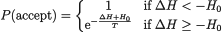
\includegraphics[width=0.7\textwidth,height=\textheight]{images/acceptance.png}

}

\caption{Equation 1.}

\end{figure}%

In the above equation, \emph{T} is a parameter that determines how
likely it is that an unfavorable copy attempt that increases the energy
is accepted, while \emph{H0} is a parameter representing the yield, that
is, how easily the cell membrane changes shape (often, this parameter is
set to \emph{H0 = 0}). What this equation says is: Configurational
changes that lower the energy below at least \emph{H0} are always
accepted (probability of 1), while configurational changes that increase
the energy are accepted with a probability that decreases exponentially
with the energy cost. In a biological sense, cells consume energy from
ATP to create configurations that are physically unfavorable (\emph{ΔH ≥
-H0}). Therefore, the parameter \emph{T} can be interpreted as intrinsic
cell activity.

\section{Exercises}\label{exercises}

\begin{exercise}[Algorithmic thinking - Anatomy of a cellular Potts
model]\protect\hypertarget{exr-non}{}\label{exr-non}

A minimal cellular Potts model simulation of cell sorting contains the
following ingredients:

\begin{itemize}
\tightlist
\item
  definition of the ``sigma field''
\item
  definition of the ``tau field''
\item
  the initial condition of sigma and tau fields
\item
  the neighborhood of a grid site
\item
  a Monte Carlo stepping procedure
\item
  definition and calculation of the energy function H
\end{itemize}

Study the code provided in the script \texttt{01\_cpm.py}. Then, answer
the following questions:

\begin{itemize}
\tightlist
\item
  Which functions in the script correspond to the above ingredients?
\item
  What is the default initial condition?
\item
  What is the default neighborhood?
\item
  Run the script and observe the plots that appear. Explain in your own
  words what is the sigma field and what is the tau field. Do you
  understand why two different fields are needed?
\end{itemize}

\end{exercise}

\begin{exercise}[Conceptual thinking - Interpreting the Hamiltonian
energy function]\protect\hypertarget{exr-non}{}\label{exr-non}

The \textbf{Hamiltonian} energy function \emph{H} is at the heart of a
CPM/GGH simulation. \emph{H} reflects our assumptions about the system
and how forces affect the cell (the derivative of energy with respect to
position is force).

In the script \texttt{01\_cpm.py}, the following Hamiltonian is used.

\begin{figure}[H]

{\centering 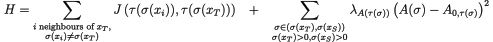
\includegraphics{images/Hamiltonian.png}

}

\caption{Equation 2.}

\end{figure}%

where \emph{J} is a symmetric matrix of interfacial energies for all
cell type pairs \emph{τ} (small Greek letter tau), \emph{A(σ)} is the
area sum of lattice sites belonging to spin \emph{σ}, \emph{A0,τ(σ)} is
the ``target'' area of the corresponding cell type \emph{τ}, and
\emph{λA(τ(σ))} is a weighting factor that scales the importance of this
term (also known as \textbf{Lagrange multiplier}). Each term represents
a \textbf{constraint}.

Perhaps a more intuitive way to understand the terms is the following
pseudo-code:

\includegraphics[width=1.3\textwidth,height=\textheight]{images/pseudocode_table.png}

Compare the pseudo-code to the implementation in the script. Then answer
the following questions:

\begin{itemize}
\tightlist
\item
  What are the biological processes modeled with this specific energy
  function?
\item
  Take a closer look at the summation terms. Over which domain is the
  first sum calculated? What about the second summation term?
\end{itemize}

\end{exercise}

\begin{exercise}[Conceptual thinking - How parameters affect the
Hamiltonian energy
function]\protect\hypertarget{exr-non}{}\label{exr-non}

The modified Metropolis algorithm used in the Monte Carlo stepping
procedure ensures that over time, on average, the sum of the energy of
the entire sigma field will reach a minimum. However, the different
Hamiltonian terms may work ``against'' each other: minimizing one term
may lead to maximizing the value of the other term.

Let's vary the parameters that affect the Hamiltonian terms to get an
intuition for how they work. In the following, you may want to take
screenshots of the final simulation state to put in your notes, so that
it's easier to compare the outputs.

\begin{itemize}
\tightlist
\item
  Change the default neighborhood to \texttt{“8”} and run the simulation
  again. What happens?
\item
  Keep the neighborhood at \texttt{“8”}, and increase the parameter for
  \texttt{“volume\_weight”} from \texttt{{[}1,\ 1{]}} to
  \texttt{{[}2,\ 1{]}}. Then, run the simulation again. What happens?
\item
  Change the initialization mode (\texttt{“init\_mode”}) from
  \texttt{“random\_pixel”} to \texttt{“square\_grid”}, and reset the
  parameter \texttt{“volume\_weight”} to \texttt{{[}1,\ 1{]}}. What
  happens now if you simulate?
\item
  Explain why these settings and parameters that you just changed affect
  the simulation outcome.
\end{itemize}

\end{exercise}

\begin{exercise}[Algorithmic thinking - The Monte Carlo update
algorithm]\protect\hypertarget{exr-non}{}\label{exr-non}

In addition to showing a visualization of the \emph{σ} and \emph{τ}
fields, the script \texttt{01\_cpm.py} also prints some information to
the terminal.

Reset all parameters to their default values, then, based on the printed
information, answer the following questions:

\begin{itemize}
\tightlist
\item
  How many copy attempts are made in total in one Monte Carlo Step?
\item
  How many of these copy attempts are accepted on average?

  \begin{itemize}
  \tightlist
  \item
    Calculate the average for 5 Monte Carlo Steps across 3 simulation
    runs.
  \end{itemize}
\item
  How many seconds does it take to run one simulation?

  \begin{itemize}
  \tightlist
  \item
    Calculate the average run time for 3 runs.
  \end{itemize}
\end{itemize}

The script \texttt{01\_cpm.py} uses the traditional update algorithm. In
this algorithm, every copy attempt picks a target site randomly among
all lattice sites, then subsequently picks a source site randomly among
the neighbors of the target site. This leads to many invalid lattice
pairs that are always rejected. The edge list algorithm is a clever way
of speeding up this procedure by restricting copy attempts only to those
interfaces where there is a possibility of acceptance.

\begin{figure}[H]

{\centering \includegraphics{images/edgelist.png}

}

\caption{Since a copy attempt affects a pair of neighboring lattice
sites, we can keep track of valid pairs (productive site pairs). These
can be represented by an edge, i.e.~an arrow pointing from one site to
the other. Edges have a directionality, so two neighboring sites are
always joined by two edges with opposing direction.}

\end{figure}%

The script \texttt{02\_cpm\_edgelist.py} implements the edge list
algorithm. It's quite complicated, so don't worry about understanding
all the technical details. Using this script, answer the above questions
again and compare to the results you got with the traditional update
algorithm.

Explain: Why does the edgelist algorithm reduce computation time? In
which situations would you expect the difference in computation time
between algorithms to be large?

\end{exercise}

\begin{exercise}[Biology - Expanding the
Hamiltonian]\protect\hypertarget{exr-non}{}\label{exr-non}

Suppose you want to add more mechanisms for cell shape changes to the
model. This would involve the following steps:

\begin{enumerate}
\def\labelenumi{\arabic{enumi}.}
\tightlist
\item
  Coming up with a hypothesis on how forces act on the cell shape.
\item
  Deriving a mathematical function that establishes the energy balance.
\item
  Add an additional function to the code that calculates the energy
  based on the cell configuration.
\item
  Call this function in the code that calculates the energy
  differential.
\end{enumerate}

Let's walk through these steps together to create a \textbf{perimeter
constraint}.

\begin{enumerate}
\def\labelenumi{\arabic{enumi}.}
\item
  Animal cells possess a contractile actomyosin cortex connected to the
  cell membrane via actin-membrane linker proteins. Cortex contraction
  is regulated to maintain homeostasis of the membrane tension. Simply
  put, if the cell membrane gets ``floppy'', the cortex contracts to
  pull the membrane in. Vice-versa, if the membrane is too tense, cortex
  contractility is reduced to allow the membrane to relax. We thus could
  advance the hypothesis that forces from the actin cortex strive to
  maintain a constant cell surface area.
\item
  We want cell surface area to reach a target homeostatic value
  \emph{S0}. Let's call the actual cell surface area \emph{S}. We need a
  function that has a minimum where \emph{S0 = S} and increases if
  \emph{S} is larger or smaller than \emph{S0}. A simple function that
  does the trick is the parabola \emph{(S- S0)2}. We may also want to
  tune how much this term influences the entire Hamiltonian, so we
  introduce the weight factor \emph{λS}. We also consider that both
  \emph{S0} and \emph{λS} may depend on cell type \emph{τ}.
\end{enumerate}

Thus, we write:

\begin{figure}

{\centering 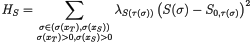
\includegraphics[width=0.6\textwidth,height=\textheight]{images/perimeter.png}

}

\caption{Equation 3.}

\end{figure}%

\begin{itemize}
\tightlist
\item
  For the implementation of steps 3 and 4, consult the script
  \texttt{03\_cpm\_perimeter.py}.
\item
  Study the new additions to the script (search for the string:
  \texttt{\#\#\#\ NEW\ \#\#\#} to find them quickly), then run the
  simulation. Vary the parameters to gain an intuition of how this new
  Hamiltonian term affects the simulation outcome.
\item
  You may have noticed the simulation is running more slowly than
  before. Review the new code additions again. Can you identify any
  potential reasons for this decrease in computation speed?
\end{itemize}

\end{exercise}

\begin{exercise}[Biology - Imposing cell
connectivity]\protect\hypertarget{exr-non}{}\label{exr-non}

In the previous simulations you ran, you may have noticed that cells
sometimes break up into disjointed fragments. There are two alternative
ways to prevent this: 1. Add a new Hamiltonian term that penalizes copy
attempts that would break up the cell. 2. Modify the update algorithm to
always reject copies that would break cells apart.

Script \texttt{04\_cpm\_connectivity.py} implements the second option
using a flood fill algorithm to count the number of contiguous pixels of
the non-medium target cell supposing that a copy succeeded.

Try out the simulation!

\begin{itemize}
\tightlist
\item
  Can you think of advantages and disadvantages to using the first or
  second option?
\item
  Once again, the simulation is running more slowly than before. What
  parts of the new code do you suspect may be causing the slowdown?
\end{itemize}

\end{exercise}

\begin{exercise}[Biology - Exploring differential adhesion and cell
sorting]\protect\hypertarget{exr-non}{}\label{exr-non}

Now let's explore how changing adhesion affinities leads to different
sorted cell configurations. To do that, you will need to run simulations
for a longer time. To speed up computations, you will be using an
optimized package (many scripts working together), which is contained in
the folder \texttt{“cellularPotts”}. To make visualizations super-fast,
this package uses the \texttt{PyQt5} module, which should be installed
by default with your Anaconda distribution.

\emph{Note: If for some reason you cannot get \texttt{PyQt5} to work,
there is an alternative package that uses matplotlib
\texttt{“cellularPotts\_MPL”}. However, this runs much slower.}

To launch the simulation, run the \texttt{main.py} file in the
\texttt{cellularPotts} folder. You can change the parameters by
adjusting values in the \texttt{parameters.py} file.

Adjust the values of the adhesion table for the two cell types:

\begin{itemize}
\tightlist
\item
  Set equal adhesion affinities for all cell-cell interactions. Leave
  affinity to the medium at a low value.
\item
  Set the adhesion affinity of cell type 1 to itself to a larger value.
\item
  Set the affinities such that cell-medium interactions are more
  favorable than any cell-cell interactions.
\item
  Explore how other parameters such as volume and surface constraints
  affect the cell sorting simulations.
\end{itemize}

\emph{(Master students)} Add a third cell type to the simulation by
editing the \texttt{parameter.py} file. Can you get a sorted
configuration where cell type 1 envelops cell type 2, which itself
envelops cell type 3?

\end{exercise}

\subsubsection{References}\label{references-1}

{[}1{]} Gilbert and Barresi (2016)
(https://utrechtuniversity.on.worldcat.org/oclc/1035852599)

{[}2{]} Graner and Glazier (1992)
(https://doi.org/10.1103/PhysRevLett.69.2013)

\part{III) Cell differentiation}

\chapter{Cell differentiation
introduction}\label{cell-differentiation-introduction}

\begin{figure}

{\centering \includegraphics[width=1.5\textwidth,height=\textheight]{images/0-ecoli-regulondb_doi.png}

}

\caption{Gene regulation in a bacteria: from genes to networks. Credit:
RegulonDB, and DOI: 10.1371/journal.pone.0106479}

\end{figure}%

Cell differentiation is the process in which cells acquire specialized
functions, giving rise to a large array of different cell types. This
happens in single cell organisms (bacterial cells being in exponential
growth or stationary phase), and multicellular organisms (with different
cell types organized in tissues and organs). This cell specialization
results from regulated gene expression: genes are turned on and off in
precise combinations, yielding distinct expression profiles. Therefore,
cells with an identical genome can be phenotypically different if they
express different sets of genes. Yet, how exactly is this differential
gene expression regulated?

Transcription factors are DNA-binding proteins that regulate gene
transcription by binding to gene promoters to switch gene expression
\(ON\) or \(OFF\), therefore acting as master regulators of gene
expression. In \emph{E. coli}, plants and animals it is estimated that
5-10\% of the genes are transcription factors, and then this relative
small portion of the genome controls the expression of the rest of the
genes. Numerous transcription factors together with signaling pathways
(\ldots{} and epigenetic modifications) form gene regulatory networks
that govern when and where genes are expressed. Computational models are
useful to study how transcription factor activity is regulated, and
describe the mechanisms underlying cell identity and behavior. For
example, they can help us decipher how gene regulatory networks produce
the gene expression patterns observed in \emph{normal} and
\emph{abnormal} development (where cells do not differentiate normally),
or identify information processing motifs in the network that help cells
make decisions in response to intrinsic cues and environmental signals.

In this part of the course, you will learn how to use computational
models to simulate gene regulatory networks and to understand how their
dynamics generate gene expression patterns that establish and maintain
different cell types.

\chapter{Gene regulation in time}\label{gene-regulation-in-time}

\section{Introduction}\label{introduction}

In this practical you will get hands on experience into making gene
regulatory networks models. First you will practice how to encode
regulatory interactions into ordinary differential equations and logical
rules. Next you will study how many interactions produce self-sustained
activity configurations (attractors) in a Boolean network model (Rozum
et al. (2023)). Lastly, you will learn how to predict the genes that
cause cell fate transitions (attractor changes).

Today we will use the following python file:
\texttt{circuitsfunctions.py}. In it you will find the code of the
functions we use throughout the practical, have a quick look at it.

\section{Regulatory interactions}\label{regulatory-interactions}

Open Boolean\_practical.py and familiarize yourself with the functions
\texttt{ODEgeneRegulation()} and \texttt{logicalRule()}. Look at the
name of the functions, inputs and outputs.

Both functions model an \texttt{AND} gate where nodeA and nodeB
positively regulate nodeC. This could represent that A and B are
transcription factors that form a protein complex, and that it is via
this complex that they can regulate the expression of C.

While \texttt{ODEgeneRegulation()} encodes this regulation with an
ordinary differential equation that requires several parameters,
\texttt{logicalRule()} only needs the logical operator relating the
input genes.

\textbf{ODE implementation}

\(\frac{dC}{dt}=p\frac{A^n}{K^n+A^n}\frac{B^n}{K^n+B^n}-dC\)

Where \(p\) is the production rate, \(K\) is the half saturation
constant (represents the affinity of a TF to the promoter), \(n\) is the
cooperativity of transcription factor binding, and is the same for \(A\)
and \(B\), \(d\) is the decay rate.

\textbf{Logical rule implementation}

\(C_{t+1}=A_t\) \& \(B_t\)

\textbf{Python code for ODE and logical rule}

\begin{Shaded}
\begin{Highlighting}[]
\KeywordTok{def}\NormalTok{ ODEgeneRegulation(a,t,parameters): }
\NormalTok{    prod}\OperatorTok{=}\NormalTok{parameters[}\StringTok{\textquotesingle{}prod\textquotesingle{}}\NormalTok{]}
\NormalTok{    decay}\OperatorTok{=}\NormalTok{parameters[}\StringTok{\textquotesingle{}decay\textquotesingle{}}\NormalTok{]}
\NormalTok{    Ksat}\OperatorTok{=}\NormalTok{parameters[}\StringTok{\textquotesingle{}Ksat\textquotesingle{}}\NormalTok{]}
\NormalTok{    nodeA}\OperatorTok{=}\NormalTok{parameters[}\StringTok{\textquotesingle{}nodeA\textquotesingle{}}\NormalTok{]}
\NormalTok{    nodeB}\OperatorTok{=}\NormalTok{parameters[}\StringTok{\textquotesingle{}nodeB\textquotesingle{}}\NormalTok{]}
\NormalTok{    n}\OperatorTok{=}\NormalTok{parameters[}\StringTok{\textquotesingle{}n\textquotesingle{}}\NormalTok{]}
\NormalTok{    outputC}\OperatorTok{=}\NormalTok{a[}\DecValTok{0}\NormalTok{]}
\NormalTok{    doutputC}\OperatorTok{=}\NormalTok{prod}\OperatorTok{*}\NormalTok{nodeA}\OperatorTok{**}\NormalTok{n}\OperatorTok{/}\NormalTok{(Ksat}\OperatorTok{**}\NormalTok{n}\OperatorTok{+}\NormalTok{nodeA}\OperatorTok{**}\NormalTok{n)}\OperatorTok{*}\NormalTok{nodeB}\OperatorTok{**}\NormalTok{n}\OperatorTok{/}\NormalTok{(Ksat}\OperatorTok{**}\NormalTok{n}\OperatorTok{+}\NormalTok{nodeB}\OperatorTok{**}\NormalTok{n)}\OperatorTok{{-}}\NormalTok{decay}\OperatorTok{*}\NormalTok{outputC }\CommentTok{\#Tip: Change this in exercise 8.3}
    \ControlFlowTok{return}\NormalTok{(doutputC)}

\KeywordTok{def}\NormalTok{ logicalRule(nodeA,nodeB):}
    \ControlFlowTok{return}\NormalTok{(nodeA }\KeywordTok{and}\NormalTok{ nodeB)}
\end{Highlighting}
\end{Shaded}

\begin{exercise}[Mathematical
thinking]\protect\hypertarget{exr-non}{}\label{exr-non}

What is the minimum information you need to encode a regulatory
interaction with either function? In what cases would you prefer to use
an ODE or a logical rule for a model?

\end{exercise}

Let's run the model to simulate what happens if \texttt{A} and
\texttt{B} are both active/expressed. Do this using the
\texttt{ODEgeneRegulation()} and \texttt{logicalRule()} functions.
Create a new python file, import \texttt{circuitfunctions.py} and copy
the following lines of code inside the main().

\begin{Shaded}
\begin{Highlighting}[]
\CommentTok{\# ODErun has three arguments: model, geneA, geneB}
\NormalTok{A}\OperatorTok{=}\DecValTok{10}
\NormalTok{B}\OperatorTok{=}\DecValTok{10}
\NormalTok{ODErun(ODEgeneRegulation,A,B) }

\CommentTok{\# Boolean model}
\CommentTok{\# look at the text in the terminal for the result:}
\NormalTok{A}\OperatorTok{=}\DecValTok{1}
\NormalTok{B}\OperatorTok{=}\DecValTok{1}
\BuiltInTok{print}\NormalTok{(}\StringTok{"the boolean operation of nodeA "}\NormalTok{,A,}\StringTok{" AND nodeB"}\NormalTok{,B,}\StringTok{" is:"}\NormalTok{, logicalRule(A,B))}
\end{Highlighting}
\end{Shaded}

Both implementations of this regulatory interaction produce the same
effect, i.e.~\texttt{C} is active when both \texttt{A} and \texttt{B}
are active. Yet, the ODE version recovers quantitative differences in
\texttt{C} activity with values higher than 1.

Now, let's explore the output of each function using different values of
\texttt{A} and \texttt{B} We are going to use the code below to plot the
output of the ODE and the Boolean model in a 2D heatmap. Notice that the
exploration values for the ODE model is 11 values
(0,1,2,3,4,5,6,7,8,9,10), while for a Boolean model is 2 (0 or 1).

ODE model simulation - AND gate:

\begin{Shaded}
\begin{Highlighting}[]
\NormalTok{explorationvalue }\OperatorTok{=} \DecValTok{11} \CommentTok{\# an ODE model allows us to explore more values than a Boolean model}
\NormalTok{ode\_output }\OperatorTok{=}\NormalTok{ np.zeros((explorationvalue, explorationvalue))}
\ControlFlowTok{for}\NormalTok{ nodeA }\KeywordTok{in} \BuiltInTok{range}\NormalTok{(}\DecValTok{0}\NormalTok{, explorationvalue):}
    \ControlFlowTok{for}\NormalTok{ nodeB }\KeywordTok{in} \BuiltInTok{range}\NormalTok{(}\DecValTok{0}\NormalTok{, explorationvalue):}
\NormalTok{        parameters }\OperatorTok{=}\NormalTok{ \{}\StringTok{\textquotesingle{}prod\textquotesingle{}}\NormalTok{: }\FloatTok{0.01}\NormalTok{, }\StringTok{\textquotesingle{}decay\textquotesingle{}}\NormalTok{: }\FloatTok{0.001}\NormalTok{,}\StringTok{\textquotesingle{}Ksat\textquotesingle{}}\NormalTok{: }\DecValTok{4}\NormalTok{, }\StringTok{\textquotesingle{}n\textquotesingle{}}\NormalTok{: }\DecValTok{2}\NormalTok{,}\StringTok{\textquotesingle{}nodeA\textquotesingle{}}\NormalTok{:nodeA,}\StringTok{\textquotesingle{}nodeB\textquotesingle{}}\NormalTok{:nodeB\} }\CommentTok{\# prod, decay, Ksat, n, and initial values for A and B}
\NormalTok{        cells }\OperatorTok{=}\NormalTok{ odeint(ODEgeneRegulation, }\DecValTok{0}\NormalTok{, np.arange(}\DecValTok{0}\NormalTok{, }\FloatTok{1000.1}\NormalTok{ , }\FloatTok{0.1}\NormalTok{), args}\OperatorTok{=}\NormalTok{(parameters,)) }
\NormalTok{        ode\_output[nodeA, nodeB] }\OperatorTok{=}\NormalTok{ cells[}\OperatorTok{{-}}\DecValTok{1}\NormalTok{, }\DecValTok{0}\NormalTok{]}
\end{Highlighting}
\end{Shaded}

Boolean network simulation - AND gate:

\begin{Shaded}
\begin{Highlighting}[]
\NormalTok{explorationvalue}\OperatorTok{=}\DecValTok{2} \CommentTok{\# a Boolean model assumes there is only 2 possible states: 0 or 1}
\NormalTok{bool\_output }\OperatorTok{=}\NormalTok{ np.zeros((explorationvalue, explorationvalue))}
\ControlFlowTok{for}\NormalTok{ nodeA }\KeywordTok{in} \BuiltInTok{range}\NormalTok{(}\DecValTok{0}\NormalTok{, explorationvalue):}
    \ControlFlowTok{for}\NormalTok{ nodeB }\KeywordTok{in} \BuiltInTok{range}\NormalTok{(}\DecValTok{0}\NormalTok{, explorationvalue):}
\NormalTok{        bool\_output[nodeA, nodeB] }\OperatorTok{=}\NormalTok{ nodeA }\KeywordTok{and}\NormalTok{ nodeB }\CommentTok{\#AND \#Tip: Change this in exercise 8.3}
\end{Highlighting}
\end{Shaded}

After running each, this function plots the ODE and Boolean results side
by side:

\begin{Shaded}
\begin{Highlighting}[]
\NormalTok{ODEBooleanPlot(ode\_output, bool\_output)}
\end{Highlighting}
\end{Shaded}

\begin{exercise}[Biology]\protect\hypertarget{exr-non}{}\label{exr-non}

What similarties and differences in the activity of \(C\) do you see
using each approach? Why is the activity of \(C\) higher in the ODE
output than the Boolean one?

\end{exercise}

\begin{exercise}[Altorithmic
thinking:]\protect\hypertarget{exr-non}{}\label{exr-non}

Now let's compare how ODE and Boolean models represent different
regulatory interactions. You can use the same code in the previous box.
Remember to modify the logical operator in the Boolean section, and to
modify the \(doutputC\) equation in the \texttt{ODEgeneRegulation}
function:

\begin{enumerate}
\def\labelenumi{\arabic{enumi}.}
\tightlist
\item
  Either \texttt{A} or \texttt{B} can activate \texttt{C}.
\item
  \texttt{A} represses \texttt{C}.
\item
  \texttt{A} and \texttt{B} together repress \texttt{C}.
\item
  \texttt{A} represses \texttt{C} and \texttt{B} activates it.
\item
  \texttt{A} or \texttt{B} can activate \texttt{C}, but not when both
  are active at the same time.
\item
  any other biological scenario yon can think of!
\end{enumerate}

\begin{itemize}
\tightlist
\item
  See if you can modify the code to include an extra input node, and
  make a 3-node logical gate.
\end{itemize}

\end{exercise}

\begin{exercise}[Biology and Algorithmic
thinking]\protect\hypertarget{exr-non}{}\label{exr-non}

Is there a logical gate that can be better represented with an ODE than
with Boolean logic? Give an\\
examples of biological regulatory interactions that can be described
with each logical gate?

\end{exercise}

\section{Gene regulatory network}\label{gene-regulatory-network}

Now let's move to a network model made of many individual regulatory
interactions (Garcı́a-Gómez et al. (2020)). This model includes
regulatory interactions discovered for the cells of plant roots in years
of experimental research. Here, all this knowledge is encoded as logical
rules.

The model consists of 18 variables representing transcription factors,
hormones, peptides. Look at the \texttt{rootNetwork()} function in the
\texttt{circuitFunctions.py} file. This function defines the state of 18
variables (CK, ARR1, SHY2, AUXIAAR, etc.) based on an input stored in
\texttt{parameters}, then it updates the state of each variable using
the logical operators \(AND\), \(OR\) and \(NOT\); the result is stored
in \texttt{w\_variable}. The function returns the update state
\texttt{w\_variable} for each of the 18 variables.

\subsection{Initial condition
timecourse}\label{initial-condition-timecourse}

Let us define a random initial condition for each of these 18 variables
, and the total number of timesteps we will solve the network using the
logical functions. First, we need to input the initial condition of the
variables to \texttt{rootNetwork()} using \texttt{parameters}. Next, we
save the output of this function as the new current state. We repeat
this procedure iteratively for as many timesteps as we defined, saving
in a matrix the timecourse of the simulation. This can be done using a
for loop as shown below:

\begin{Shaded}
\begin{Highlighting}[]
\NormalTok{timesteps}\OperatorTok{=}\DecValTok{20}
\NormalTok{variables}\OperatorTok{=}\DecValTok{18}
\NormalTok{matrix }\OperatorTok{=}\NormalTok{ np.zeros((timesteps}\OperatorTok{+}\DecValTok{1}\NormalTok{, variables), dtype}\OperatorTok{=}\BuiltInTok{int}\NormalTok{) }
\NormalTok{matrix[}\DecValTok{0}\NormalTok{,:] }\OperatorTok{=}\NormalTok{ np.random.randint(}\DecValTok{0}\NormalTok{, }\DecValTok{2}\NormalTok{, size}\OperatorTok{=}\NormalTok{variables) }\CommentTok{\#Random initial condition}
\ControlFlowTok{for}\NormalTok{ i }\KeywordTok{in} \BuiltInTok{range}\NormalTok{(timesteps):}
\NormalTok{    parameters}\OperatorTok{=}\NormalTok{ \{}\StringTok{\textquotesingle{}CK\textquotesingle{}}\NormalTok{: matrix[i,}\DecValTok{0}\NormalTok{], }\StringTok{\textquotesingle{}ARR1\textquotesingle{}}\NormalTok{: matrix[i,}\DecValTok{1}\NormalTok{], }\StringTok{\textquotesingle{}SHY2\textquotesingle{}}\NormalTok{: matrix[i,}\DecValTok{2}\NormalTok{], }\StringTok{\textquotesingle{}AUXIAAR\textquotesingle{}}\NormalTok{: matrix[i,}\DecValTok{3}\NormalTok{], }\StringTok{\textquotesingle{}ARFR\textquotesingle{}}\NormalTok{: matrix[i,}\DecValTok{4}\NormalTok{], }\StringTok{\textquotesingle{}ARF10\textquotesingle{}}\NormalTok{: matrix[i,}\DecValTok{5}\NormalTok{], }\StringTok{\textquotesingle{}ARF5\textquotesingle{}}\NormalTok{: matrix[i,}\DecValTok{6}\NormalTok{], }\StringTok{\textquotesingle{}XAL1\textquotesingle{}}\NormalTok{: matrix[i,}\DecValTok{7}\NormalTok{], }\StringTok{\textquotesingle{}PLT\textquotesingle{}}\NormalTok{: matrix[i,}\DecValTok{8}\NormalTok{], }\StringTok{\textquotesingle{}AUX\textquotesingle{}}\NormalTok{: matrix[i,}\DecValTok{9}\NormalTok{], }\StringTok{\textquotesingle{}SCR\textquotesingle{}}\NormalTok{: matrix[i,}\DecValTok{10}\NormalTok{], }\StringTok{\textquotesingle{}SHR\textquotesingle{}}\NormalTok{: matrix[i,}\DecValTok{11}\NormalTok{], }\StringTok{\textquotesingle{}MIR165\textquotesingle{}}\NormalTok{: matrix[i,}\DecValTok{12}\NormalTok{], }\StringTok{\textquotesingle{}PHB\textquotesingle{}}\NormalTok{: matrix[i,}\DecValTok{13}\NormalTok{], }\StringTok{\textquotesingle{}JKD\textquotesingle{}}\NormalTok{: matrix[i,}\DecValTok{14}\NormalTok{], }\StringTok{\textquotesingle{}MGP\textquotesingle{}}\NormalTok{: matrix[i,}\DecValTok{15}\NormalTok{], }\StringTok{\textquotesingle{}WOX5\textquotesingle{}}\NormalTok{: matrix[i,}\DecValTok{16}\NormalTok{], }\StringTok{\textquotesingle{}CLE40\textquotesingle{}}\NormalTok{: matrix[i,}\DecValTok{17}\NormalTok{]\}}
    
\NormalTok{    matrix[i}\OperatorTok{+}\DecValTok{1}\NormalTok{, :] }\OperatorTok{=}\NormalTok{ rootNetwork(parameters) }\CommentTok{\# we save the output in i+1}

\NormalTok{plotBooleanTimecourse(matrix,timesteps)}
\end{Highlighting}
\end{Shaded}

At the end the function \texttt{plotBooleanTimecourse()} will make a
plot to see how each variable in the network changes ts activity
throughout the simulated timesteps. 100 timesteps is enough to reach an
attractor for this network.

\begin{itemize}
\tightlist
\item
  For the initial condition you can also use that of one of the
  attractors reported in the paper and check what happens when you
  update them.
\end{itemize}

\begin{exercise}[Algorithmic
thinking]\protect\hypertarget{exr-non}{}\label{exr-non}

Try this initial condition:

\begin{Shaded}
\begin{Highlighting}[]
\NormalTok{matrix[}\DecValTok{0}\NormalTok{,:]}\OperatorTok{=}\NormalTok{[}\DecValTok{0}\NormalTok{,}\DecValTok{1}\NormalTok{,}\DecValTok{1}\NormalTok{,}\DecValTok{0}\NormalTok{,}\DecValTok{1}\NormalTok{,}\DecValTok{1}\NormalTok{,}\DecValTok{0}\NormalTok{,}\DecValTok{0}\NormalTok{,}\DecValTok{1}\NormalTok{,}\DecValTok{0}\NormalTok{,}\DecValTok{1}\NormalTok{,}\DecValTok{1}\NormalTok{,}\DecValTok{1}\NormalTok{,}\DecValTok{1}\NormalTok{,}\DecValTok{1}\NormalTok{,}\DecValTok{0}\NormalTok{,}\DecValTok{1}\NormalTok{,}\DecValTok{0}\NormalTok{]}
\end{Highlighting}
\end{Shaded}

Solve this initial condition using \texttt{rootNetwork()} and
\texttt{rootNetworkAsynchronous()}. Compare the output in each case.
What happens and why? What does an asynchronous update do?

\end{exercise}

This network has 18 variables, and then \(2^{18}\) = 262,144 possible
states. We can solve each of these conditions, or instead explore just a
subset of them.

\begin{exercise}[Algorithmic
thinking]\protect\hypertarget{exr-non}{}\label{exr-non}

Using the previous code, add for loop to solve 100 random initial
conditions, and then save the final activity configurations (attractors)
in the attractors matrix. The attractors matrix should have the
dimensions\\
(initial\_conditions, variables) so that you can plot the results using
the \texttt{plotBooleanAttractors()} function.

\begin{itemize}
\item
  Notice here you should save the final state for each initial condition
  you explore.
\item
  tip: 100 initial conditions is a good number to explore.
\end{itemize}

\begin{Shaded}
\begin{Highlighting}[]
\NormalTok{ICs}\OperatorTok{=}\DecValTok{100}
\NormalTok{attractors }\OperatorTok{=}\NormalTok{ np.zeros((ICs, }\BuiltInTok{len}\NormalTok{(parameters))) }

\CommentTok{\# your code}

\NormalTok{plotBooleanAttractors(attractors) }\CommentTok{\# it takes as argument a matrix of attractors}
\end{Highlighting}
\end{Shaded}

\end{exercise}

You probably found many different attractors. First, let's use a
multidimensional reduction technique to see how these attractors relate
to each other.

\begin{Shaded}
\begin{Highlighting}[]
\NormalTok{UMAPBoolean(attractors)}
\end{Highlighting}
\end{Shaded}

\begin{exercise}[Biology / Conceptual
thinking]\protect\hypertarget{exr-non}{}\label{exr-non}

\textbf{Q5} Why do you see clearly defined groups and not a continuous
distribution of attractors?

\end{exercise}

Now let's analyse the attractors you found. First, let's group similar
attractors using the \texttt{sorted()} function:

\begin{Shaded}
\begin{Highlighting}[]
\NormalTok{attractors\_sorted }\OperatorTok{=}\NormalTok{ np.array(}\BuiltInTok{sorted}\NormalTok{(attractors.tolist()))}
\NormalTok{plotBooleanAttractors(attractors\_sorted) }
\end{Highlighting}
\end{Shaded}

\begin{exercise}[Biology / Conceptual
thinking]\protect\hypertarget{exr-non}{}\label{exr-non}

\textbf{Q6} Do some attractors occur more frequently than others. Why is
this?

\end{exercise}

\begin{exercise}[Biology]\protect\hypertarget{exr-non}{}\label{exr-non}

Some variables are active (1) in the majority of the attractors, others
in half, and others in very few. In how many attractors is the node SHR
active? What does this suggest about its regulation?

\end{exercise}

Now let's remove the repeated rows (duplicate attractor states) to see
unique attractors using the \texttt{np.unique()} function:

\begin{Shaded}
\begin{Highlighting}[]
\NormalTok{\_, unique\_indices }\OperatorTok{=}\NormalTok{ np.unique(attractors, axis}\OperatorTok{=}\DecValTok{0}\NormalTok{, return\_index}\OperatorTok{=}\VariableTok{True}\NormalTok{)}
\NormalTok{attractors\_unique }\OperatorTok{=}\NormalTok{ attractors[np.sort(unique\_indices)]}
\NormalTok{plotBooleanAttractors(attractors\_unique) }
\end{Highlighting}
\end{Shaded}

\begin{exercise}[Biology / conceptual
thinking]\protect\hypertarget{exr-non}{}\label{exr-non}

How many unique attractors did you find? Compare them with the ones
reported in the paper. Are they all fixed points?

\end{exercise}

\section{Cell differentiation -- jumping from one attractor to
another}\label{cell-differentiation-jumping-from-one-attractor-to-another}

Depending on what we want to answer a continuous or discrete model may
be more appropriate for a model. To study the role of many genes in cell
differentiation, a Boolean model might be better particularly if we lack
details of the parameters underlying each reaction. If we want to study
how cells jump from one state to another, a continuous model might be
more appropriate.

Here we will see how we can convert the Boolean model to a continuous
one and use it to predict which regulators are able of causing a change
in the state of the system (changes in cell fate!)

Compare the code of the functions rootNetwork() and rootNetworkODE().
Notice how in rootNetworkODE() the logical rules are represented with
min and max functions, and then used in a sigmoidal function to create a
continuous ODE model. * AND operator is a min function, OR operator is a
max function, and NOT operator is 1-x. Use the code below to run a
random initial condition for the 18 variables (IC) and see how the
system behaves.

\begin{Shaded}
\begin{Highlighting}[]
\NormalTok{timerunning}\OperatorTok{=}\FloatTok{10.1} 
\NormalTok{times }\OperatorTok{=}\NormalTok{ np.arange(}\DecValTok{0}\NormalTok{, timerunning, }\FloatTok{0.1}\NormalTok{)}

\NormalTok{IC }\OperatorTok{=}\NormalTok{ np.random.randint(}\DecValTok{0}\NormalTok{, }\DecValTok{2}\NormalTok{, size}\OperatorTok{=}\DecValTok{18}\NormalTok{).tolist() }\CommentTok{\#random initial condition}
\NormalTok{parameters }\OperatorTok{=}\NormalTok{ \{}\StringTok{\textquotesingle{}decayrate\textquotesingle{}}\NormalTok{: }\DecValTok{1}\NormalTok{, }\StringTok{\textquotesingle{}h\textquotesingle{}}\NormalTok{: }\DecValTok{50}\NormalTok{\} }
\NormalTok{cells }\OperatorTok{=}\NormalTok{ odeint(rootNetworkODE, IC, times, args}\OperatorTok{=}\NormalTok{(parameters,)) }

\NormalTok{plotODEroot(cells,times)}
\end{Highlighting}
\end{Shaded}

\begin{exercise}[Modeling
choices]\protect\hypertarget{exr-non}{}\label{exr-non}

Do the attractors match those recovered with the Boolean network?

\end{exercise}

Now let's use the model to study cell differentiation. Let's start in
the following initial condition (IC vector), and find a change in a node
that produce a jump to another attractor (end). For this you can simply
flip the activity of a gene in the initial condition (from 0
-\textgreater1 or 1-\textgreater0) and see the final attractor matches
the desired end state.

\begin{Shaded}
\begin{Highlighting}[]
\CommentTok{\# We start here: }
\NormalTok{IC}\OperatorTok{=}\NormalTok{[}\DecValTok{0}\NormalTok{,}\DecValTok{0}\NormalTok{,}\DecValTok{0}\NormalTok{,}\DecValTok{0}\NormalTok{,}\DecValTok{1}\NormalTok{,}\DecValTok{0}\NormalTok{,}\DecValTok{1}\NormalTok{,}\DecValTok{1}\NormalTok{,}\DecValTok{1}\NormalTok{,}\DecValTok{1}\NormalTok{,}\DecValTok{1}\NormalTok{,}\DecValTok{1}\NormalTok{,}\DecValTok{1}\NormalTok{,}\DecValTok{0}\NormalTok{,}\DecValTok{1}\NormalTok{,}\DecValTok{0}\NormalTok{,}\DecValTok{1}\NormalTok{,}\DecValTok{0}\NormalTok{]}
\CommentTok{\# We want to end here. }
\NormalTok{end}\OperatorTok{=}\NormalTok{[}\DecValTok{1}\NormalTok{,}\DecValTok{1}\NormalTok{,}\DecValTok{0}\NormalTok{,}\DecValTok{0}\NormalTok{,}\DecValTok{1}\NormalTok{,}\DecValTok{1}\NormalTok{,}\DecValTok{1}\NormalTok{,}\DecValTok{1}\NormalTok{,}\DecValTok{1}\NormalTok{,}\DecValTok{1}\NormalTok{,}\DecValTok{0}\NormalTok{,}\DecValTok{0}\NormalTok{,}\DecValTok{1}\NormalTok{,}\DecValTok{0}\NormalTok{,}\DecValTok{0}\NormalTok{,}\DecValTok{0}\NormalTok{,}\DecValTok{0}\NormalTok{,}\DecValTok{1}\NormalTok{]}
\CommentTok{\# node order}
\CommentTok{\# CK, ARR1, SHY2, AUXIAAR, ARFR, ARF10, ARF5, XAL1, PLT, AUX, SCR, SHR, MIR165, PHB, JKD, MGP, WOX5, CLE40}

\CommentTok{\# your code }

\NormalTok{plotODErootTransition(cells,times) }\CommentTok{\# use this function to plot your result}
\end{Highlighting}
\end{Shaded}

\begin{exercise}[Algorithmic thinking /
biology]\protect\hypertarget{exr-non}{}\label{exr-non}

What regulator causes the transition between these attractors? How many
variables change their activity between the initial and final state?
what could be the biological meaning of this switch? how would you test
this experimentally?

\end{exercise}

\begin{exercise}[Biology]\protect\hypertarget{exr-non}{}\label{exr-non}

Finally, use the model to predict the rest of the attractor transitions
because of single node changes. Are all attractor transitions possible,
or are there preferred differentiation routes?

\end{exercise}

\section{References}\label{references-2}

\begin{itemize}
\tightlist
\item
  Rozum et al. (2023)
\item
  Garcı́a-Gómez et al. (2020)
\end{itemize}

\chapter{Gene regulation in space}\label{gene-regulation-in-space}

\section*{}\label{section-2}
\addcontentsline{toc}{section}{}

\markright{}

{ \emph{How wonderful that we have met with a paradox. Now we have some
hope of making progress -- Niehls Bohr} }

\section{Auxin does everything}\label{auxin-does-everything}

In this practical you will study the effects of auxin, a plant hormone,
on gene regulation in the root. Auxin is a hormone that is virtually
involved in all developmental processes in plants, from how the plant
embryo is patterned, how the organs in flowers are determined, the
spatial disposition of leaves, among many many others. In each context,
auxin triggers specific responses, posing the question of how is it that
the same molecule can trigger so many different responses. This
specificity of auxin responses can be explained by the underlying
regulatory networks. The auxin signalling pathway activates the auxin
response factors, ARFs, which are transcription factors that regulate
gene expression in response to auxin. Arabidopsis has 23 genes encoding
for ARFs, some regulate gene expression positively and others
negatively, and they are expressed in different tissues. It is this
diversity in transcription factors activity which in part explains how
auxin can regulate so many different things.

\section{Auxin does opposite things in the
root}\label{auxin-does-opposite-things-in-the-root}

Plant roots grow thanks to the presence of stem cells housed in a niche
at the root tip. A subset of these cells express \emph{WOX5},
maintaining the surrounding cells undifferentiated. WOX5 is regulated by
several factors, and network models help us understand how. Researchers
have found paradoxical results regarding how auxin regulates WOX5: some
experiments show that auxin promotes its expression, while others found
it is repressed (Figure 1). Notably, auxin does this opposite regulation
through different ARFs (Figure 2) posing the possibility that accounting
for how the ARFs themselves are regulated can reconcile the results.
Here we will explore this possibility using an \emph{in silico} root
model.

\begin{figure}

{\centering \includegraphics[width=1.3\textwidth,height=\textheight]{images/0-auxin-paradox.png}

}

\caption{Figure 1. The right panel shows evidence of the positive effect
of auxin on WOX5 expression (white arrows). The left panel shows
evidence of auxin repression of WOX5 in the root tip (white rectangle),
also shown with qPCR measurements of WOX5 mRNA in root-tip cells.}

\end{figure}%

The Boolean network we used last week describes the gene and hormonal
activity configurations of the cells in the root tip (Figure 3 left).
This model recovers an attractor representing the columella, the
\textbf{QC}, the endodermis, and three types of vascular cells.
attractors we studied describe the columella, In this model WOX5 is
regulated positively by ARF5, and negatively by ARF10 and also by CLE40.
Both ARF5 and ARF10 are auxin response factors, activated by auxin.
Moreover, other root transcription factors control ARF5 and ARF10
expression causing them to be expressed in specific cells of the root
(see Figure 3). This regulation is included in the Boolean model we
studied last week. Here you will explore whether this is relevant to
understanding the auxin--WOX5 paradox. For this you will use an \emph{in
silico} root model in which each cell carries a copy of the Boolean
network initialized in a particular attractor, which allows us to test
hypotheses and find an explanation.

\begin{figure}

{\centering \includegraphics[width=1\textwidth,height=\textheight]{images/0-unique_attractors-celltypes.png}

}

\caption{Figure 2 Auxin regulates WOX5 expression through different
auxin response factors. These are expressed in specific cell types of
the root}

\end{figure}%

\subsection{Biology / conceptual
thinking}\label{biology-conceptual-thinking-3}

Notice that the QC is the only attractor with WOX5 activity. This makes
sense given that its logical rule is:

\(WOX5_{t+1} =NOT\) \(ARF10\) \(AND\) \(ARF5\) \(AND\) \(NOT\) \(CLE40\)

Notice how the other attractors have either ARF10 and/or CLE40 activity
(repressors of WOX5), or lack ARF5 activity (activator of WOX5). The QC
attractor is the only one with the following combination: ARF5 active,
ARF10 inactive, CLE40 inactive; therefore allowing for WOX5 activity.

\section{The model}\label{the-model}

Today you will use a multicellular model that simulates the cells of a
root tip (Figure 3, right). The tissue is modeled as a grid, where the
\(x\) position defines the radial direction and the \(y\) the
longitudinal position (0 being the cells at the bottom). The cells are
organized in cell layers (8 layers, so \(x\) is 8), each with a gene
regulatory network initialized in a different attractor. The model
simulates the transport of auxin from cell to cell, where the cell type
(the attractor) defines the direction of polar auxin transport. In
figure 3 (right) you can see the different properties that the cells
have: a cell type, auxin levels, gene expression (in the figure we see
only ARF10, ARF5, MGP and WOX5). These properties are stored in
individual grids: one grid for cell type, another for auxin levels, and
many others for each of the genes in the network.

\begin{figure}

{\centering \includegraphics[width=1.3\textwidth,height=\textheight]{images/0-new-RAM.png}

}

\caption{Figure 3. Ingredients of the in silico root model. 1) gene
regulatory network, 2) multi-cellular tissue layout with polar auxin
transport in the root tip}

\end{figure}%

\subsection{Files}\label{files}

1.- \texttt{Rootfunctions.py} -- File storing the functions used in
\texttt{Root-model-Auxin.py}. For this practical you only need to modify
\texttt{rootNetwork}. Yet, have a look at all of them and try to
understand what they do.

The file contains the following functions:

\begin{itemize}
\item
  \texttt{findNeighbors} - retrieves the x and y coordinate of the
  neighbors of a given cell.
\item
  \texttt{auxinTransport} - executes the passive and the polar auxin
  transport using the levels of auxin in each cell stored in
  \texttt{auxinGrid}. The direction at which a cell transports auxin is
  determined by its cell type.
\item
  \texttt{rootNetwork}- stores the interactions of the root network.
  This file is similar to the one we used in the last practical. A key
  difference is that the auxin levels are an input that can modify gene
  expression
  (\texttt{auxininput=parameters{[}\textquotesingle{}auxininput\textquotesingle{}{]}}).
  You will modify this function in question 9.5.
\item
  \texttt{initialCondition} - Initializes the grids of the model. We
  have many cells in this simulation, and we have a grid per cell
  property: cell type (\texttt{cellgrid}), auxin levels
  (\texttt{auxinGrid}), and a grid per node of the network.
\item
  \texttt{nodeUpdate} - function to take the output of the ODE and
  stored it in the grids.
\item
  \texttt{plotGrids} - plots 6 grids you provide. The labelling assumes
  you give \texttt{cellgrid}, \texttt{auxingrid}, \texttt{arf10grid},
  \texttt{arf5grid}, \texttt{mgpgrid}, \texttt{wox5grid.}
\end{itemize}

2.- \texttt{Root-model-Auxin.py} -- code to simulate the \emph{in
silico} root where we use the functions in a specific order. Before the
\texttt{main()} we define the dimensions of the grid, the parameters,
initialize the grid, and then inside the \texttt{main()} we use a for
loop to run the auxin transport and network update for a defined number
of time steps. In this loop, the output of the network is plotted every
10 steps. Tip: if the simulation runs too slow, decrease this plotting
frequency.

3.- \texttt{auxin\_grid.npy} -- initial auxin levels in each cell with
the auxin gradient. This is used to initialize auxinGrid in
\texttt{Root-model-Auxin.py}.

\section{Questions}\label{questions-2}

\begin{exercise}[Algorithmic
thinking]\protect\hypertarget{exr-non}{}\label{exr-non}

Familiarize yourself with the model. Examine \texttt{Rootfunctions.py}.
What are the algorithmic steps you would take if you want to make a
model of the root where cells transport auxin every timestep, and update
their networks every 10 steps? Keep in mind that the cell type of the
cells define the direction at which they transport auxin to their
neighbors. Make a plain-language description.

Tip: have a look at the code in the \texttt{Root-model-Auxin.py}.

\end{exercise}

\begin{exercise}[Biology]\protect\hypertarget{exr-tur}{}\label{exr-tur}

What happens if you update the network more often than the auxin
transport? How would you implement this modification in the code?

\end{exercise}

\begin{exercise}[Biology \& algorithmic
thinking]\protect\hypertarget{exr-tur}{}\label{exr-tur}

Now let's use the model to simulate the auxin treatments from the
experiments in Figure 1. To simulate an auxin treatment change the value
of \(AuxinTreatment\) in \texttt{Root-model-Auxin.py}. Try values of 10
and 750. This increases auxin levels in all cells by the same amount.

\begin{itemize}
\tightlist
\item
  How does auxin treatment affect gene expression in the root?
\item
  Does the model output correspond to the transcriptional reporter of
  WOX5 shown in Figure 1?
\item
  Do you see activation or repression as reported experimentally? (You
  can visualize different genes by changing the grid provided to
  \texttt{plotGrids()}.)
\end{itemize}

\end{exercise}

\begin{exercise}[Biology \& algorithmic/mathematical
thinking]\protect\hypertarget{exr-tur}{}\label{exr-tur}

The model does not yet reproduce the experiments. Yet, we can use this
model to test hypothesis and aim to recover such behaviours (Figure 1).
Let's implement the following two hypotheses:

\begin{figure}

{\centering \includegraphics[width=0.6\textwidth,height=\textheight]{images/0-auxin-hypothesis.png}

}

\caption{Testing two hypothesis: {Auxin represses MGP expression.}
{Extremely high auxin levels (easy to apply experimentally, but
unrealistic \emph{in vivo}) repress WOX5 expression.}}

\end{figure}%

Modify the equations for MGP and WOX5 in \texttt{rootNetwork}
accordingly.

\begin{itemize}
\item
  For MGP, retain its logical rule but multiply its production term by a
  negative regulatory term of auxin (Km = 45): {
  \(\frac{45}{45+auxininput}\) }
\item
  Similarly, add a negative regulation by auxin to the WOX5 equation (Km
  = 1000).
\end{itemize}

Run control and auxin treatments with (i) updated MGP, (ii) updated
WOX5, and (iii) both updates. Use the plotting functions to plot the
final timepoint. It is also interesting to run the timecourse, by
plotting every 10 steps.

Do you now see the differences reported by experimentalists?

\end{exercise}

\begin{exercise}[Biological
interpretation]\protect\hypertarget{exr-tur}{}\label{exr-tur}

You should observe that WOX5 expression gradually expands into the
endodermis and disappears from QC cells when both equations are updated.
This matches the experimental microscopy from Figure 1.

\begin{itemize}
\tightlist
\item
  Why do different parts of the root respond differently to auxin?
\item
  Why does auxin regulation of MGP do? (Tip: look at the network\ldots)
\item
  Why does induction of WOX5 occur mainly in ``upper'' cells and
  repression in the cells closer to the tip?
\end{itemize}

\end{exercise}

\begin{exercise}[Algorithmic
thinking]\protect\hypertarget{exr-tur}{}\label{exr-tur}

Experimental repression of WOX5 was detected by RT-PCR at the very tip
(Figure 1, right panel). Reproduce this \emph{in silico} by saving the
average WOX5 levels of cells at the tip (\texttt{y} \textless{} 40) at
the end of the simulation for all three treatments. For comparison, also
calculate the average for the whole root. Then plot this average WOX5
expression levels (y axis) for each \texttt{auxinTreatment}= 0, 10 and
750 (x axis).

Tip: \texttt{WOX5Grid} stores WOX5 levels, and \(y\) controls the
position of the cells.

What is the overall effect of auxin treatments in the root tip?
Considering that the root contains mixed cell types, which cells best
represent the plotted values?

\end{exercise}

\begin{exercise}[Biology \& algorithmic
thinking]\protect\hypertarget{exr-tur}{}\label{exr-tur}

Now, let's compare WOX5 regulation across tissues. Let's use the model
to do an in RT-PCR \emph{in silico} analysis of only the cells in the QC
position, and also the endodermis cells. This has not been done
experimentally and thus you will generate a prediction (!). Tip: cell
types are stored in \texttt{cellGrid.}

Compare what you see in the root simulation, and what you obtain in the
simulated RT-PCR plot. Which case represents better how WOX5 is
regulated in the root tip? Why?

\end{exercise}

\begin{exercise}[Biology \& algorithmic
thinking]\protect\hypertarget{exr-tur}{}\label{exr-tur}

Changes in WOX5 expression depend on tissue context and auxin dosage.
Simulate a range of auxin treatments from 0 to 750.

Can you now explain the auxin--WOX5 paradox? What mechanism do you
propose?

\end{exercise}

\begin{exercise}[Biology \& conceptual
thinking]\protect\hypertarget{exr-tur}{}\label{exr-tur}

Perform an \emph{in silico} intervention to alter WOX5 dosage
responsiveness to auxin. For example, what would it take to enforce its
continuous expression, or block completely its induction in the
endodermis. How would you test these model predictions experimentally?

\end{exercise}

\begin{exercise}[Biological
thinking]\protect\hypertarget{exr-tur}{}\label{exr-tur}

All models are wrong, but some are useful. The model we studied today
offered us a mechanistic insight into the paradoxical auxin responses.
Yet, (to make things more fun), the original experiments used different
auxin \emph{analogs} and other molecules which are transported very
differently between cells: NAA (transported independently of PINs), IAA
(PIN-transported), and NPA (blocks PINs, increasing auxin in the tip).
How does this information change your conclusions? What extensions to
the model would you make to account for these differences?

\end{exercise}

\section{References}\label{references-3}

\begin{itemize}
\tightlist
\item
  Mähönen et al. (2014)
\item
  Ding and Friml (2010)
\item
  Shamir et al. (2016)
\end{itemize}

\part{IV) Environment}

\chapter{Environmental inputs}\label{environmental-inputs}

So far we have largely discussed developmental patterning processes as
if they are either occurring under constant environmental conditions or
as if environmental conditions have no effect. A minor exception to this
is the discussion on robustness of patterning under morphogen gradients,
where differences in input of maternal resources, which in turn may
depend on food conditions, may impact embryo size and hence scaling is
required.

In contrast to our discussion so far, environmental conditions may have
a major impact on developmental processes. This ranges from the effect
of temperature on the body sizes of fruitflies and butterflies, and on
the gender of hatching sea turtles, nutritional effects on ant size and
worker function to the complete reshaping of organs, organ positioning
and body plans in plants. Indeed, while for animals symmetry and scaling
are essential for mobility, for plants adaptation to the conditions they
find themselves in is of key importance, making developmental plasticity
more pervasive in plant development. In the practical we are going to
investigate temperature induced leaf hyponasty, in which plants develop
leaves with longer petioles (stems) and smaller blades (leaf surface
itself) that are positioned in a more upright angle, investigating the
adaptive value of this developmental plasticity.

Apart from the question whether plasticity of a developmental process is
adaptive, a major question is how this plasticity can be united with
robustness. That is, how certain aspects of development can be adjusted,
while other aspects can be maintained (i.e.~the plant still makes a
leaf, that has still a top, bottom, stomata veins, etc but other things
are allowed to vary). Additionally, a question is how the networks that
drive developmental patterning and e.g.~cell fate decisions
(\textbf{Part III}) are integrated with networks that sense, process and
combine various environmental signals to decide how these developmental
processes are to be adjusted. This will be discussed in the lecture.

In addition to developmental processes, also physiology, behavior and
evolution of course depend on environmental conditions. Examples of the
latter two will be discussed in \textbf{Part V}.

\begin{figure}

{\centering \includegraphics[width=0.5\textwidth,height=\textheight]{images/Plants.gif}

}

\caption{Environmental cues affect how organisms develop. Credit:
WikimediaCommons.}

\end{figure}%

\chapter{Modeling Thermomorphogenesis in
Plants}\label{modeling-thermomorphogenesis-in-plants}

Plants respond to temperature not only through metabolic changes but
also by adjusting their morphology. A well known response of plants to
increased ambiant temperature is the lifiting of their leaves
(hyponasty) and increasing their petiole (stalk between leaf and stem)
length to lower the internal leaf temperature. It is thought that this
may help plants cope with heat, but it's not always clear whether and if
so how this actually improves growth. In this practical, we will use and
extend a small ODE model of carbon (C) and leaf area (LA) dynamics and
explore how temperature and thermomorphogenic responses affect growth.
You'll simulate different temperature conditions and analyze how traits
like leaf angle and size affect photosynthesis and carbon respiration
rate, and how this affects overall plant growth. Later, you will
investigate the adaptive value of this response, as this is still an
open question.

\begin{figure}

{\centering \includegraphics{images/practical7.png}

}

\caption{Fig 1. Taken from Quint et al., Nat. Plants 2016; Taken from
Bridge et al., Interface 2013.}

\end{figure}%

\section{The model}\label{the-model-1}

In \texttt{code\ 00\_Environment\_and\_development.py} we start with a
simple two ODE model where leaf area (\(L\)) grows with rate \(G\),
which depends on carbon concentration (\(C_c\)) and leaf area. Carbon
(\(C\)) is produced by photosynthesis (\(P\)) dependent on leaf area,
leaf angle (\(\alpha\)), and temperature (\(T\)). Carbon is consumed by
growth and respiration (\(R\)), dependent on temperature and leaf area
again:

\(\frac{dC}{dt}=P(L,T,\alpha)-R(L,T)-G(C_c,L)\)

\(\frac{dL}{dt}=G(C_c,L)\)

\subsection{Photosynthesis}\label{photosynthesis}

Photosynthesis is a complex process that can be modeled in many
different ways with varying complexity. Here, in the function
\texttt{Photosynthesis\_per\_m2()} we included a semi-detailed
photosynthesis model based on the assumption that the protein RubisCo is
the limiting step in photosynthesis. This model has 6 parameters and 2
environmental variables, of which all parameters are temperature
sensitive. This temperature sensitivity is based on the Arrhenius
equation, which describes the temperature dependency of chemical
reaction rates.

\subsection{Maintenance Respiration}\label{maintenance-respiration}

Maintenance respiration is a term used in biological systems to describe
all energy/carbon consuming processes that a plant must do to survive.
Similar to photosynthesis, the rates of these reactions increase with
temperature, and as such, carbon costs greatly increase. We model this
in the function Respiration\_per\_m2() using the Q10 equation, that
describes how much a rate increases for 10 degrees of temperature
increase.

\section{Exercises}\label{exercises-1}

\begin{exercise}[Algorithmic thinking and Biology - Temperature Effects
on Photosynthesis, Respiration and
Growth]\protect\hypertarget{exr-test}{}\label{exr-test}

Let us first investigate how photosynthesis and respiration depend on
temperature.

\begin{enumerate}
\def\labelenumi{\alph{enumi}.}
\item
  Plot photosynthesis and respiration rate as a function of temperature,
  using the functions defined above. Explain: What happens to net carbon
  gain at high temperature? Why is high temperature problematic for
  growth in this model?
\item
  Run the code and study the output for leaf area and carbon. Why does
  leaf area increase exponentially while carbon levels saturate? What
  carbon level are you actually plotting?
\item
  Now run simulations of the ODE model for low (15°C), medium (25°C),
  and high (35°C)\\
  temperatures. Which plant performs best? Which plant worst? Why is
  this?
\end{enumerate}

\end{exercise}

\begin{exercise}[Mathematical \& Biological thinking - Hyponasty -- Leaf
angle increase]\protect\hypertarget{exr-test}{}\label{exr-test}

Until now we have investigated the effect of temperature on plants that
do not respond to their environment, but plants do respond to their
surroundings.Plants display a variety of responses to elevated
temperature, and one of these is so-called leaf hyponasty in which
leaves are positioned in a more upward orientation that is often
accompanied by longer leaf stems (petioles) and smaller leaves (blades).
Let us extend the model to first simply include the orientation aspect
of this hyponastic response to high temperature.

\begin{enumerate}
\def\labelenumi{\alph{enumi}.}
\tightlist
\item
  The photosynthesis function already includes a term for `effective
  leaf area (LA\_eff)', but the function does currently return the total
  leaf area. Rewrite this function to return effective leaf area as a
  function of leaf elevation angle, assuming that light comes from
  above. Plot the effective leaf area as a function of angle. How does
  hyponasty affect photosynthesis? What other factors could affect
  effective leaf area?
\item
  Now investigate the effect of the increased leaf angle on plant
  growth. Compare medium (25°C) and high temperature (35°C) for normal
  (20°) and increased (40°) angle.
\end{enumerate}

\end{exercise}

\begin{exercise}[Biology - Hyponasty-- Cooling
Benefit]\protect\hypertarget{exr-test}{}\label{exr-test}

Leaf hyponasty is shown to lower leaf temperature with a few degrees by
improving heat dissipation and decreasing the area in which direct
sunlight hits the leaves.

\begin{enumerate}
\def\labelenumi{\alph{enumi}.}
\item
  Investigate the effect of the leaf cooling. How much cooling is needed
  for hyponasty to have a net positive effect? Simply assume a certain
  cooling effect and hence apply a lower temperature than the
  environmental one.
\item
  Hyponasty is shown to lower leaf temperature by only 1-2°C (see the
  left picture at the beginning of this document), what is the effect of
  this amount of cooling on plant growth? Would you argue that this
  hyponastic response is adaptive in the current model (i.e.~assuming no
  other factors play a role)?
\item
  Reanalyze the curves describing how photosynthesis rate depends on
  temperature and how effective leaf area depends on angle and explain
  your earlier results.
\end{enumerate}

\end{exercise}

\begin{exercise}[Biology -Is hyponasty
adaptive?]\protect\hypertarget{exr-test}{}\label{exr-test}

The cooling down of the leaves through hyponasty is thought to be an
important adaptive trait. Interestingly, from the simulations we've done
so far this adaptive advantage is not very clear. It might therefore
very well be that we miss important processes in the current model. In
this last question of the practical you will extend the model with
additional processes also relevant in plants to see if this may help
explain the adaptiveness of hyponasty. This is also an open question in
current research, so there is no clear answer and you might actually
come up with novel ideas! To help guide your thinking, we have come up
with some additional plant processes you can implement and investigate
to see how these impact adaptiveness of leaf hyponasty under high
temperature. Pick one to work on and investigate if this would render
hyponasty more clearly adaptive. If you have extra time, see if you can
combinethem. If you have other ideas to work on, this is also great!

\begin{enumerate}
\def\labelenumi{\alph{enumi}.}
\tightlist
\item
  \emph{Hypothesis 1 - Day-Night Rhythm }
\end{enumerate}

We found that during the day, while hyponastic cooling brings
photosynthesis closer to its optimum temperature and reduces
respiration, this is insufficient to overcompensate the costs of reduced
effective leaf area. During the night, cooler leaf temperatures still
reduce maintenance respiration, while photosynthesis halts and hence
reduction of effective leaf area plays no role, suggesting at night time
hyponasty has only advantages. To investigate whether this results in a
net adaptive effect of leaf hyponasty incorporate the following
processes in your model: - Temperature: Simulate the cooling effect of
nighttime. - Photosynthesis: Photosynthesis does not occur without
sunlight, so simulate the change of light over the day and its effects.
- Respiration: Maintenance respiration persists in absence of
photosynthesis. - Hyponasty changes: Leaf angles change over the course
of a day, reaching a minimum early during the day and being relatively
high during the night. - Growth rate: Counterintuitively in plants often
most growth happens during the night, when water loss is minimal and
hence turgor pressure is high.

Hint: use sinus functions to describe the daily rhythms and their
relative phases. Make sure that light is really zero at night.

\textbf{a1.} Analyze how the absence of photosynthesis at night affects
carbon balance. Do you think what you see happening is reasonable? How
could you repair this?

\textbf{a2.} Examine the impact of nighttime temperatures on maintenance
respiration rates.

\textbf{a3.} Explore how changes in leaf angle influence overall plant
growth.

\textbf{a4.} Now combine the two

\begin{enumerate}
\def\labelenumi{\alph{enumi}.}
\setcounter{enumi}{1}
\tightlist
\item
  \emph{Hypothesis 2 -- Stomata}
\end{enumerate}

Stomata play a critical role in regulating gas exchange and water loss
in plants. As leaf temperature increases, stomata open to enhance
transpiration, which cools the leaf through evaporative cooling. This
mechanism is particularly effective in well-watered plants, where
increased stomatal opening can significantly reduce leaf temperature up
to around a maximum of 9-10°C. However, at very high temperatures,
stomata may close to prevent excessive water loss, which can lead to
overheating. Additionally, stomatal opening increases while stomatal
closing decreases photosynthesis rates by affecting gas exchange
efficiency. Thus, incorporating this dependence of stomatal aperture on
temperature may enhance the detrimental effects of high temperature,
offering more opportunity for leaf cooling effects of hyponasty to
matter.

To model this, implement the following changes: - Stomatal opening
affects photosynthesis: Include in the photosynthesis function a
multiplication factor for stomatal aperture. - Stomatal opening depends
on temperatures: Include a function that describes how stomatal aperture
first increases with temperature, reaches a maximum at around 25 degrees
and then declines for higher temperatures. Aperture should be
approximately half the maximum value for temperatures of 10 degrees and
35 degrees. - Stomatal opening increases transpiration: Simulate the
cooling effect of transpiration on leaf temperature.

Analyze how stomatal opening affects leaf cooling and photosynthesis
under moderate temperature conditions. Investigate the trade-offs
between cooling benefits and photosynthesis efficiency at very high
temperatures. Examine how stomatal closure impacts plant growth and
carbon balance under heat stress.

\end{exercise}

\section{References}\label{references-4}

Look at this: hyponasty angle quite high during night, dips early in the
day Praat et al. (2024)

Normal and shade avoidance hyponasty is still large in the dark, and
dips around dawn for long day conditions: Michaud et al. (2017)

For short day conditions it even peaks during the dark and is lower
during day: Oskam et al. (2023) and Dornbusch et al. (2012)

\part{V) Evolution}

\chapter{Introduction to evolution}\label{introduction-to-evolution}

\section{Evolution: Life's most clever
algorithm}\label{evolution-lifes-most-clever-algorithm}

Evolution is the process by which populations change over generations
through variation, inheritance, and differential survival. This idea,
famously championed by Darwin and Wallace, explains the diversity of
life on Earth. It describes how species adapt to their environments, how
new species arise, and how complex traits evolve. Today, the concept of
evolution has expanded beyond biology, it's recognised as a powerful
algorithm that drives adaptation in systems ranging from bacteria
(genes) to ideas (memes), from DNA (nucleotides) to computer code
(bits).

In this part of the course, we'll bring these ingredients to life by
writing our own simulations and watching evolution unfold on the screen.
And while our digital creatures aren't made of flesh and blood, the
evolutionary battles they fight, the strategies they discover, and the
adaptations they evolve are as real, and often as surprising, as
anything found in nature itself.

\section{Three ingredients}\label{three-ingredients}

As briefly mentioned above, we just need three ingredients to have
evolution by means of natural selection:

\begin{itemize}
\tightlist
\item
  \textbf{variation} (differences between individuals),
\item
  \textbf{inheritance} (the passing on of traits),
\item
  \textbf{selection} (some variants performing better than others).
\end{itemize}

The last ingredient is self-evident. Evolution by means of natural
selection requires selection. It is especially the first two that are a
little more tricky to really understand, as they are not always as
obvious as they seem.

\section{Balancing change and
stability}\label{balancing-change-and-stability}

To evolve, a system needs enough variation -- if everyone is the same,
there's nothing for selection to act on. But this variation can't just
be noise; it needs to be passed on. That means inheritance can't be
perfect -- there must be room for change, such as through mutations --
but it also can't be too sloppy. If traits aren't reliably transmitted
to the next generation, then even the best adaptations will vanish
before they can take hold. Evolution lives in the sweet spot: not too
rigid, not too chaotic, just enough memory and just enough change. To
make this a little more tangible, let us make our very first simulation.

\section{A simple evolutionary
algorithm}\label{a-simple-evolutionary-algorithm}

One simple way to simulate evolution is with a Moran process, a classic
model from population genetics. Imagine a population of 100 individuals,
each with a single gene that determines its fitness. This gene can have
all values from 0 to 1 (let's call this value \(\phi\)). At each time
step, one individual is chosen to reproduce with a probability
proportional to \(\phi\), producing 1 offspring. This offspring inherits
their parents gene (so the same \(\phi\)), but with a probability
\(\mu\), the value changes by a small amount (a mutation). The
population size will now be 101, which could be interesting if we want
to study population growth. However, in a Moran process we keep it
simple: one random individual is removed by the new offspring, so the
population size is constant while still allowing fitter individuals to
spread over time.

Here's a minimal Python example:

\begin{Shaded}
\begin{Highlighting}[]
\ImportTok{import}\NormalTok{ numpy }\ImportTok{as}\NormalTok{ np}
\ImportTok{import}\NormalTok{ matplotlib.pyplot }\ImportTok{as}\NormalTok{ plt}

\NormalTok{np.random.seed(}\DecValTok{5}\NormalTok{)}

\NormalTok{N }\OperatorTok{=} \DecValTok{100} \CommentTok{\# Population size }
\NormalTok{fitnesses }\OperatorTok{=}\NormalTok{ np.full(N, }\FloatTok{0.05}\NormalTok{)}
\NormalTok{mu }\OperatorTok{=} \FloatTok{0.01}
\CommentTok{\# Updated parameters}
\NormalTok{steps }\OperatorTok{=} \DecValTok{50000}
\NormalTok{avg\_fitness }\OperatorTok{=}\NormalTok{ []}

\CommentTok{\# Moran process with mutation (logging every 10 steps)}
\ControlFlowTok{for}\NormalTok{ step }\KeywordTok{in} \BuiltInTok{range}\NormalTok{(steps):}
\NormalTok{    probs }\OperatorTok{=}\NormalTok{ fitnesses }\OperatorTok{/}\NormalTok{ fitnesses.}\BuiltInTok{sum}\NormalTok{()}
\NormalTok{    parent }\OperatorTok{=}\NormalTok{ np.random.choice(N, p}\OperatorTok{=}\NormalTok{probs)}
\NormalTok{    dead }\OperatorTok{=}\NormalTok{ np.random.choice(N)}

    \CommentTok{\# Copy with mutation}
\NormalTok{    new\_fit }\OperatorTok{=}\NormalTok{ fitnesses[parent]}
    \ControlFlowTok{if}\NormalTok{ np.random.rand() }\OperatorTok{\textless{}}\NormalTok{ mu:}
\NormalTok{        new\_fit }\OperatorTok{=}\NormalTok{ np.clip(new\_fit }\OperatorTok{+}\NormalTok{ np.random.normal(}\DecValTok{0}\NormalTok{, }\FloatTok{0.1}\NormalTok{), }\DecValTok{0}\NormalTok{, }\DecValTok{1}\NormalTok{)}
            
\NormalTok{    fitnesses[dead] }\OperatorTok{=}\NormalTok{ new\_fit}

    \CommentTok{\# Save average fitness every 10 steps}
    \ControlFlowTok{if}\NormalTok{ step }\OperatorTok{\%} \DecValTok{10} \OperatorTok{==} \DecValTok{0}\NormalTok{:}
\NormalTok{        avg\_fitness.append(fitnesses.mean())}

\CommentTok{\# Plotting}
\NormalTok{plt.plot(np.arange(}\DecValTok{0}\NormalTok{, steps, }\DecValTok{10}\NormalTok{), avg\_fitness)}
\NormalTok{plt.xlabel(}\StringTok{"Step"}\NormalTok{)}
\NormalTok{plt.ylabel(}\StringTok{"Average fitness"}\NormalTok{)}
\NormalTok{plt.title(}\StringTok{"Evolution of Fitness in a Moran Process"}\NormalTok{)}
\NormalTok{plt.grid(}\VariableTok{True}\NormalTok{)}
\NormalTok{plt.tight\_layout()}
\NormalTok{plt.show()}
\end{Highlighting}
\end{Shaded}

\begin{tcolorbox}[enhanced jigsaw, bottomtitle=1mm, colback=white, leftrule=.75mm, rightrule=.15mm, left=2mm, toptitle=1mm, titlerule=0mm, breakable, coltitle=black, title=\textcolor{quarto-callout-note-color}{\faInfo}\hspace{0.5em}{(Expand for code for running the Moran process with different mutation
rates)}, opacityback=0, opacitybacktitle=0.6, bottomrule=.15mm, colbacktitle=quarto-callout-note-color!10!white, colframe=quarto-callout-note-color-frame, toprule=.15mm, arc=.35mm]

\begin{Shaded}
\begin{Highlighting}[]
\ImportTok{import}\NormalTok{ numpy }\ImportTok{as}\NormalTok{ np}
\ImportTok{import}\NormalTok{ matplotlib.pyplot }\ImportTok{as}\NormalTok{ plt}

\NormalTok{np.random.seed(}\DecValTok{5}\NormalTok{)}

\NormalTok{N }\OperatorTok{=} \DecValTok{100} \CommentTok{\# Default population size }
\NormalTok{mu }\OperatorTok{=} \FloatTok{0.001} \CommentTok{\# Default mutation rate}
\CommentTok{\# Updated parameters}
\NormalTok{steps }\OperatorTok{=} \DecValTok{50000}

\KeywordTok{def}\NormalTok{ simulate(N}\OperatorTok{=}\NormalTok{N,mut}\OperatorTok{=}\NormalTok{mu): }
\NormalTok{    avg\_fitness }\OperatorTok{=}\NormalTok{ []}
\NormalTok{    fitnesses }\OperatorTok{=}\NormalTok{ np.full(N, }\FloatTok{0.05}\NormalTok{)}
    \CommentTok{\# Moran process with mutation (logging every 10 steps)}
    \ControlFlowTok{for}\NormalTok{ step }\KeywordTok{in} \BuiltInTok{range}\NormalTok{(steps):}
\NormalTok{        probs }\OperatorTok{=}\NormalTok{ fitnesses }\OperatorTok{/}\NormalTok{ fitnesses.}\BuiltInTok{sum}\NormalTok{()}
\NormalTok{        parent }\OperatorTok{=}\NormalTok{ np.random.choice(N, p}\OperatorTok{=}\NormalTok{probs)}
\NormalTok{        dead }\OperatorTok{=}\NormalTok{ np.random.choice(N)}

        \CommentTok{\# Copy with mutation}
\NormalTok{        new\_fit }\OperatorTok{=}\NormalTok{ fitnesses[parent]}
        \ControlFlowTok{if}\NormalTok{ np.random.rand() }\OperatorTok{\textless{}}\NormalTok{ mut:}
\NormalTok{            new\_fit }\OperatorTok{=}\NormalTok{ np.clip(new\_fit }\OperatorTok{+}\NormalTok{ np.random.normal(}\DecValTok{0}\NormalTok{, }\FloatTok{0.1}\NormalTok{), }\DecValTok{0}\NormalTok{, }\DecValTok{1}\NormalTok{)}
                
\NormalTok{        fitnesses[dead] }\OperatorTok{=}\NormalTok{ new\_fit}

        \CommentTok{\# Save average fitness every 10 steps}
        \ControlFlowTok{if}\NormalTok{ step }\OperatorTok{\%} \DecValTok{10} \OperatorTok{==} \DecValTok{0}\NormalTok{:}
\NormalTok{            avg\_fitness.append(fitnesses.mean())}
            
    \CommentTok{\# Plotting}
\NormalTok{    plt.plot(np.arange(}\DecValTok{0}\NormalTok{, steps, }\DecValTok{10}\NormalTok{), avg\_fitness, label}\OperatorTok{=}\SpecialStringTok{f"mu=}\SpecialCharTok{\{}\NormalTok{mut}\SpecialCharTok{\}}\SpecialStringTok{"}\NormalTok{)}

\NormalTok{simulate(N,}\FloatTok{0.0001}\NormalTok{)}
\NormalTok{simulate(N,}\FloatTok{0.001}\NormalTok{)}
\NormalTok{simulate(N,}\FloatTok{0.01}\NormalTok{)}
\NormalTok{simulate(N,}\FloatTok{0.1}\NormalTok{)}
\NormalTok{simulate(N,}\DecValTok{1}\NormalTok{)}

\CommentTok{\# Plotting}
\NormalTok{plt.xlabel(}\StringTok{"Step"}\NormalTok{)}
\NormalTok{plt.ylabel(}\StringTok{"Average fitness"}\NormalTok{)}
\NormalTok{plt.title(}\StringTok{"Evolution of Fitness in a Moran Process"}\NormalTok{)}
\NormalTok{plt.grid(}\VariableTok{True}\NormalTok{)}
\NormalTok{plt.tight\_layout()}
\NormalTok{plt.legend()}
\NormalTok{plt.show()}
\end{Highlighting}
\end{Shaded}

\end{tcolorbox}

\begin{exercise}[Moran process
simulation]\protect\hypertarget{exr-moran}{}\label{exr-moran}

Study the Python code for the evolutionary algorithm given above. Answer
the following questions:

\begin{enumerate}
\def\labelenumi{\alph{enumi}.}
\tightlist
\item
  How ``well adapted'' is the initial population?
\item
  How are mutations implemented in the code? Can you think of other
  ways?
\item
  Can the parent be replaced by its own offspring? Why/why not?
\item
  Try to decreasing/increase value of \(\mu\) (mutation rate). Which
  values makes evolution go \emph{faster}? Which values make evolution
  more \emph{precise}?
\end{enumerate}

\end{exercise}

\section{What this part of the course is
about}\label{what-this-part-of-the-course-is-about}

The above simulation is fun, but not really\ldots{} biologically
relevant. While some simplifications are necessary to make models
feasible, we will investigate a few evolutionary models that are
somewhat more interesting. We will discuss how to model spatial
structure and local competition, how genotypes (where mutations happen)
get translated into phenotypes (where selection happens), and how the
environment can change over time and lead to niche construction and
interactions.

\chapter{Sticking together}\label{sticking-together}

\section*{Sticking together}\label{sticking-together-1}
\addcontentsline{toc}{section}{Sticking together}

\markright{Sticking together}

In this practical, you will practice building your own model of
collective behaviour, based on the one you saw at the end of the
lecture:

The example above is a implemented in Javascript, a programming language
that is widely used for web development. It is easy to share with
others, interactive, and surprisingly fast. But, it's not the most
``professional'' programming language. Plus, at this stage of the course
there is no point in learning \emph{yet another programming language},
as you are here to learn about modeling biology. So we will stick to
Python.

First, let's discuss how we can let individuals walk around in space.

\section{Steering}\label{sec-steering}

We can represent a moving individual in space as a point with a position
and a velocity. The position is represented by two coordinates, \(x\)
and \(y\), and the velocity is represented by two components, \(v_x\)
and \(v_y\). All movement that this individual can do, will be a matter
of repeatedly updating its position based on their velocity:

To model such a vector in python, we can simply define a base point with
an x- and y-coordinate, and a velocity vector with an x- and
y-component. The position of the individual can then be updated by
adding the velocity to the position. Combining that with a function that
draws an arrow in Python, we get the following code:

\begin{tcolorbox}[enhanced jigsaw, bottomtitle=1mm, colback=white, leftrule=.75mm, rightrule=.15mm, left=2mm, toptitle=1mm, titlerule=0mm, breakable, coltitle=black, title=\textcolor{quarto-callout-note-color}{\faInfo}\hspace{0.5em}{CODE FOR ``moving vector in Python''}, opacityback=0, opacitybacktitle=0.6, bottomrule=.15mm, colbacktitle=quarto-callout-note-color!10!white, colframe=quarto-callout-note-color-frame, toprule=.15mm, arc=.35mm]

\begin{Shaded}
\begin{Highlighting}[]
\ImportTok{import}\NormalTok{ numpy }\ImportTok{as}\NormalTok{ np}
\ImportTok{import}\NormalTok{ matplotlib.pyplot }\ImportTok{as}\NormalTok{ plt}

\CommentTok{\# Enable interactive mode for matplotlib}
\NormalTok{plt.ion()}

\CommentTok{\# Setup figure and axis for plotting the arrow}
\NormalTok{fig, ax }\OperatorTok{=}\NormalTok{ plt.subplots(figsize}\OperatorTok{=}\NormalTok{(}\DecValTok{8}\NormalTok{, }\DecValTok{4}\NormalTok{))}
\NormalTok{ax.set\_xlim(}\DecValTok{0}\NormalTok{, }\DecValTok{600}\NormalTok{)  }\CommentTok{\# x{-}axis limits}
\NormalTok{ax.set\_ylim(}\DecValTok{0}\NormalTok{, }\DecValTok{250}\NormalTok{)  }\CommentTok{\# y{-}axis limits}
\NormalTok{ax.set\_aspect(}\StringTok{\textquotesingle{}equal\textquotesingle{}}\NormalTok{)  }\CommentTok{\# Keep aspect ratio square}
\NormalTok{ax.set\_facecolor(}\StringTok{\textquotesingle{}\#f0f0f0\textquotesingle{}}\NormalTok{)  }\CommentTok{\# Background color}
\NormalTok{ax.set\_title(}\StringTok{"A moving vector with an arrowhead"}\NormalTok{)  }\CommentTok{\# Title}

\CommentTok{\# Initial position and velocity}
\NormalTok{x, y }\OperatorTok{=} \FloatTok{250.0}\NormalTok{, }\FloatTok{180.0}      \CommentTok{\# Position coordinates}
\NormalTok{vx, vy }\OperatorTok{=} \FloatTok{5.0}\NormalTok{, }\FloatTok{10.5}        \CommentTok{\# Velocity components}


\KeywordTok{def}\NormalTok{ draw\_arrow(x, y, vx, vy):}
    \CommentTok{"""}
\CommentTok{    Draws an arrow at position (x, y) with velocity (vx, vy).}
\CommentTok{    """}
\NormalTok{    ax.clear()}
\NormalTok{    ax.set\_xlim(}\DecValTok{0}\NormalTok{, }\DecValTok{600}\NormalTok{)}
\NormalTok{    ax.set\_ylim(}\DecValTok{0}\NormalTok{, }\DecValTok{250}\NormalTok{)}
\NormalTok{    ax.set\_aspect(}\StringTok{\textquotesingle{}equal\textquotesingle{}}\NormalTok{)}
\NormalTok{    ax.set\_facecolor(}\StringTok{\textquotesingle{}\#f0f0f0\textquotesingle{}}\NormalTok{)}
\NormalTok{    ax.set\_title(}\StringTok{"A moving vector with an arrowhead"}\NormalTok{)}

    \CommentTok{\# Normalize velocity for drawing the arrow}
    
\NormalTok{    dx }\OperatorTok{=}\NormalTok{ vx}\OperatorTok{*}\DecValTok{5}
\NormalTok{    dy }\OperatorTok{=}\NormalTok{ vy}\OperatorTok{*}\DecValTok{5}

    \CommentTok{\# Arrow shaft}
\NormalTok{    end\_x }\OperatorTok{=}\NormalTok{ x }\OperatorTok{+}\NormalTok{ dx}
\NormalTok{    end\_y }\OperatorTok{=}\NormalTok{ y }\OperatorTok{+}\NormalTok{ dy}

    \CommentTok{\# Arrowhead calculation}
\NormalTok{    angle }\OperatorTok{=}\NormalTok{ np.arctan2(dy, dx)}
\NormalTok{    angle\_offset }\OperatorTok{=}\NormalTok{ np.pi }\OperatorTok{/} \DecValTok{7}
\NormalTok{    hx1\_x }\OperatorTok{=}\NormalTok{ end\_x }\OperatorTok{{-}}\NormalTok{ np.cos(angle }\OperatorTok{{-}}\NormalTok{ angle\_offset)}
\NormalTok{    hx1\_y }\OperatorTok{=}\NormalTok{ end\_y }\OperatorTok{{-}}\NormalTok{ np.sin(angle }\OperatorTok{{-}}\NormalTok{ angle\_offset)}
\NormalTok{    hx2\_x }\OperatorTok{=}\NormalTok{ end\_x }\OperatorTok{{-}}\NormalTok{ np.cos(angle }\OperatorTok{+}\NormalTok{ angle\_offset)}
\NormalTok{    hx2\_y }\OperatorTok{=}\NormalTok{ end\_y }\OperatorTok{{-}}\NormalTok{ np.sin(angle }\OperatorTok{+}\NormalTok{ angle\_offset)}

    \CommentTok{\# Draw shaft}
\NormalTok{    ax.quiver(x, y, dx, dy, angles}\OperatorTok{=}\StringTok{\textquotesingle{}xy\textquotesingle{}}\NormalTok{, scale\_units}\OperatorTok{=}\StringTok{\textquotesingle{}xy\textquotesingle{}}\NormalTok{, scale}\OperatorTok{=}\DecValTok{1}\NormalTok{, color}\OperatorTok{=}\StringTok{\textquotesingle{}\#007acc\textquotesingle{}}\NormalTok{, width}\OperatorTok{=}\FloatTok{0.005}\NormalTok{)}
    \CommentTok{\# Draw base point}
\NormalTok{    ax.plot(x, y, }\StringTok{\textquotesingle{}o\textquotesingle{}}\NormalTok{, color}\OperatorTok{=}\StringTok{\textquotesingle{}\#333\textquotesingle{}}\NormalTok{)}

    \CommentTok{\# Labels}
\NormalTok{    ax.text(x}\OperatorTok{+}\DecValTok{10}\NormalTok{, y}\OperatorTok{+}\DecValTok{10}\NormalTok{, }\SpecialStringTok{f"x = }\SpecialCharTok{\{}\NormalTok{x}\SpecialCharTok{:.2f\}}\SpecialStringTok{"}\NormalTok{)}
\NormalTok{    ax.text(x}\OperatorTok{+}\DecValTok{10}\NormalTok{, y}\OperatorTok{{-}}\DecValTok{5}\NormalTok{, }\SpecialStringTok{f"y = }\SpecialCharTok{\{}\NormalTok{y}\SpecialCharTok{:.2f\}}\SpecialStringTok{"}\NormalTok{)}
\NormalTok{    ax.text(end\_x }\OperatorTok{+} \DecValTok{10}\NormalTok{, end\_y }\OperatorTok{{-}} \DecValTok{20}\NormalTok{, }\SpecialStringTok{f"vₓ = }\SpecialCharTok{\{}\NormalTok{vx}\SpecialCharTok{:.2f\}}\SpecialStringTok{"}\NormalTok{)}
\NormalTok{    ax.text(end\_x }\OperatorTok{+} \DecValTok{10}\NormalTok{, end\_y, }\SpecialStringTok{f"vᵧ = }\SpecialCharTok{\{}\NormalTok{vy}\SpecialCharTok{:.2f\}}\SpecialStringTok{"}\NormalTok{)}

\NormalTok{    plt.draw()}
\NormalTok{    plt.pause(}\FloatTok{0.03}\NormalTok{)}

\CommentTok{\# Animation loop: update position by velocity}
\ControlFlowTok{for}\NormalTok{ i }\KeywordTok{in} \BuiltInTok{range}\NormalTok{(}\DecValTok{500}\NormalTok{):}
\NormalTok{    x }\OperatorTok{+=}\NormalTok{ vx}\OperatorTok{*}\FloatTok{0.1}  \CommentTok{\# Update x position}
\NormalTok{    y }\OperatorTok{+=}\NormalTok{ vy}\OperatorTok{*}\FloatTok{0.1}  \CommentTok{\# Update y position}

    \CommentTok{\# Wrap around edges}
\NormalTok{    x }\OperatorTok{\%=} \DecValTok{600}
\NormalTok{    y }\OperatorTok{\%=} \DecValTok{250}
    
\NormalTok{    draw\_arrow(x, y, vx, vy)}

\NormalTok{plt.ioff()}
\end{Highlighting}
\end{Shaded}

\end{tcolorbox}

\begin{exercise}[Playing with steering arrows - Mathematical
thinking]\protect\hypertarget{exr-steering}{}\label{exr-steering}

Copy-paste the code above, study it for a few minutes, and run it.

\begin{enumerate}
\def\labelenumi{\alph{enumi}.}
\tightlist
\item
  What can you do to make the arrow accelerate?
\end{enumerate}

To rotate a vector, we can use the following trigonometrical equations,
where \(\theta\) is the angle of rotation:

\[
\begin{aligned}
x_{new} = x \cdot \cos(\theta) - y \cdot \sin(\theta) \newline
y_{new} = x \cdot \sin(\theta) + y \cdot \cos(\theta)
\end{aligned}
\]

\begin{enumerate}
\def\labelenumi{\alph{enumi}.}
\setcounter{enumi}{1}
\item
  Use the equation above to rotate the \textbf{velocity vector} in the
  code by a small angle every timestep. What happens?
\item
  Modeling 1 individual is not very exciting. Think about what the code
  above would look like if you had more than 1 individual. Discuss this
  with other students and/or Bram.
\end{enumerate}

\end{exercise}

\section*{Moving ``cells''}\label{moving-cells}
\addcontentsline{toc}{section}{Moving ``cells''}

\markright{Moving ``cells''}

In this practical, you will practice with modeling individuals in space
by modifying a Python code based on the foraging cells shown at the
beginning. To accommodate for many cells, we will define a new
\texttt{Cell} class, embedded in a \texttt{Simulation} class.\footnote{The
  code also contains a \texttt{Visualisation} class that uses the
  \texttt{matplotlib} library to draw the cells and their movement,
  which we have tuned to speed things up a bit. You do not need to
  understand this part of the code, but if you are interested feel free
  to check it out.}

First, read the code yourself (you can ignore the \texttt{Visualisation}
class), and see if you can get it running on your own laptop.

\begin{tcolorbox}[enhanced jigsaw, bottomtitle=1mm, colback=white, leftrule=.75mm, rightrule=.15mm, left=2mm, toptitle=1mm, titlerule=0mm, breakable, coltitle=black, title=\textcolor{quarto-callout-note-color}{\faInfo}\hspace{0.5em}{STARTING CODE FOR ``moving cells''}, opacityback=0, opacitybacktitle=0.6, bottomrule=.15mm, colbacktitle=quarto-callout-note-color!10!white, colframe=quarto-callout-note-color-frame, toprule=.15mm, arc=.35mm]

\begin{Shaded}
\begin{Highlighting}[]
\CommentTok{\#\#\#}
\CommentTok{\# PRACTICAL 1 | "Every cell for themselves?"}
\CommentTok{\# This is the starting code. Follow the instructions in the practical to complete the code. }
\CommentTok{\# If you get stuck, you can look at the final code in \textasciigrave{}foraging\_for\_resources\_final.py\textasciigrave{}, or ask}
\CommentTok{\# Bram. }
\CommentTok{\#}
\CommentTok{\# The structure of this code is as follows:}
\CommentTok{\# 1. Imports and parameters}
\CommentTok{\# 2. Simulation class}
\CommentTok{\# 3. Cell class}
\CommentTok{\# 4. Visualisation class (you do not need to change this)}
\CommentTok{\#}
\CommentTok{\#\#\#}

\CommentTok{\# 1. IMPORTS AND PARAMETERS}
\CommentTok{\# Libraries}
\ImportTok{import}\NormalTok{ numpy }\ImportTok{as}\NormalTok{ np}
\ImportTok{import}\NormalTok{ matplotlib.pyplot }\ImportTok{as}\NormalTok{ plt}
\ImportTok{from}\NormalTok{ matplotlib.widgets }\ImportTok{import}\NormalTok{ Slider}

\CommentTok{\# Parameters for simulation}
\NormalTok{WORLD\_SIZE }\OperatorTok{=} \DecValTok{200}    \CommentTok{\# Width / height of the world (size of grid and possible coordinates for cells)}
\NormalTok{MAX\_VELOCITY }\OperatorTok{=} \FloatTok{0.3}  \CommentTok{\# Maximum velocity magnitude}
\NormalTok{MAX\_FORCE }\OperatorTok{=} \FloatTok{0.3}     \CommentTok{\# Maximum force magnitude}
\NormalTok{RANDOM\_MOVEMENT  }\OperatorTok{=} \FloatTok{0.01} \CommentTok{\# Random movement factor to add some noise to the cell\textquotesingle{}s movement}

\CommentTok{\# Parameters for display}
\NormalTok{DRAW\_ARROW }\OperatorTok{=} \VariableTok{True}  \CommentTok{\# Draw the arrows showing the velocity direction of the cells}
\NormalTok{INIT\_CELLS }\OperatorTok{=} \DecValTok{20} \CommentTok{\# Initial number of cells in the simulation}
\NormalTok{DISPLAY\_INTERVAL }\OperatorTok{=} \DecValTok{1} \CommentTok{\# Frequency with which the plot is updated (e.g., every 10 timesteps can speed things up)}

\CommentTok{\# 1. MAIN LOOP (using functions and classes defined below)}
\KeywordTok{def}\NormalTok{ main():}
    \CommentTok{"""Main function to set up and run the simulation."""}
    \CommentTok{\# }\AlertTok{NOTE}\CommentTok{: The \textasciigrave{}Visualisation\textasciigrave{} class is responsible for managing the visualization }
    \CommentTok{\# of the simulation, including creating plots, updating them, and handling }
    \CommentTok{\# user interactions like the slider. As this has nothing to do with modeling}
    \CommentTok{\# per se, understanding this code is not necessary, but it can be fun to look}
    \CommentTok{\# at if you are interested. }
    
\NormalTok{    num\_cells }\OperatorTok{=}\NormalTok{ INIT\_CELLS}
\NormalTok{    sim }\OperatorTok{=}\NormalTok{ Simulation(num\_cells) }

\NormalTok{    plt.ion()}
\NormalTok{    vis }\OperatorTok{=}\NormalTok{ Visualisation(sim)}

    \KeywordTok{def}\NormalTok{ update\_cells(val):}
\NormalTok{        sim.initialise\_cells(}\BuiltInTok{int}\NormalTok{(vis.slider.val))}
\NormalTok{        vis.redraw\_plot(sim)}
        
    \CommentTok{\# Connect the slider to the update function}
\NormalTok{    vis.slider.on\_changed(update\_cells)}

    \CommentTok{\# Run simulation}
    \ControlFlowTok{for}\NormalTok{ t }\KeywordTok{in} \BuiltInTok{range}\NormalTok{(}\DecValTok{1}\NormalTok{, }\DecValTok{10000}\NormalTok{):}
        
\NormalTok{        sim.simulate\_step()}
        
        \ControlFlowTok{if}\NormalTok{(t }\OperatorTok{\%}\NormalTok{ DISPLAY\_INTERVAL }\OperatorTok{==} \DecValTok{0}\NormalTok{):}
            \CommentTok{\# As long as only cells move, update only positions and timestamp}
\NormalTok{            vis.update\_plot(sim) }
\NormalTok{            vis.ax.set\_title(}\SpecialStringTok{f"Timestep: }\SpecialCharTok{\{}\NormalTok{t}\SpecialCharTok{\}}\SpecialStringTok{"}\NormalTok{)}
\NormalTok{            vis.fig.canvas.draw\_idle()}
\NormalTok{            plt.pause(}\FloatTok{10e{-}20}\NormalTok{)        }
        \ControlFlowTok{if}\NormalTok{(sim.redraw):}
            \CommentTok{\# When more has changes (e.g. number of cells or target position), redraw the plot}
\NormalTok{            vis.redraw\_plot(sim) }
\NormalTok{            sim.redraw }\OperatorTok{=} \VariableTok{False} \CommentTok{\# Make sure it doesn\textquotesingle{}t keep redrawing if not necessary}
        

    \CommentTok{\# Keep the final plot open}
\NormalTok{    plt.ioff()}
    \CommentTok{\# plt.show()}



\CommentTok{\# 2. SIMULATION CLASS}
\KeywordTok{class}\NormalTok{ Simulation:}
    \CommentTok{"""Manages the grid, cells, target, and simulation logic."""}
    \KeywordTok{def} \FunctionTok{\_\_init\_\_}\NormalTok{(}\VariableTok{self}\NormalTok{, num\_cells):}
        \CommentTok{\# Initialise a grid for the simulation}
        \VariableTok{self}\NormalTok{.grid }\OperatorTok{=}\NormalTok{ np.zeros((WORLD\_SIZE, WORLD\_SIZE))  }\CommentTok{\# Initialise an empty grid}
        \VariableTok{self}\NormalTok{.fill\_grid(}\VariableTok{self}\NormalTok{.grid, }\DecValTok{0}\NormalTok{, }\DecValTok{0}\NormalTok{, }\DecValTok{0}\NormalTok{, }\DecValTok{0}\NormalTok{)           }\CommentTok{\# Fill grid with values (currently just 1s)}
        \CommentTok{\# Initialise a population of cells}
        \VariableTok{self}\NormalTok{.cells }\OperatorTok{=}\NormalTok{ []}
        \VariableTok{self}\NormalTok{.initialise\_cells(num\_cells)}
        \CommentTok{\# Place a \textquotesingle{}target\textquotesingle{} in the middle}
        \VariableTok{self}\NormalTok{.target\_position }\OperatorTok{=}\NormalTok{ [WORLD\_SIZE}\OperatorTok{/}\DecValTok{2}\NormalTok{, WORLD\_SIZE}\OperatorTok{/}\DecValTok{2}\NormalTok{] }
        \CommentTok{\# A flag to only rebuild the plot when necessary (e.g. when the number of cells changes)}
        \VariableTok{self}\NormalTok{.redraw }\OperatorTok{=} \VariableTok{False}

    \KeywordTok{def}\NormalTok{ simulate\_step(}\VariableTok{self}\NormalTok{):}
        \CommentTok{"""Simulate one timestep of the simulation."""}
        \ControlFlowTok{for}\NormalTok{ cell }\KeywordTok{in} \VariableTok{self}\NormalTok{.cells:}
            \CommentTok{\# Actions taken by each cell. Most of them are still undefined, so you can implement them yourself.}
            \VariableTok{self}\NormalTok{.move\_towards\_dot(cell)  }
            \ControlFlowTok{if} \VariableTok{self}\NormalTok{.check\_target\_reached(cell):}
                \BuiltInTok{print}\NormalTok{(}\SpecialStringTok{f"Target reached!"}\NormalTok{)}
                \VariableTok{self}\NormalTok{.reproduce\_cell(cell)}
                \VariableTok{self}\NormalTok{.redraw }\OperatorTok{=} \VariableTok{True}
            
            \CommentTok{\#self.avoid\_collision(cell)}
            \CommentTok{\#self.stick\_to\_close(cell)}
            \CommentTok{\#self.find\_peak(cell)}

            \CommentTok{\# Apply forces and update position}
\NormalTok{            cell.apply\_forces()}
\NormalTok{            cell.update\_position()}

            \CommentTok{\# Limit velocity to the maximum allowed}
\NormalTok{            cell.vx }\OperatorTok{=}\NormalTok{ np.clip(cell.vx, }\OperatorTok{{-}}\NormalTok{MAX\_VELOCITY, MAX\_VELOCITY)}
\NormalTok{            cell.vy }\OperatorTok{=}\NormalTok{ np.clip(cell.vy, }\OperatorTok{{-}}\NormalTok{MAX\_VELOCITY, MAX\_VELOCITY)}

    \KeywordTok{def}\NormalTok{ initialise\_cells(}\VariableTok{self}\NormalTok{, num\_cells):}
        \CommentTok{"""Initialise the cells with random positions and velocities."""}
        \VariableTok{self}\NormalTok{.cells }\OperatorTok{=}\NormalTok{ []}
        \ControlFlowTok{for}\NormalTok{ \_ }\KeywordTok{in} \BuiltInTok{range}\NormalTok{(num\_cells):}
\NormalTok{            x }\OperatorTok{=}\NormalTok{ np.random.uniform(}\DecValTok{0}\NormalTok{, WORLD\_SIZE)}
\NormalTok{            y }\OperatorTok{=}\NormalTok{ np.random.uniform(}\DecValTok{0}\NormalTok{, WORLD\_SIZE)}
\NormalTok{            vx }\OperatorTok{=}\NormalTok{ np.random.uniform(}\OperatorTok{{-}}\DecValTok{1}\NormalTok{, }\DecValTok{1}\NormalTok{)}
\NormalTok{            vy }\OperatorTok{=}\NormalTok{ np.random.uniform(}\OperatorTok{{-}}\DecValTok{1}\NormalTok{, }\DecValTok{1}\NormalTok{)}
            \VariableTok{self}\NormalTok{.cells.append(Cell(x, y, vx, vy))}

    \KeywordTok{def}\NormalTok{ fill\_grid(}\VariableTok{self}\NormalTok{, grid, mean\_x, mean\_y, std\_dev, noise}\OperatorTok{=}\DecValTok{0}\NormalTok{):}
        \CommentTok{"""}
\CommentTok{        Write a function that takes the 2D grid and fills it with values representing }
\CommentTok{        a Gaussian (normal) distribution centered at (mean\_x, mean\_y). See}
\CommentTok{        if you can use the \textquotesingle{}noise\textquotesingle{} argument to randomise the gaussian distribution a bit.}
\CommentTok{        }
\CommentTok{        Hint: e\^{}\{{-}x\^{}2\} yields a bell curve centered around 0. }
\CommentTok{        }
\CommentTok{        """}
        \ControlFlowTok{for}\NormalTok{ i }\KeywordTok{in} \BuiltInTok{range}\NormalTok{(WORLD\_SIZE):}
            \ControlFlowTok{for}\NormalTok{ j }\KeywordTok{in} \BuiltInTok{range}\NormalTok{(WORLD\_SIZE):}
\NormalTok{                x }\OperatorTok{=}\NormalTok{ i }\OperatorTok{/}\NormalTok{ (WORLD\_SIZE }\OperatorTok{{-}} \DecValTok{1}\NormalTok{)}
\NormalTok{                y }\OperatorTok{=}\NormalTok{ j }\OperatorTok{/}\NormalTok{ (WORLD\_SIZE }\OperatorTok{{-}} \DecValTok{1}\NormalTok{)}
\NormalTok{                grid[i, j] }\OperatorTok{=} \DecValTok{1} \CommentTok{\# This is 1 in the example, but should be a Gaussian distribution}

        \CommentTok{\# Normalize the grid to keep the total resource concentration the same}
        \VariableTok{self}\NormalTok{.grid }\OperatorTok{=}\NormalTok{ grid}
    
    \KeywordTok{def}\NormalTok{ find\_peak(}\VariableTok{self}\NormalTok{, cell):}
        \CommentTok{"""Make the cell move towards the peak of the resource gradient with a random walk."""}
        \CommentTok{\# Convert cell position to grid indices, as well as the previous position}
\NormalTok{        grid\_x }\OperatorTok{=} \BuiltInTok{int}\NormalTok{(cell.x) }\OperatorTok{\%}\NormalTok{ WORLD\_SIZE}
\NormalTok{        grid\_y }\OperatorTok{=} \BuiltInTok{int}\NormalTok{(cell.y) }\OperatorTok{\%}\NormalTok{ WORLD\_SIZE}
\NormalTok{        next\_x }\OperatorTok{=}\NormalTok{ (}\BuiltInTok{int}\NormalTok{(cell.x }\OperatorTok{+} \DecValTok{30}\OperatorTok{*}\NormalTok{cell.vx) }\OperatorTok{+}\NormalTok{ WORLD\_SIZE) }\OperatorTok{\%}\NormalTok{ WORLD\_SIZE }
\NormalTok{        next\_y }\OperatorTok{=}\NormalTok{ (}\BuiltInTok{int}\NormalTok{(cell.y }\OperatorTok{+} \DecValTok{30}\OperatorTok{*}\NormalTok{cell.vy) }\OperatorTok{+}\NormalTok{ WORLD\_SIZE) }\OperatorTok{\%}\NormalTok{ WORLD\_SIZE }
         
    
    \KeywordTok{def}\NormalTok{ avoid\_collision(}\VariableTok{self}\NormalTok{, cell):}
        \CommentTok{"""Implement a simple collision avoidance mechanism. You can do so by}
\CommentTok{        checking if this individual overlaps with another individual, and if so,}
\CommentTok{        applying a repulsion force to the individual apposing the overlapping}
\CommentTok{        direction."""}
        \ControlFlowTok{for}\NormalTok{ other\_cell }\KeywordTok{in} \VariableTok{self}\NormalTok{.cells:}
            \ControlFlowTok{if}\NormalTok{ other\_cell }\KeywordTok{is} \KeywordTok{not}\NormalTok{ cell:}
                \CommentTok{\# Calculate the distance between the two cells}
\NormalTok{                dx }\OperatorTok{=}\NormalTok{ cell.x }\OperatorTok{{-}}\NormalTok{ other\_cell.x}
\NormalTok{                dy }\OperatorTok{=}\NormalTok{ cell.y }\OperatorTok{{-}}\NormalTok{ other\_cell.y}
\NormalTok{                distance }\OperatorTok{=}\NormalTok{ np.sqrt(dx}\OperatorTok{**}\DecValTok{2} \OperatorTok{+}\NormalTok{ dy}\OperatorTok{**}\DecValTok{2}\NormalTok{)}
                
                    
    \KeywordTok{def}\NormalTok{ stick\_to\_close(}\VariableTok{self}\NormalTok{, cell):}
        \CommentTok{"""Implement an attraction to cells that are nearby (but not overlapping)"""}
        \ControlFlowTok{for}\NormalTok{ other\_cell }\KeywordTok{in} \VariableTok{self}\NormalTok{.cells:}
            \ControlFlowTok{if}\NormalTok{ other\_cell }\KeywordTok{is} \KeywordTok{not}\NormalTok{ cell:}
                \CommentTok{\# Calculate the distance between the two cells}
\NormalTok{                dx }\OperatorTok{=}\NormalTok{ cell.x }\OperatorTok{{-}}\NormalTok{ other\_cell.x}
\NormalTok{                dy }\OperatorTok{=}\NormalTok{ cell.y }\OperatorTok{{-}}\NormalTok{ other\_cell.y}
\NormalTok{                distance }\OperatorTok{=}\NormalTok{ np.sqrt(dx}\OperatorTok{**}\DecValTok{2} \OperatorTok{+}\NormalTok{ dy}\OperatorTok{**}\DecValTok{2}\NormalTok{)}

    
    \KeywordTok{def}\NormalTok{ move\_towards\_dot(}\VariableTok{self}\NormalTok{, cell):}
        \CommentTok{"""}
\CommentTok{        Write your own function that applies forces in the direction of the dot.}
\CommentTok{        Try to think of a way to apply the same force to every cell irrespective}
\CommentTok{        of the distance to the dot, such that the cells move towards the dot at }
\CommentTok{        the same speed. }
\CommentTok{        }
\CommentTok{        To get you started, the function already calculates dx and dy, which are}
\CommentTok{        the distances to the target position in the x and y direction, respectively.}
\CommentTok{        """}
        \CommentTok{\# Calculate dx and dy}
\NormalTok{        dx }\OperatorTok{=} \VariableTok{self}\NormalTok{.target\_position[}\DecValTok{0}\NormalTok{] }\OperatorTok{{-}}\NormalTok{ cell.x}
\NormalTok{        dy }\OperatorTok{=} \VariableTok{self}\NormalTok{.target\_position[}\DecValTok{1}\NormalTok{] }\OperatorTok{{-}}\NormalTok{ cell.y}
        
    
    \KeywordTok{def}\NormalTok{ check\_target\_reached(}\VariableTok{self}\NormalTok{, cell):}
        \CommentTok{"""}
\CommentTok{        Write your own function that checks if this cell has reached the target position.}
\CommentTok{        You can do this by calculating the distance between the cell and the target.}
\CommentTok{        If the distance is smaller than a certain threshold (e.g., 3 units), return True.}
\CommentTok{        Otherwise, return False.}
\CommentTok{        """}
        
        \ControlFlowTok{return}\NormalTok{(}\VariableTok{False}\NormalTok{)  }\CommentTok{\# Dummy \textquotesingle{}return\textquotesingle{} value. }
    
    \KeywordTok{def}\NormalTok{ reproduce\_cell(}\VariableTok{self}\NormalTok{, cell):}
        \CommentTok{"""}
\CommentTok{        Write your own function that reproduces this cell. Think}
\CommentTok{        about what it should inherit, and what it should *not* inherit. }
\CommentTok{        }
\CommentTok{        To keep the number of cell constant, you can first throw away a random cell.}
\CommentTok{        """}
        \CommentTok{\# Reproduce: Create a new cell with the same properties as the current cell}
        \ControlFlowTok{return}\NormalTok{(}\VariableTok{False}\NormalTok{) }\CommentTok{\# Dummy \textquotesingle{}return\textquotesingle{} value.}

        
        
\CommentTok{\# 3. CELL CLASS}
\KeywordTok{class}\NormalTok{ Cell:}
    \CommentTok{"""Represents an individual cell in the simulation."""}
    \KeywordTok{def} \FunctionTok{\_\_init\_\_}\NormalTok{(}\VariableTok{self}\NormalTok{, x, y, vx, vy):}
        \VariableTok{self}\NormalTok{.x }\OperatorTok{=}\NormalTok{ x}
        \VariableTok{self}\NormalTok{.y }\OperatorTok{=}\NormalTok{ y}
        \VariableTok{self}\NormalTok{.vx }\OperatorTok{=}\NormalTok{ vx}
        \VariableTok{self}\NormalTok{.vy }\OperatorTok{=}\NormalTok{ vy}
        \VariableTok{self}\NormalTok{.ax }\OperatorTok{=} \DecValTok{0}
        \VariableTok{self}\NormalTok{.ay }\OperatorTok{=} \DecValTok{0}
        \VariableTok{self}\NormalTok{.stickiness }\OperatorTok{=} \FloatTok{0.01} \CommentTok{\# Initial stickiness, can be adjusted later}
        
    \KeywordTok{def}\NormalTok{ update\_position(}\VariableTok{self}\NormalTok{):}
        \CommentTok{"""Update the cell\textquotesingle{}s position based on its velocity."""}
        \VariableTok{self}\NormalTok{.x }\OperatorTok{=}\NormalTok{ (}\VariableTok{self}\NormalTok{.x }\OperatorTok{+} \VariableTok{self}\NormalTok{.vx ) }\OperatorTok{\%}\NormalTok{ WORLD\_SIZE  }\CommentTok{\# Wrap around the world}
        \VariableTok{self}\NormalTok{.y }\OperatorTok{=}\NormalTok{ (}\VariableTok{self}\NormalTok{.y }\OperatorTok{+} \VariableTok{self}\NormalTok{.vy ) }\OperatorTok{\%}\NormalTok{ WORLD\_SIZE  }\CommentTok{\# Wrap around the world}

    \KeywordTok{def}\NormalTok{ apply\_forces(}\VariableTok{self}\NormalTok{):}
        \CommentTok{"""Apply a force to the cell, updating its velocity."""}
        \VariableTok{self}\NormalTok{.ax }\OperatorTok{=}\NormalTok{ np.clip(}\VariableTok{self}\NormalTok{.ax, }\OperatorTok{{-}}\NormalTok{MAX\_FORCE, MAX\_FORCE)}
        \VariableTok{self}\NormalTok{.ay }\OperatorTok{=}\NormalTok{ np.clip(}\VariableTok{self}\NormalTok{.ay, }\OperatorTok{{-}}\NormalTok{MAX\_FORCE, MAX\_FORCE)}
        \VariableTok{self}\NormalTok{.vx }\OperatorTok{+=} \VariableTok{self}\NormalTok{.ax }\OperatorTok{+}\NormalTok{ RANDOM\_MOVEMENT }\OperatorTok{*}\NormalTok{ np.random.uniform(}\OperatorTok{{-}}\DecValTok{1}\NormalTok{, }\DecValTok{1}\NormalTok{)}
        \VariableTok{self}\NormalTok{.vy }\OperatorTok{+=} \VariableTok{self}\NormalTok{.ay }\OperatorTok{+}\NormalTok{ RANDOM\_MOVEMENT }\OperatorTok{*}\NormalTok{ np.random.uniform(}\OperatorTok{{-}}\DecValTok{1}\NormalTok{, }\DecValTok{1}\NormalTok{)}
        \CommentTok{\# Apply drag to slow down the cell naturally}
        \VariableTok{self}\NormalTok{.ax }\OperatorTok{=} \DecValTok{0}
        \VariableTok{self}\NormalTok{.ay }\OperatorTok{=} \DecValTok{0}
        


\CommentTok{\# Visualisation class for showing the individuals and the grid. For the practical, you do not need to change this. }
\KeywordTok{class}\NormalTok{ Visualisation:    }
    \KeywordTok{def} \FunctionTok{\_\_init\_\_}\NormalTok{(}\VariableTok{self}\NormalTok{, sim):}
\NormalTok{        fig, ax }\OperatorTok{=}\NormalTok{ plt.subplots(figsize}\OperatorTok{=}\NormalTok{(}\DecValTok{6}\NormalTok{, }\DecValTok{6}\NormalTok{))}
        \VariableTok{self}\NormalTok{.cell\_x }\OperatorTok{=}\NormalTok{ [cell.x }\ControlFlowTok{for}\NormalTok{ cell }\KeywordTok{in}\NormalTok{ sim.cells]}
        \VariableTok{self}\NormalTok{.cell\_y }\OperatorTok{=}\NormalTok{ [cell.y }\ControlFlowTok{for}\NormalTok{ cell }\KeywordTok{in}\NormalTok{ sim.cells]}
        \VariableTok{self}\NormalTok{.cell\_vx }\OperatorTok{=}\NormalTok{ np.array([cell.vx }\ControlFlowTok{for}\NormalTok{ cell }\KeywordTok{in}\NormalTok{ sim.cells])}
        \VariableTok{self}\NormalTok{.cell\_vy }\OperatorTok{=}\NormalTok{ np.array([cell.vy }\ControlFlowTok{for}\NormalTok{ cell }\KeywordTok{in}\NormalTok{ sim.cells])}
        \VariableTok{self}\NormalTok{.cell\_stickiness }\OperatorTok{=}\NormalTok{ np.array([cell.stickiness }\ControlFlowTok{for}\NormalTok{ cell }\KeywordTok{in}\NormalTok{ sim.cells])}
        \CommentTok{\# Colour cells by stickiness using inferno colormap}
        \VariableTok{self}\NormalTok{.cell\_scatter }\OperatorTok{=}\NormalTok{ ax.scatter(}\VariableTok{self}\NormalTok{.cell\_x, }\VariableTok{self}\NormalTok{.cell\_y, c}\OperatorTok{=}\VariableTok{self}\NormalTok{.cell\_stickiness, cmap}\OperatorTok{=}\StringTok{\textquotesingle{}inferno\textquotesingle{}}\NormalTok{, s}\OperatorTok{=}\DecValTok{50}\NormalTok{, edgecolor}\OperatorTok{=}\StringTok{\textquotesingle{}white\textquotesingle{}}\NormalTok{, vmin}\OperatorTok{=}\DecValTok{0}\NormalTok{, vmax}\OperatorTok{=}\DecValTok{1}\NormalTok{)}
        \ControlFlowTok{if}\NormalTok{(DRAW\_ARROW): }\VariableTok{self}\NormalTok{.cell\_quiver }\OperatorTok{=}\NormalTok{ ax.quiver(}\VariableTok{self}\NormalTok{.cell\_x, }\VariableTok{self}\NormalTok{.cell\_y, }\VariableTok{self}\NormalTok{.cell\_vx }\OperatorTok{*} \FloatTok{0.5}\NormalTok{, }\VariableTok{self}\NormalTok{.cell\_vy }\OperatorTok{*} \FloatTok{0.5}\NormalTok{, angles}\OperatorTok{=}\StringTok{\textquotesingle{}xy\textquotesingle{}}\NormalTok{, scale\_units}\OperatorTok{=}\StringTok{\textquotesingle{}xy\textquotesingle{}}\NormalTok{, scale}\OperatorTok{=}\FloatTok{0.02}\NormalTok{, color}\OperatorTok{=}\StringTok{\textquotesingle{}white\textquotesingle{}}\NormalTok{)}
\NormalTok{        plt.subplots\_adjust(bottom}\OperatorTok{=}\FloatTok{0.2}\NormalTok{)}

\NormalTok{        ax.set\_xlim(}\DecValTok{0}\NormalTok{, WORLD\_SIZE)}
\NormalTok{        ax.set\_ylim(}\DecValTok{0}\NormalTok{, WORLD\_SIZE)}
\NormalTok{        ax.set\_aspect(}\StringTok{\textquotesingle{}equal\textquotesingle{}}\NormalTok{, adjustable}\OperatorTok{=}\StringTok{\textquotesingle{}box\textquotesingle{}}\NormalTok{)}
\NormalTok{        ax.set\_title(}\SpecialStringTok{f"Timestep: 0"}\NormalTok{)}
\NormalTok{        ax.set\_xlabel(}\StringTok{"X"}\NormalTok{)}
\NormalTok{        ax.set\_ylabel(}\StringTok{"Y"}\NormalTok{)}

\NormalTok{        target\_point}\OperatorTok{=}\NormalTok{ax.scatter(sim.target\_position[}\DecValTok{0}\NormalTok{], sim.target\_position[}\DecValTok{1}\NormalTok{], c}\OperatorTok{=}\StringTok{\textquotesingle{}purple\textquotesingle{}}\NormalTok{, s}\OperatorTok{=}\DecValTok{100}\NormalTok{, edgecolor}\OperatorTok{=}\StringTok{\textquotesingle{}red\textquotesingle{}}\NormalTok{)}
\NormalTok{        grid\_im}\OperatorTok{=}\NormalTok{ax.imshow(sim.grid.T, extent}\OperatorTok{=}\NormalTok{(}\DecValTok{0}\NormalTok{, WORLD\_SIZE, }\DecValTok{0}\NormalTok{, WORLD\_SIZE), origin}\OperatorTok{=}\StringTok{\textquotesingle{}lower\textquotesingle{}}\NormalTok{, cmap}\OperatorTok{=}\StringTok{\textquotesingle{}viridis\textquotesingle{}}\NormalTok{, alpha}\OperatorTok{=}\FloatTok{1.0}\NormalTok{)}

        \VariableTok{self}\NormalTok{.fig }\OperatorTok{=}\NormalTok{ fig}
        \VariableTok{self}\NormalTok{.ax }\OperatorTok{=}\NormalTok{ ax}
        \VariableTok{self}\NormalTok{.target\_point }\OperatorTok{=}\NormalTok{ target\_point}
        \VariableTok{self}\NormalTok{.grid\_im }\OperatorTok{=}\NormalTok{ grid\_im}

        \CommentTok{\# Add a slider for selecting the number of cells}
\NormalTok{        ax\_slider }\OperatorTok{=}\NormalTok{ plt.axes([}\FloatTok{0.2}\NormalTok{, }\FloatTok{0.05}\NormalTok{, }\FloatTok{0.6}\NormalTok{, }\FloatTok{0.03}\NormalTok{])}
        \VariableTok{self}\NormalTok{.slider }\OperatorTok{=}\NormalTok{ Slider(ax\_slider, }\StringTok{\textquotesingle{}Cells\textquotesingle{}}\NormalTok{, }\DecValTok{1}\NormalTok{, }\DecValTok{1000}\NormalTok{, valinit}\OperatorTok{=}\BuiltInTok{len}\NormalTok{(sim.cells), valstep}\OperatorTok{=}\DecValTok{1}\NormalTok{)}

    \KeywordTok{def}\NormalTok{ update\_cell\_positions(}\VariableTok{self}\NormalTok{, sim):}
        \CommentTok{"""Update the positions of the cells in the visualisation."""}
        \VariableTok{self}\NormalTok{.cell\_x }\OperatorTok{=}\NormalTok{ [cell.x }\ControlFlowTok{for}\NormalTok{ cell }\KeywordTok{in}\NormalTok{ sim.cells]}
        \VariableTok{self}\NormalTok{.cell\_y }\OperatorTok{=}\NormalTok{ [cell.y }\ControlFlowTok{for}\NormalTok{ cell }\KeywordTok{in}\NormalTok{ sim.cells]}
        \VariableTok{self}\NormalTok{.cell\_vx }\OperatorTok{=}\NormalTok{ np.array([cell.vx }\ControlFlowTok{for}\NormalTok{ cell }\KeywordTok{in}\NormalTok{ sim.cells])}
        \VariableTok{self}\NormalTok{.cell\_vy }\OperatorTok{=}\NormalTok{ np.array([cell.vy }\ControlFlowTok{for}\NormalTok{ cell }\KeywordTok{in}\NormalTok{ sim.cells])}
        \VariableTok{self}\NormalTok{.cell\_stickiness }\OperatorTok{=}\NormalTok{ np.array([cell.stickiness }\ControlFlowTok{for}\NormalTok{ cell }\KeywordTok{in}\NormalTok{ sim.cells])}
    
    \KeywordTok{def}\NormalTok{ update\_plot(}\VariableTok{self}\NormalTok{, sim):}
        \VariableTok{self}\NormalTok{.update\_cell\_positions(sim)}
        \VariableTok{self}\NormalTok{.cell\_scatter.set\_offsets(np.c\_[}\VariableTok{self}\NormalTok{.cell\_x,}\VariableTok{self}\NormalTok{.cell\_y])}
        \VariableTok{self}\NormalTok{.cell\_scatter.set\_array(}\VariableTok{self}\NormalTok{.cell\_stickiness)}
        \ControlFlowTok{if}\NormalTok{(DRAW\_ARROW): }
            \VariableTok{self}\NormalTok{.cell\_quiver.set\_offsets(np.c\_[}\VariableTok{self}\NormalTok{.cell\_x, }\VariableTok{self}\NormalTok{.cell\_y])}
            \VariableTok{self}\NormalTok{.cell\_quiver.set\_UVC(}\VariableTok{self}\NormalTok{.cell\_vx }\OperatorTok{*} \FloatTok{0.5}\NormalTok{, }\VariableTok{self}\NormalTok{.cell\_vy }\OperatorTok{*} \FloatTok{0.5}\NormalTok{)        }

    \KeywordTok{def}\NormalTok{ redraw\_plot(}\VariableTok{self}\NormalTok{, sim):}
        \VariableTok{self}\NormalTok{.update\_cell\_positions(sim)}
\NormalTok{        cell\_scatter\_new }\OperatorTok{=} \VariableTok{self}\NormalTok{.ax.scatter(}\VariableTok{self}\NormalTok{.cell\_x, }\VariableTok{self}\NormalTok{.cell\_y, c}\OperatorTok{=}\VariableTok{self}\NormalTok{.cell\_stickiness, cmap}\OperatorTok{=}\StringTok{\textquotesingle{}inferno\textquotesingle{}}\NormalTok{, s}\OperatorTok{=}\DecValTok{50}\NormalTok{, edgecolor}\OperatorTok{=}\StringTok{\textquotesingle{}white\textquotesingle{}}\NormalTok{, vmin}\OperatorTok{=}\DecValTok{0}\NormalTok{, vmax}\OperatorTok{=}\DecValTok{1}\NormalTok{)}
        \ControlFlowTok{if}\NormalTok{(DRAW\_ARROW): }
\NormalTok{            cell\_quiver\_new }\OperatorTok{=} \VariableTok{self}\NormalTok{.ax.quiver(}\VariableTok{self}\NormalTok{.cell\_x, }\VariableTok{self}\NormalTok{.cell\_y, }\VariableTok{self}\NormalTok{.cell\_vx }\OperatorTok{*} \FloatTok{0.15}\NormalTok{, }\VariableTok{self}\NormalTok{.cell\_vy }\OperatorTok{*} \FloatTok{0.15}\NormalTok{, angles}\OperatorTok{=}\StringTok{\textquotesingle{}xy\textquotesingle{}}\NormalTok{, scale\_units}\OperatorTok{=}\StringTok{\textquotesingle{}xy\textquotesingle{}}\NormalTok{, scale}\OperatorTok{=}\FloatTok{0.02}\NormalTok{, color}\OperatorTok{=}\StringTok{\textquotesingle{}white\textquotesingle{}}\NormalTok{)}
            \VariableTok{self}\NormalTok{.cell\_quiver.remove()}
            \VariableTok{self}\NormalTok{.cell\_quiver }\OperatorTok{=}\NormalTok{ cell\_quiver\_new}
        \VariableTok{self}\NormalTok{.cell\_scatter.remove()}
        \VariableTok{self}\NormalTok{.fig.canvas.draw\_idle()}
        \VariableTok{self}\NormalTok{.cell\_scatter }\OperatorTok{=}\NormalTok{ cell\_scatter\_new}
        \VariableTok{self}\NormalTok{.grid\_im.remove()}
        \VariableTok{self}\NormalTok{.grid\_im }\OperatorTok{=} \VariableTok{self}\NormalTok{.ax.imshow(sim.grid.T, extent}\OperatorTok{=}\NormalTok{(}\DecValTok{0}\NormalTok{, WORLD\_SIZE, }\DecValTok{0}\NormalTok{, WORLD\_SIZE), origin}\OperatorTok{=}\StringTok{\textquotesingle{}lower\textquotesingle{}}\NormalTok{, cmap}\OperatorTok{=}\StringTok{\textquotesingle{}viridis\textquotesingle{}}\NormalTok{, alpha}\OperatorTok{=}\FloatTok{1.0}\NormalTok{)}
        \VariableTok{self}\NormalTok{.target\_point.remove()}
        \VariableTok{self}\NormalTok{.target\_point}\OperatorTok{=}\VariableTok{self}\NormalTok{.ax.scatter(sim.target\_position[}\DecValTok{0}\NormalTok{], sim.target\_position[}\DecValTok{1}\NormalTok{], c}\OperatorTok{=}\StringTok{\textquotesingle{}purple\textquotesingle{}}\NormalTok{, s}\OperatorTok{=}\DecValTok{100}\NormalTok{, edgecolor}\OperatorTok{=}\StringTok{\textquotesingle{}red\textquotesingle{}}\NormalTok{)}
\NormalTok{        plt.pause(}\FloatTok{10e{-}20}\NormalTok{)}
            
            
\CommentTok{\# 4. Execute the main loop}
\ControlFlowTok{if} \VariableTok{\_\_name\_\_} \OperatorTok{==} \StringTok{"\_\_main\_\_"}\NormalTok{:}
    \CommentTok{\# with cProfile.Profile() as pr:}
\NormalTok{        main()}
        \CommentTok{\# pr.print\_stats()}


\end{Highlighting}
\end{Shaded}

\end{tcolorbox}

Make sure you inspect the code. What features does the
\texttt{Simulation} class have? What features does a \texttt{Cell} have?

As you can see if you inspected the code properly, many functions are
left empty (or at least do not do anything yet). You will start filling
these with your own code.

\section{Moving the target}\label{sec-movingtarget}

If you run the code, you will see a purple dot (with a red outline).
This may represent a ``target''. It could represent a resource patch for
bacteria, but it could also be a piece of fruit for a monkey (at this
point, the model is still very abstract, so both could be true). Let's
make the target change position around after an individual touches it.

\begin{exercise}[Playing with steering arrows - Algorithmic/mathematical
thinking]\protect\hypertarget{exr-steering}{}\label{exr-steering}

To help you on your way, first answer the following questions for
yourself:

\begin{enumerate}
\def\labelenumi{\alph{enumi}.}
\tightlist
\item
  How can you calculate the distance between an individual and the
  orange dot?
\item
  When is an individual close enough to the orange dot?
\item
  How can we assign a random position to the dot?
\end{enumerate}

\end{exercise}

A working code to steer the individuals towards the target is shown
below. Note that the acceleration that is applied is only small,
otherwise the individuals will move in a straight line towards the
target very rapidly.

\emph{First try it yourself. If you get stuck, ask Bram for help.}

\section{Reproduction}\label{sec-reproduction}

Let's reward the individual that found the target. To do this, we can
call the `Cell' constructor to make a new cell, and add it to the list
of cells:

\begin{verbatim}
new_cell = Cell(new_x, new_y, new_vx, new_vy, new_speed)
self.cells.append(new_cell)
\end{verbatim}

\begin{exercise}[The birth of an arrow - Biological / algorithmic
thinking]\protect\hypertarget{exr-steering}{}\label{exr-steering}

Consider which properties of the parent cell get inherited to the child:

\begin{enumerate}
\def\labelenumi{\alph{enumi}.}
\tightlist
\item
  Should the exact position be inherited to offspring? (yes/no)
\item
  Should the offspring be placed nearby its parent? (yes/no)
\item
  Does the velocity get inherited?
\end{enumerate}

\end{exercise}

Note that depending on the scenario, the above questions may change.
When a planktonic algea reproduces the daughter cells may inherit the
velocity of the mother cell, but if a monkey gives birth, it does not
make a lot of sense to talk about the `velocity' of the mother. If we
consider plants, we should not even consider velocity of the individuals
at any stage of their life.

\section{Collision detection}\label{sec-collision}

As the cells move towards the dot, you may notice that cells start
overlapping quite a bit. Let's implement a simple form of collision
detection, where overlap is resolved by pushing cells away from each
other. Answer the following questions to get on your way:

\begin{exercise}[Overlapping circles - Algorithmic/mathematical
thinking]\protect\hypertarget{exr-steering}{}\label{exr-steering}

~

\begin{enumerate}
\def\labelenumi{\alph{enumi}.}
\tightlist
\item
  How can you calculate the distance between two cells?
\item
  When are two points overlapping?
\item
  What can we do when two points overlap?
\end{enumerate}

\end{exercise}

Now that we have implemented both target-finding, reproduction, and
collision, we can study these individual mechanisms by commenting one or
the other out. This is an important process in understanding a model.
Try it for yourself!

\section{Implementing a resource peak}\label{sec-resourcepeak}

As you may have noticed when reading the code, it also includes a grid.
However, you don't see this grid yet, as the function
\texttt{fill\_grid} currently sets every point to 1.

We can loop over the grid coordinates by using a double for-loop:

\begin{Shaded}
\begin{Highlighting}[]
\ControlFlowTok{for}\NormalTok{ i }\KeywordTok{in} \BuiltInTok{range}\NormalTok{(WORLD\_SIZE):}
  \ControlFlowTok{for}\NormalTok{ j }\KeywordTok{in} \BuiltInTok{range}\NormalTok{(WORLD\_SIZE):}
\NormalTok{    grid[i,j] }\OperatorTok{=} \DecValTok{1}
\end{Highlighting}
\end{Shaded}

The above function loops over all the grid points, and set the value of
each grid point to 1. Let's use the function \texttt{np.exp} to
calculate a Gaussian that we will place in the center of the grid. The
\texttt{fill\_grid} already takes as arguments the grid, a relative
x-coordinate (0-1), a relative y-coordinate (0-1), and a standard
deviation (0-1). Get started by answering the question below.

\begin{exercise}[Bell curves in space - Mathematical
thinking]\protect\hypertarget{exr-steering}{}\label{exr-steering}

~

\begin{enumerate}
\def\labelenumi{\alph{enumi}.}
\tightlist
\item
  The function \(e^{-x^2}\) gives a bell-curve centered around zero. How
  can you make it centered around a different value?
\item
  Combined with the numpy function \texttt{np.exp}, how can we use the
  equation in question \emph{a} to create a Gaussian that is at the
  center of the grid?
\end{enumerate}

\end{exercise}

\section{Run and tumble}\label{sec-runandtumble}

\begin{figure}[H]

{\centering \includegraphics{index_files/mediabag/Tumbling_and_running.png}

}

\caption{``Run and tumble''}

\end{figure}%

Bacterial cells are so small, that they cannot detect a gradient
directly (in other words, they don't know in which direction resources
are higher!). Instead, bacteria often use a ``run and tumble'' strategy.
When they are currently not detecting an increase in the concentration
(over time), they tumble. If they do detect an increase, they keep
moving in the same direction. This is a very simple strategy, but it can
be very effective mechanism for chemotaxis.

In our earlier code of a single, moving vector, we rotated the arrow by
changing the `angle' variable. However, these cells do not have an angle
parameters, but only a velocity vector with components \(v_x\) and
\(v_y\). If we want to rotate the velocity vector, we can use the
following equation (rooted in basic trigonometry):

\[
v_x' = v_x \cdot cos(\theta) - v_y \cdot sin(\theta) \\
v_y' = v_x \cdot sin(\theta) + v_y \cdot cos(\theta)
\]

Where \(\theta\) is the angle we want the vector to rotate (in radians,
not degrees!), and \(v_x\) and \(v_y\) are the components of the vector.
With this in mind, let's try and model chemotaxis.

\begin{exercise}[Run and tumble - Biology / algorithmic
thinking]\protect\hypertarget{exr-steering}{}\label{exr-steering}

~

\begin{enumerate}
\def\labelenumi{\alph{enumi}.}
\tightlist
\item
  Determine the concentration at the position of the cell, AND the
  predicted position of the cell after a small timestep (hint: use
  \(v_x\) and \(v_y\) to predict the future position! \textbf{ask Bram
  if you get stuck})
\item
  Make sure the future position is not outside of the grid! (hint: use
  Google, ChatGPT, or Copilot and figure out how the ``modulo'' operator
  works)
\item
  If the future position has a higher concentration than the current
  position, keep moving in more or less the same direction, with a very
  small change.
\item
  If the future position is a lower concentration, rotate the velocity
  vector a lot.
\end{enumerate}

\end{exercise}

Study if your individuals can find the resource peak. Notice that
depending on your implementation, it may or may not work. Make sure to
carefully investigate why it does or does not work.

\section{Sticking together}\label{sec-sticking}

Cells sticking together can be implemented in multiple ways. Cells could
be connected by a Newtonian spring, or we could simple make sure that
cells that are close to each other are attracted to one another. In this
case, we will use the latter method. Note that this is not very
different from collision avoidance, but it is the other way around. In
fact, we now have two opposing forces: cells are attracted to one
another but do not want to overlap. This can be a bit finicky to get
right, so feel free to explore. Ask for help if you get stuck.

\section{1000 cells?}\label{cells}

Try to run the model with 1000 cells. Also go back to the starting code
again (without all the additions), and run this code with 1000 or cells
too.

\begin{exercise}[Algorithmic / computational
thinking]\protect\hypertarget{exr-steering}{}\label{exr-steering}

~

\begin{enumerate}
\def\labelenumi{\alph{enumi}.}
\tightlist
\item
  What happens? Can you explain this?
\end{enumerate}

\end{exercise}

This is far as this introduction to IBMs in python goes. Simple IBMs can
be efficiently implemented in basic Python, but for more complex models,
it is better to i) use \texttt{numpy} operations to speed up your Python
code, or ii) use a faster programming language like C, Rust, or
Javascript. For the last part of this pratical, we will study the
Javascript version of this model. But before that, here is the final
code that I ended up with:

\section{Final Python code (for interested
students)}\label{final-python-code-for-interested-students}

This combination of individuals moving in continuous space, combined
with a grid (e.g.~with resources, or other environmental states) is a
very useful way to make a spatially structured model.

\begin{tcolorbox}[enhanced jigsaw, bottomtitle=1mm, colback=white, leftrule=.75mm, rightrule=.15mm, left=2mm, toptitle=1mm, titlerule=0mm, breakable, coltitle=black, title=\textcolor{quarto-callout-note-color}{\faInfo}\hspace{0.5em}{Final code}, opacityback=0, opacitybacktitle=0.6, bottomrule=.15mm, colbacktitle=quarto-callout-note-color!10!white, colframe=quarto-callout-note-color-frame, toprule=.15mm, arc=.35mm]

\begin{Shaded}
\begin{Highlighting}[]

\CommentTok{\#\#\#}
\CommentTok{\# PRACTICAL 1 | "Every cell for themselves?"}
\CommentTok{\# Things in this model that you have tried to implement yourself:}
\CommentTok{\# 1. Implement collision avoidance}
\CommentTok{\# 2. Implement reproduction}
\CommentTok{\# 3. Implement a Gaussian grid}
\CommentTok{\# 4. Implement "run and tumble"}
\CommentTok{\# 5. Add noise to Gaussian, what happens?}
\CommentTok{\# 5. Modify collision into STICKING (a little finicky)}
\CommentTok{\# 6. Try it out with 500 cells... }
\CommentTok{\#\#\#}

\CommentTok{\#\#\#}
\CommentTok{\# PRACTICAL 1 | PLENARY DISCUSSION}
\CommentTok{\# What else was discussed in the plenary?}
\CommentTok{\# 1. Why are grids so popular in modeling?}
\CommentTok{\# 2. Tessellation of space}
\CommentTok{\# 3. Automatic tessellation of space: quad tree}
\CommentTok{\# 4. In the full model (javascript/Cacatoo), a quad tree is present, impacting performance}
\CommentTok{\#\#\#}

\CommentTok{\# 1. IMPORTS AND PARAMETERS}
\CommentTok{\# Libraries}
\ImportTok{import}\NormalTok{ numpy }\ImportTok{as}\NormalTok{ np}
\ImportTok{import}\NormalTok{ matplotlib.pyplot }\ImportTok{as}\NormalTok{ plt}
\ImportTok{from}\NormalTok{ matplotlib.widgets }\ImportTok{import}\NormalTok{ Slider}

\CommentTok{\# Parameters for simulation}
\NormalTok{WORLD\_SIZE }\OperatorTok{=} \DecValTok{200}  \CommentTok{\# Width / height of the world (size of grid and possible coordinates for cells)}
\NormalTok{MAX\_VELOCITY }\OperatorTok{=} \FloatTok{0.3}  \CommentTok{\# Maximum velocity magnitude}
\NormalTok{MAX\_FORCE }\OperatorTok{=} \FloatTok{0.3}  \CommentTok{\# Maximum force magnitude}
\NormalTok{DRAG\_COEFFICIENT }\OperatorTok{=} \FloatTok{0.01}  \CommentTok{\# Friction to slow down the cell naturally}
\NormalTok{RANDOM\_MOVEMENT  }\OperatorTok{=} \FloatTok{0.01} \CommentTok{\# Random movement factor to add some noise to the cell\textquotesingle{}s movement}
\NormalTok{CELL\_STICKINESS\_LOW }\OperatorTok{=} \FloatTok{0.0} \CommentTok{\# Minimal stickiness of cells in population}
\NormalTok{CELL\_STICKINESS\_HIGH }\OperatorTok{=} \FloatTok{0.10} \CommentTok{\# Maximal stickiness of cells in population}
\CommentTok{\# Parameters for display}
\NormalTok{DRAW\_ARROW }\OperatorTok{=} \VariableTok{False}  \CommentTok{\# Draw the arrows showing the velocity direction of the cells}
\NormalTok{NOISE }\OperatorTok{=} \DecValTok{2} \CommentTok{\# Noise factor for the Gaussian grid (noise amount is raised to the power of this value)}
\NormalTok{INIT\_CELLS }\OperatorTok{=} \DecValTok{64} \CommentTok{\# Initial number of cells in the simulation}
\NormalTok{SEASON\_DURATION }\OperatorTok{=} \DecValTok{1000} \CommentTok{\# Duration of a season, after which the Gaussian grid is regenerated}
\NormalTok{DISPLAY\_INTERVAL }\OperatorTok{=} \DecValTok{5}

\CommentTok{\# 1. MAIN LOOP (using functions and classes defined below)}
\KeywordTok{def}\NormalTok{ main():}
    \CommentTok{"""Main function to set up and run the simulation."""}
    \CommentTok{\# Initialise simulation and its \# The \textasciigrave{}visualis\textasciigrave{} variable in the code snippet provided is actually}
    \CommentTok{\# a misspelling of the correct variable name \textasciigrave{}vis\textasciigrave{}, which stands}
    \CommentTok{\# for the \textasciigrave{}Visualisation\textasciigrave{} class instance. The \textasciigrave{}Visualisation\textasciigrave{}}
    \CommentTok{\# class is responsible for managing the visualization of the}
    \CommentTok{\# simulation, including creating plots, updating them, and}
    \CommentTok{\# handling user interactions like the slider.}
    
\NormalTok{    num\_cells }\OperatorTok{=}\NormalTok{ INIT\_CELLS}
\NormalTok{    sim }\OperatorTok{=}\NormalTok{ Simulation(num\_cells) }

\NormalTok{    plt.ion()}
\NormalTok{    vis }\OperatorTok{=}\NormalTok{ Visualisation(sim)}


    \KeywordTok{def}\NormalTok{ update\_cells(val):}
\NormalTok{        sim.initialise\_cells(}\BuiltInTok{int}\NormalTok{(vis.slider.val))}
\NormalTok{        vis.redraw\_plot(sim)}
        
    \CommentTok{\# Connect the slider to the update function}
\NormalTok{    vis.slider.on\_changed(update\_cells)}

    \CommentTok{\# Run simulation}
    \ControlFlowTok{for}\NormalTok{ t }\KeywordTok{in} \BuiltInTok{range}\NormalTok{(}\DecValTok{1}\NormalTok{, }\DecValTok{10000}\NormalTok{):}
\NormalTok{        sim.simulate\_step()}
        \ControlFlowTok{if}\NormalTok{(t }\OperatorTok{\%}\NormalTok{ DISPLAY\_INTERVAL }\OperatorTok{==} \DecValTok{0}\NormalTok{):}
\NormalTok{            vis.update\_plot(sim)}
\NormalTok{            vis.ax.set\_title(}\SpecialStringTok{f"Timestep: }\SpecialCharTok{\{}\NormalTok{t}\SpecialCharTok{\}}\SpecialStringTok{"}\NormalTok{)}
\NormalTok{            vis.fig.canvas.draw\_idle()}
\NormalTok{            plt.pause(}\FloatTok{10e{-}20}\NormalTok{)}
        \ControlFlowTok{if}\NormalTok{(t }\OperatorTok{\%}\NormalTok{ SEASON\_DURATION}\OperatorTok{==}\DecValTok{0}\NormalTok{):}
\NormalTok{            sim.fill\_grid(sim.grid, }\FloatTok{0.2}\OperatorTok{+}\NormalTok{np.random.uniform(}\DecValTok{0}\NormalTok{,}\FloatTok{0.6}\NormalTok{), }\FloatTok{0.2}\OperatorTok{+}\NormalTok{np.random.uniform(}\DecValTok{0}\NormalTok{,}\FloatTok{0.6}\NormalTok{), }\FloatTok{0.1}\NormalTok{, NOISE)}
\NormalTok{            vis.redraw\_plot(sim)}\CommentTok{\# Create Gaussian grid}
        \CommentTok{\# Update title and redraw the plot}

    \CommentTok{\# Keep the final plot open}
\NormalTok{    plt.ioff()}
    \CommentTok{\# plt.show()}



\CommentTok{\# 2. SIMULATION CLASS}
\KeywordTok{class}\NormalTok{ Simulation:}
    \CommentTok{"""Manages the grid, cells, target, and simulation logic."""}
    \KeywordTok{def} \FunctionTok{\_\_init\_\_}\NormalTok{(}\VariableTok{self}\NormalTok{, num\_cells):}
        \VariableTok{self}\NormalTok{.grid }\OperatorTok{=}\NormalTok{ np.zeros((WORLD\_SIZE, WORLD\_SIZE))  }\CommentTok{\# Initialise an empty grid}
        \VariableTok{self}\NormalTok{.cells }\OperatorTok{=}\NormalTok{ []}
        \VariableTok{self}\NormalTok{.target\_position }\OperatorTok{=}\NormalTok{ [WORLD\_SIZE}\OperatorTok{/}\DecValTok{3}\NormalTok{, WORLD\_SIZE}\OperatorTok{/}\DecValTok{3}\NormalTok{]  }\CommentTok{\# Initial target position at the center}
        \VariableTok{self}\NormalTok{.target\_position }\OperatorTok{=}\NormalTok{ [}\OperatorTok{{-}}\DecValTok{1}\NormalTok{,}\OperatorTok{{-}}\DecValTok{1}\NormalTok{]}
        \VariableTok{self}\NormalTok{.fill\_grid(}\VariableTok{self}\NormalTok{.grid, }\FloatTok{0.5}\NormalTok{, }\FloatTok{0.5}\NormalTok{, }\FloatTok{0.1}\NormalTok{, NOISE)  }\CommentTok{\# Create Gaussian grid}
        \VariableTok{self}\NormalTok{.initialise\_cells(num\_cells)}

    \KeywordTok{def}\NormalTok{ simulate\_step(}\VariableTok{self}\NormalTok{):}
        \CommentTok{"""Simulate one timestep of the simulation."""}
        \ControlFlowTok{for}\NormalTok{ cell }\KeywordTok{in} \VariableTok{self}\NormalTok{.cells:}
            \CommentTok{\# Actions taken by each cell. Most of them are still undefined, so you can implement them yourself.}
            \CommentTok{\#self.move\_towards\_dot(cell)  }
            \CommentTok{\#if self.check\_target\_reached(cell):}
            \CommentTok{\#    print(f"Target reached! New target position: \{self.target\_position\}")}
            \CommentTok{\#    self.reproduce\_cell(cell) }
            
            \VariableTok{self}\NormalTok{.avoid\_collision(cell)}
            \VariableTok{self}\NormalTok{.stick\_to\_close(cell)}
            \VariableTok{self}\NormalTok{.find\_peak(cell)}
            
            \CommentTok{\# Apply drag force to acceleration}
\NormalTok{            cell.ax }\OperatorTok{+=} \OperatorTok{{-}}\NormalTok{DRAG\_COEFFICIENT }\OperatorTok{*}\NormalTok{ cell.vx}
\NormalTok{            cell.ay }\OperatorTok{+=} \OperatorTok{{-}}\NormalTok{DRAG\_COEFFICIENT }\OperatorTok{*}\NormalTok{ cell.vy}

            \CommentTok{\# Apply forces and update position}
            
\NormalTok{            cell.apply\_forces()}
\NormalTok{            cell.update\_position()}

            \CommentTok{\# Limit velocity to the maximum allowed}
\NormalTok{            cell.vx }\OperatorTok{=}\NormalTok{ np.clip(cell.vx, }\OperatorTok{{-}}\NormalTok{MAX\_VELOCITY, MAX\_VELOCITY)}
\NormalTok{            cell.vy }\OperatorTok{=}\NormalTok{ np.clip(cell.vy, }\OperatorTok{{-}}\NormalTok{MAX\_VELOCITY, MAX\_VELOCITY)}

    \KeywordTok{def}\NormalTok{ initialise\_cells(}\VariableTok{self}\NormalTok{, num\_cells):}
        \CommentTok{"""Initialise the cells with random positions and velocities."""}
        \VariableTok{self}\NormalTok{.cells }\OperatorTok{=}\NormalTok{ []}
        \ControlFlowTok{for}\NormalTok{ \_ }\KeywordTok{in} \BuiltInTok{range}\NormalTok{(num\_cells):}
\NormalTok{            x }\OperatorTok{=}\NormalTok{ np.random.uniform(}\DecValTok{0}\NormalTok{, WORLD\_SIZE)}
\NormalTok{            y }\OperatorTok{=}\NormalTok{ np.random.uniform(}\DecValTok{0}\NormalTok{, WORLD\_SIZE)}
\NormalTok{            vx }\OperatorTok{=}\NormalTok{ np.random.uniform(}\OperatorTok{{-}}\DecValTok{1}\NormalTok{, }\DecValTok{1}\NormalTok{)}
\NormalTok{            vy }\OperatorTok{=}\NormalTok{ np.random.uniform(}\OperatorTok{{-}}\DecValTok{1}\NormalTok{, }\DecValTok{1}\NormalTok{)}
            \VariableTok{self}\NormalTok{.cells.append(Cell(x, y, vx, vy))}

    \KeywordTok{def}\NormalTok{ fill\_grid(}\VariableTok{self}\NormalTok{, grid, mean\_x, mean\_y, std\_dev, noise}\OperatorTok{=}\DecValTok{0}\NormalTok{):}
        \CommentTok{"""Creates a Gaussian distribution with noise on the grid."""}
        \ControlFlowTok{for}\NormalTok{ i }\KeywordTok{in} \BuiltInTok{range}\NormalTok{(WORLD\_SIZE):}
            \ControlFlowTok{for}\NormalTok{ j }\KeywordTok{in} \BuiltInTok{range}\NormalTok{(WORLD\_SIZE):}
\NormalTok{                x }\OperatorTok{=}\NormalTok{ i }\OperatorTok{/}\NormalTok{ (WORLD\_SIZE }\OperatorTok{{-}} \DecValTok{1}\NormalTok{)}
\NormalTok{                y }\OperatorTok{=}\NormalTok{ j }\OperatorTok{/}\NormalTok{ (WORLD\_SIZE }\OperatorTok{{-}} \DecValTok{1}\NormalTok{)}
\NormalTok{                distance\_squared }\OperatorTok{=}\NormalTok{ (x }\OperatorTok{{-}}\NormalTok{ mean\_x)}\OperatorTok{**}\DecValTok{2} \OperatorTok{+}\NormalTok{ (y }\OperatorTok{{-}}\NormalTok{ mean\_y)}\OperatorTok{**}\DecValTok{2}
\NormalTok{                grid[i, j] }\OperatorTok{=}\NormalTok{ np.exp(}\OperatorTok{{-}}\NormalTok{distance\_squared }\OperatorTok{/}\NormalTok{ (}\DecValTok{2} \OperatorTok{*}\NormalTok{ std\_dev}\OperatorTok{**}\DecValTok{2}\NormalTok{)) }\OperatorTok{*}\NormalTok{ np.random.uniform(}\FloatTok{0.0}\NormalTok{, }\FloatTok{1.0}\NormalTok{)}\OperatorTok{**}\NormalTok{noise}

        \CommentTok{\# Normalize the grid to keep the total resource concentration the same}
\NormalTok{        grid }\OperatorTok{/=}\NormalTok{ np.}\BuiltInTok{sum}\NormalTok{(grid)}
        \VariableTok{self}\NormalTok{.grid }\OperatorTok{=}\NormalTok{ grid}
    
    \KeywordTok{def}\NormalTok{ find\_peak(}\VariableTok{self}\NormalTok{, cell):}
        \CommentTok{"""Make the cell move towards the peak of the resource gradient with a random walk."""}
        \CommentTok{\# Convert cell position to grid indices, as well as the previous position}
\NormalTok{        grid\_x }\OperatorTok{=} \BuiltInTok{int}\NormalTok{(cell.x) }\OperatorTok{\%}\NormalTok{ WORLD\_SIZE}
\NormalTok{        grid\_y }\OperatorTok{=} \BuiltInTok{int}\NormalTok{(cell.y) }\OperatorTok{\%}\NormalTok{ WORLD\_SIZE}
\NormalTok{        next\_x }\OperatorTok{=}\NormalTok{ (}\BuiltInTok{int}\NormalTok{(cell.x }\OperatorTok{+} \DecValTok{10}\OperatorTok{*}\NormalTok{cell.vx) }\OperatorTok{+}\NormalTok{ WORLD\_SIZE) }\OperatorTok{\%}\NormalTok{ WORLD\_SIZE }
\NormalTok{        next\_y }\OperatorTok{=}\NormalTok{ (}\BuiltInTok{int}\NormalTok{(cell.y }\OperatorTok{+} \DecValTok{10}\OperatorTok{*}\NormalTok{cell.vy) }\OperatorTok{+}\NormalTok{ WORLD\_SIZE) }\OperatorTok{\%}\NormalTok{ WORLD\_SIZE }
        \CommentTok{\# Get the resource value at the cell\textquotesingle{}s position, as well as the previous position}
\NormalTok{        resource\_value }\OperatorTok{=} \VariableTok{self}\NormalTok{.grid[grid\_x, grid\_y]}
\NormalTok{        resource\_next }\OperatorTok{=} \VariableTok{self}\NormalTok{.grid[next\_x, next\_y]}
        
        \CommentTok{\# Check if the cell is moving in the right direction}
        \ControlFlowTok{if}\NormalTok{ resource\_next }\OperatorTok{\textgreater{}}\NormalTok{ resource\_value:}
            \CommentTok{\# Moving in the right direction: small random adjustment}
\NormalTok{            angle }\OperatorTok{=}\NormalTok{ np.random.uniform(}\OperatorTok{{-}}\FloatTok{0.1}\NormalTok{, }\FloatTok{0.1}\NormalTok{)  }\CommentTok{\# Small angle change}
        \ControlFlowTok{else}\NormalTok{:}
            \CommentTok{\# Moving in the wrong direction: large random adjustment}
\NormalTok{            angle }\OperatorTok{=}\NormalTok{ np.random.uniform(}\OperatorTok{{-}}\NormalTok{np.pi}\OperatorTok{*}\FloatTok{1.0}\NormalTok{, np.pi}\OperatorTok{*}\FloatTok{1.0}\NormalTok{)  }\CommentTok{\# Large angle change}
        
        \CommentTok{\# Rotate the velocity vector by the random angle according to trigonometric rotation formulas}
\NormalTok{        new\_vx }\OperatorTok{=}\NormalTok{ cell.vx }\OperatorTok{*}\NormalTok{ np.cos(angle) }\OperatorTok{{-}}\NormalTok{ cell.vy }\OperatorTok{*}\NormalTok{ np.sin(angle)}
\NormalTok{        new\_vy }\OperatorTok{=}\NormalTok{ cell.vx }\OperatorTok{*}\NormalTok{ np.sin(angle) }\OperatorTok{+}\NormalTok{ cell.vy }\OperatorTok{*}\NormalTok{ np.cos(angle)}

        \CommentTok{\# Update the acceleration with the new velocity vector, such that the cell moves towards the peak}
\NormalTok{        cell.vx }\OperatorTok{=}\NormalTok{ new\_vx}
\NormalTok{        cell.vy }\OperatorTok{=}\NormalTok{ new\_vy}
\NormalTok{        cell.ax }\OperatorTok{+=}\NormalTok{ cell.vx}
\NormalTok{        cell.ay }\OperatorTok{+=}\NormalTok{ cell.vy}
         
    
    \KeywordTok{def}\NormalTok{ avoid\_collision(}\VariableTok{self}\NormalTok{, cell):}
        \CommentTok{"""Avoidance forces to prevent cells from colliding."""}
        \ControlFlowTok{for}\NormalTok{ other\_cell }\KeywordTok{in} \VariableTok{self}\NormalTok{.cells:}
            \ControlFlowTok{if}\NormalTok{ other\_cell }\KeywordTok{is} \KeywordTok{not}\NormalTok{ cell:}
                \CommentTok{\# Calculate the distance between the two cells}
\NormalTok{                dx }\OperatorTok{=}\NormalTok{ cell.x }\OperatorTok{{-}}\NormalTok{ other\_cell.x}
\NormalTok{                dy }\OperatorTok{=}\NormalTok{ cell.y }\OperatorTok{{-}}\NormalTok{ other\_cell.y}
\NormalTok{                distance }\OperatorTok{=}\NormalTok{ np.sqrt(dx}\OperatorTok{**}\DecValTok{2} \OperatorTok{+}\NormalTok{ dy}\OperatorTok{**}\DecValTok{2}\NormalTok{)}

                \CommentTok{\# If the cells are too close, apply a repulsion force}
                \ControlFlowTok{if}\NormalTok{ distance }\OperatorTok{\textless{}} \FloatTok{5.0} \KeywordTok{and}\NormalTok{ distance }\OperatorTok{\textgreater{}} \DecValTok{0}\NormalTok{:  }\CommentTok{\# Threshold for "too close"}
                    \CommentTok{\# Calculate the repulsion force proportional to the inverse of the distance}
\NormalTok{                    force\_magnitude }\OperatorTok{=}\NormalTok{ (}\FloatTok{5.0} \OperatorTok{{-}}\NormalTok{ distance) }\OperatorTok{/}\NormalTok{ distance}
\NormalTok{                    cell.ax }\OperatorTok{+=}\NormalTok{ force\_magnitude }\OperatorTok{*}\NormalTok{ dx  }\OperatorTok{*} \DecValTok{100}
\NormalTok{                    cell.ay }\OperatorTok{+=}\NormalTok{ force\_magnitude }\OperatorTok{*}\NormalTok{ dy }\OperatorTok{*} \DecValTok{100}
                    
    \KeywordTok{def}\NormalTok{ stick\_to\_close(}\VariableTok{self}\NormalTok{, cell):}
        \CommentTok{"""Stick to closeby cells."""}
        \ControlFlowTok{for}\NormalTok{ other\_cell }\KeywordTok{in} \VariableTok{self}\NormalTok{.cells:}
            \ControlFlowTok{if}\NormalTok{ other\_cell }\KeywordTok{is} \KeywordTok{not}\NormalTok{ cell:}
                \CommentTok{\# Calculate the distance between the two cells}
\NormalTok{                dx }\OperatorTok{=}\NormalTok{ cell.x }\OperatorTok{{-}}\NormalTok{ other\_cell.x}
\NormalTok{                dy }\OperatorTok{=}\NormalTok{ cell.y }\OperatorTok{{-}}\NormalTok{ other\_cell.y}
\NormalTok{                distance }\OperatorTok{=}\NormalTok{ np.sqrt(dx}\OperatorTok{**}\DecValTok{2} \OperatorTok{+}\NormalTok{ dy}\OperatorTok{**}\DecValTok{2}\NormalTok{)}

                \CommentTok{\# If the cells are too close, apply a repulsion force}
                \ControlFlowTok{if}\NormalTok{ distance }\OperatorTok{\textless{}} \DecValTok{12} \KeywordTok{and}\NormalTok{ distance }\OperatorTok{\textgreater{}} \DecValTok{5}\NormalTok{:  }\CommentTok{\# Threshold for "close"}
                    \CommentTok{\# Calculate the repulsion force proportional to the inverse of the distance}
\NormalTok{                    cell.ax }\OperatorTok{{-}=}\NormalTok{ cell.stickiness }\OperatorTok{*}\NormalTok{ dx }\OperatorTok{*}\DecValTok{10}
\NormalTok{                    cell.ay }\OperatorTok{{-}=}\NormalTok{ cell.stickiness }\OperatorTok{*}\NormalTok{ dy }\OperatorTok{*}\DecValTok{10}
    
    \KeywordTok{def}\NormalTok{ move\_towards\_dot(}\VariableTok{self}\NormalTok{, cell):}
        \CommentTok{"""Apply forces in the direction of the dot."""}
        \CommentTok{\# Calculate dx and dy}
\NormalTok{        dx }\OperatorTok{=} \VariableTok{self}\NormalTok{.target\_position[}\DecValTok{0}\NormalTok{] }\OperatorTok{{-}}\NormalTok{ cell.x}
\NormalTok{        dy }\OperatorTok{=} \VariableTok{self}\NormalTok{.target\_position[}\DecValTok{1}\NormalTok{] }\OperatorTok{{-}}\NormalTok{ cell.y}
        \CommentTok{\# Calculate the distance to the target (pythagorean theorem)}
\NormalTok{        distance }\OperatorTok{=}\NormalTok{ np.sqrt(dx}\OperatorTok{**}\DecValTok{2} \OperatorTok{+}\NormalTok{ dy}\OperatorTok{**}\DecValTok{2}\NormalTok{)}
        
        \CommentTok{\# Normalize dx and dy }
\NormalTok{        dx }\OperatorTok{/=}\NormalTok{ distance}
\NormalTok{        dy }\OperatorTok{/=}\NormalTok{ distance}
        \CommentTok{\# Apply a small force towards the target}
\NormalTok{        cell.ax }\OperatorTok{+=}\NormalTok{ dx }\OperatorTok{*} \FloatTok{0.01}
\NormalTok{        cell.ay }\OperatorTok{+=}\NormalTok{ dy }\OperatorTok{*} \FloatTok{0.01}
    
    \KeywordTok{def}\NormalTok{ check\_target\_reached(}\VariableTok{self}\NormalTok{, cell):}
\NormalTok{        distance\_to\_target }\OperatorTok{=}\NormalTok{ np.sqrt((cell.x }\OperatorTok{{-}} \VariableTok{self}\NormalTok{.target\_position[}\DecValTok{0}\NormalTok{])}\OperatorTok{**}\DecValTok{2} \OperatorTok{+}
\NormalTok{                                         (cell.y }\OperatorTok{{-}} \VariableTok{self}\NormalTok{.target\_position[}\DecValTok{1}\NormalTok{])}\OperatorTok{**}\DecValTok{2}\NormalTok{)}
        \ControlFlowTok{if}\NormalTok{ distance\_to\_target }\OperatorTok{\textless{}} \DecValTok{3}\NormalTok{:}
            \CommentTok{\# Set a new target position}
            \VariableTok{self}\NormalTok{.target\_position }\OperatorTok{=}\NormalTok{ [np.random.uniform(}\DecValTok{0}\NormalTok{, WORLD\_SIZE), np.random.uniform(}\DecValTok{0}\NormalTok{, WORLD\_SIZE)]}
            \ControlFlowTok{return}\NormalTok{(}\VariableTok{True}\NormalTok{)}
        \ControlFlowTok{return}\NormalTok{(}\VariableTok{False}\NormalTok{)}
    
    \KeywordTok{def}\NormalTok{ reproduce\_cell(}\VariableTok{self}\NormalTok{, cell):}
        \CommentTok{\# Reproduce: Create a new cell with the same properties as the current cell}
\NormalTok{        angle }\OperatorTok{=}\NormalTok{ np.random.uniform(}\DecValTok{0}\NormalTok{, }\DecValTok{2} \OperatorTok{*}\NormalTok{ np.pi)}
\NormalTok{        radius }\OperatorTok{=}\NormalTok{ np.random.uniform(}\FloatTok{0.05}\NormalTok{, }\FloatTok{1.5}\NormalTok{)}
\NormalTok{        new\_x }\OperatorTok{=}\NormalTok{ cell.x }\OperatorTok{+}\NormalTok{ radius }\OperatorTok{*}\NormalTok{ np.cos(angle)}
\NormalTok{        new\_y }\OperatorTok{=}\NormalTok{ cell.y }\OperatorTok{+}\NormalTok{ radius }\OperatorTok{*}\NormalTok{ np.sin(angle)}
\NormalTok{        new\_cell }\OperatorTok{=}\NormalTok{ Cell(new\_x, new\_y, cell.vx, cell.vy)}
\NormalTok{        random\_cell }\OperatorTok{=}\NormalTok{ np.random.choice(}\VariableTok{self}\NormalTok{.cells)   }
        \VariableTok{self}\NormalTok{.cells.remove(random\_cell)}
        \VariableTok{self}\NormalTok{.cells.append(new\_cell)}


        
        
        
\CommentTok{\# 3. CELL CLASS}
\KeywordTok{class}\NormalTok{ Cell:}
    \CommentTok{"""Represents an individual cell in the simulation."""}
    \KeywordTok{def} \FunctionTok{\_\_init\_\_}\NormalTok{(}\VariableTok{self}\NormalTok{, x, y, vx, vy):}
        \VariableTok{self}\NormalTok{.x }\OperatorTok{=}\NormalTok{ x}
        \VariableTok{self}\NormalTok{.y }\OperatorTok{=}\NormalTok{ y}
        \VariableTok{self}\NormalTok{.vx }\OperatorTok{=}\NormalTok{ vx}
        \VariableTok{self}\NormalTok{.vy }\OperatorTok{=}\NormalTok{ vy}
        \VariableTok{self}\NormalTok{.ax }\OperatorTok{=} \DecValTok{0}
        \VariableTok{self}\NormalTok{.ay }\OperatorTok{=} \DecValTok{0}
        \ControlFlowTok{if}\NormalTok{(np.random.uniform(}\DecValTok{0}\NormalTok{,}\DecValTok{1}\NormalTok{) }\OperatorTok{\textless{}} \FloatTok{0.5}\NormalTok{): }
            \VariableTok{self}\NormalTok{.stickiness }\OperatorTok{=}\NormalTok{ CELL\_STICKINESS\_LOW}
        \ControlFlowTok{else}\NormalTok{:}
            \VariableTok{self}\NormalTok{.stickiness }\OperatorTok{=}\NormalTok{ CELL\_STICKINESS\_HIGH}
        
    \KeywordTok{def}\NormalTok{ update\_position(}\VariableTok{self}\NormalTok{):}
        \CommentTok{"""Update the cell\textquotesingle{}s position based on its velocity."""}
        \VariableTok{self}\NormalTok{.x }\OperatorTok{=}\NormalTok{ (}\VariableTok{self}\NormalTok{.x }\OperatorTok{+} \VariableTok{self}\NormalTok{.vx ) }\OperatorTok{\%}\NormalTok{ WORLD\_SIZE  }\CommentTok{\# Wrap around the world}
        \VariableTok{self}\NormalTok{.y }\OperatorTok{=}\NormalTok{ (}\VariableTok{self}\NormalTok{.y }\OperatorTok{+} \VariableTok{self}\NormalTok{.vy ) }\OperatorTok{\%}\NormalTok{ WORLD\_SIZE  }\CommentTok{\# Wrap around the world}

    \KeywordTok{def}\NormalTok{ apply\_forces(}\VariableTok{self}\NormalTok{):}
        \CommentTok{"""Apply a force to the cell, updating its velocity."""}
        \VariableTok{self}\NormalTok{.ax }\OperatorTok{=}\NormalTok{ np.clip(}\VariableTok{self}\NormalTok{.ax, }\OperatorTok{{-}}\NormalTok{MAX\_FORCE, MAX\_FORCE)}
        \VariableTok{self}\NormalTok{.ay }\OperatorTok{=}\NormalTok{ np.clip(}\VariableTok{self}\NormalTok{.ay, }\OperatorTok{{-}}\NormalTok{MAX\_FORCE, MAX\_FORCE)}
        \VariableTok{self}\NormalTok{.vx }\OperatorTok{+=} \VariableTok{self}\NormalTok{.ax }\OperatorTok{+}\NormalTok{ RANDOM\_MOVEMENT }\OperatorTok{*}\NormalTok{ np.random.uniform(}\OperatorTok{{-}}\DecValTok{1}\NormalTok{, }\DecValTok{1}\NormalTok{)}
        \VariableTok{self}\NormalTok{.vy }\OperatorTok{+=} \VariableTok{self}\NormalTok{.ay }\OperatorTok{+}\NormalTok{ RANDOM\_MOVEMENT }\OperatorTok{*}\NormalTok{ np.random.uniform(}\OperatorTok{{-}}\DecValTok{1}\NormalTok{, }\DecValTok{1}\NormalTok{)}
        \VariableTok{self}\NormalTok{.ax }\OperatorTok{=} \DecValTok{0}
        \VariableTok{self}\NormalTok{.ay }\OperatorTok{=} \DecValTok{0}
        


\CommentTok{\# Visualisation class for showing the individuals and the grid. For the practical, you do not need to change this. }
\KeywordTok{class}\NormalTok{ Visualisation:    }
    \KeywordTok{def} \FunctionTok{\_\_init\_\_}\NormalTok{(}\VariableTok{self}\NormalTok{, sim):}
\NormalTok{        fig, ax }\OperatorTok{=}\NormalTok{ plt.subplots(figsize}\OperatorTok{=}\NormalTok{(}\DecValTok{6}\NormalTok{, }\DecValTok{6}\NormalTok{))}
        \VariableTok{self}\NormalTok{.cell\_x }\OperatorTok{=}\NormalTok{ [cell.x }\ControlFlowTok{for}\NormalTok{ cell }\KeywordTok{in}\NormalTok{ sim.cells]}
        \VariableTok{self}\NormalTok{.cell\_y }\OperatorTok{=}\NormalTok{ [cell.y }\ControlFlowTok{for}\NormalTok{ cell }\KeywordTok{in}\NormalTok{ sim.cells]}
        \VariableTok{self}\NormalTok{.cell\_vx }\OperatorTok{=}\NormalTok{ np.array([cell.vx }\ControlFlowTok{for}\NormalTok{ cell }\KeywordTok{in}\NormalTok{ sim.cells])}
        \VariableTok{self}\NormalTok{.cell\_vy }\OperatorTok{=}\NormalTok{ np.array([cell.vy }\ControlFlowTok{for}\NormalTok{ cell }\KeywordTok{in}\NormalTok{ sim.cells])}
        \VariableTok{self}\NormalTok{.cell\_stickiness }\OperatorTok{=}\NormalTok{ np.array([cell.stickiness }\ControlFlowTok{for}\NormalTok{ cell }\KeywordTok{in}\NormalTok{ sim.cells])}
        \CommentTok{\# Colour cells by stickiness using inferno colormap}
        \VariableTok{self}\NormalTok{.cell\_scatter }\OperatorTok{=}\NormalTok{ ax.scatter(}\VariableTok{self}\NormalTok{.cell\_x, }\VariableTok{self}\NormalTok{.cell\_y, c}\OperatorTok{=}\VariableTok{self}\NormalTok{.cell\_stickiness, cmap}\OperatorTok{=}\StringTok{\textquotesingle{}inferno\textquotesingle{}}\NormalTok{, s}\OperatorTok{=}\DecValTok{50}\NormalTok{, edgecolor}\OperatorTok{=}\StringTok{\textquotesingle{}white\textquotesingle{}}\NormalTok{, vmin}\OperatorTok{=}\DecValTok{0}\NormalTok{, vmax}\OperatorTok{=}\NormalTok{CELL\_STICKINESS\_HIGH}\OperatorTok{*}\FloatTok{1.2}\NormalTok{)}
        \ControlFlowTok{if}\NormalTok{(DRAW\_ARROW): }\VariableTok{self}\NormalTok{.cell\_quiver }\OperatorTok{=}\NormalTok{ ax.quiver(}\VariableTok{self}\NormalTok{.cell\_x, }\VariableTok{self}\NormalTok{.cell\_y, }\VariableTok{self}\NormalTok{.cell\_vx }\OperatorTok{*} \FloatTok{0.15}\NormalTok{, }\VariableTok{self}\NormalTok{.cell\_vy }\OperatorTok{*} \FloatTok{0.15}\NormalTok{, angles}\OperatorTok{=}\StringTok{\textquotesingle{}xy\textquotesingle{}}\NormalTok{, scale\_units}\OperatorTok{=}\StringTok{\textquotesingle{}xy\textquotesingle{}}\NormalTok{, scale}\OperatorTok{=}\FloatTok{0.02}\NormalTok{, color}\OperatorTok{=}\StringTok{\textquotesingle{}darkblue\textquotesingle{}}\NormalTok{)}
\NormalTok{        plt.subplots\_adjust(bottom}\OperatorTok{=}\FloatTok{0.2}\NormalTok{)}

\NormalTok{        ax.set\_xlim(}\DecValTok{0}\NormalTok{, WORLD\_SIZE)}
\NormalTok{        ax.set\_ylim(}\DecValTok{0}\NormalTok{, WORLD\_SIZE)}
\NormalTok{        ax.set\_aspect(}\StringTok{\textquotesingle{}equal\textquotesingle{}}\NormalTok{, adjustable}\OperatorTok{=}\StringTok{\textquotesingle{}box\textquotesingle{}}\NormalTok{)}
\NormalTok{        ax.set\_title(}\SpecialStringTok{f"Timestep: 0"}\NormalTok{)}
\NormalTok{        ax.set\_xlabel(}\StringTok{"X"}\NormalTok{)}
\NormalTok{        ax.set\_ylabel(}\StringTok{"Y"}\NormalTok{)}

\NormalTok{        target\_point}\OperatorTok{=}\NormalTok{ax.scatter(sim.target\_position[}\DecValTok{0}\NormalTok{], sim.target\_position[}\DecValTok{1}\NormalTok{], c}\OperatorTok{=}\StringTok{\textquotesingle{}orange\textquotesingle{}}\NormalTok{, s}\OperatorTok{=}\DecValTok{50}\NormalTok{, edgecolor}\OperatorTok{=}\StringTok{\textquotesingle{}white\textquotesingle{}}\NormalTok{)}
\NormalTok{        grid\_im}\OperatorTok{=}\NormalTok{ax.imshow(sim.grid.T, extent}\OperatorTok{=}\NormalTok{(}\DecValTok{0}\NormalTok{, WORLD\_SIZE, }\DecValTok{0}\NormalTok{, WORLD\_SIZE), origin}\OperatorTok{=}\StringTok{\textquotesingle{}lower\textquotesingle{}}\NormalTok{, cmap}\OperatorTok{=}\StringTok{\textquotesingle{}viridis\textquotesingle{}}\NormalTok{, alpha}\OperatorTok{=}\FloatTok{1.0}\NormalTok{)}

        \VariableTok{self}\NormalTok{.fig }\OperatorTok{=}\NormalTok{ fig}
        \VariableTok{self}\NormalTok{.ax }\OperatorTok{=}\NormalTok{ ax}
        \VariableTok{self}\NormalTok{.target\_point }\OperatorTok{=}\NormalTok{ target\_point}
        \VariableTok{self}\NormalTok{.grid\_im }\OperatorTok{=}\NormalTok{ grid\_im}
        \CommentTok{\# Add a slider for selecting the number of cells}
\NormalTok{        ax\_slider }\OperatorTok{=}\NormalTok{ plt.axes([}\FloatTok{0.2}\NormalTok{, }\FloatTok{0.05}\NormalTok{, }\FloatTok{0.6}\NormalTok{, }\FloatTok{0.03}\NormalTok{])}
        \VariableTok{self}\NormalTok{.slider }\OperatorTok{=}\NormalTok{ Slider(ax\_slider, }\StringTok{\textquotesingle{}Cells\textquotesingle{}}\NormalTok{, }\DecValTok{1}\NormalTok{, }\DecValTok{1000}\NormalTok{, valinit}\OperatorTok{=}\BuiltInTok{len}\NormalTok{(sim.cells), valstep}\OperatorTok{=}\DecValTok{1}\NormalTok{)}

    \KeywordTok{def}\NormalTok{ update\_cell\_positions(}\VariableTok{self}\NormalTok{, sim):}
        \CommentTok{"""Update the positions of the cells in the visualisation."""}
        \VariableTok{self}\NormalTok{.cell\_x }\OperatorTok{=}\NormalTok{ [cell.x }\ControlFlowTok{for}\NormalTok{ cell }\KeywordTok{in}\NormalTok{ sim.cells]}
        \VariableTok{self}\NormalTok{.cell\_y }\OperatorTok{=}\NormalTok{ [cell.y }\ControlFlowTok{for}\NormalTok{ cell }\KeywordTok{in}\NormalTok{ sim.cells]}
        \VariableTok{self}\NormalTok{.cell\_vx }\OperatorTok{=}\NormalTok{ np.array([cell.vx }\ControlFlowTok{for}\NormalTok{ cell }\KeywordTok{in}\NormalTok{ sim.cells])}
        \VariableTok{self}\NormalTok{.cell\_vy }\OperatorTok{=}\NormalTok{ np.array([cell.vy }\ControlFlowTok{for}\NormalTok{ cell }\KeywordTok{in}\NormalTok{ sim.cells])}
        \VariableTok{self}\NormalTok{.cell\_stickiness }\OperatorTok{=}\NormalTok{ np.array([cell.stickiness }\ControlFlowTok{for}\NormalTok{ cell }\KeywordTok{in}\NormalTok{ sim.cells])}
    
    \KeywordTok{def}\NormalTok{ update\_plot(}\VariableTok{self}\NormalTok{, sim):}
        \VariableTok{self}\NormalTok{.update\_cell\_positions(sim)}
        \VariableTok{self}\NormalTok{.cell\_scatter.set\_offsets(np.c\_[}\VariableTok{self}\NormalTok{.cell\_x,}\VariableTok{self}\NormalTok{.cell\_y])}
        \VariableTok{self}\NormalTok{.cell\_scatter.set\_array(}\VariableTok{self}\NormalTok{.cell\_stickiness)}
        \ControlFlowTok{if}\NormalTok{(DRAW\_ARROW): }
            \VariableTok{self}\NormalTok{.cell\_quiver.set\_offsets(np.c\_[}\VariableTok{self}\NormalTok{.cell\_x, }\VariableTok{self}\NormalTok{.cell\_y])}
            \VariableTok{self}\NormalTok{.cell\_quiver.set\_UVC(}\VariableTok{self}\NormalTok{.cell\_vx }\OperatorTok{*} \FloatTok{0.15}\NormalTok{, }\VariableTok{self}\NormalTok{.cell\_vy }\OperatorTok{*} \FloatTok{0.15}\NormalTok{)        }

    \KeywordTok{def}\NormalTok{ redraw\_plot(}\VariableTok{self}\NormalTok{, sim):}
        \VariableTok{self}\NormalTok{.update\_cell\_positions(sim)}
\NormalTok{        cell\_scatter\_new }\OperatorTok{=} \VariableTok{self}\NormalTok{.ax.scatter(}\VariableTok{self}\NormalTok{.cell\_x, }\VariableTok{self}\NormalTok{.cell\_y, c}\OperatorTok{=}\VariableTok{self}\NormalTok{.cell\_stickiness, cmap}\OperatorTok{=}\StringTok{\textquotesingle{}inferno\textquotesingle{}}\NormalTok{, s}\OperatorTok{=}\DecValTok{50}\NormalTok{, edgecolor}\OperatorTok{=}\StringTok{\textquotesingle{}white\textquotesingle{}}\NormalTok{, vmin}\OperatorTok{=}\DecValTok{0}\NormalTok{, vmax}\OperatorTok{=}\NormalTok{CELL\_STICKINESS\_HIGH}\OperatorTok{*}\FloatTok{1.2}\NormalTok{)}
        \ControlFlowTok{if}\NormalTok{(DRAW\_ARROW): }
\NormalTok{            cell\_quiver\_new }\OperatorTok{=} \VariableTok{self}\NormalTok{.ax.quiver(}\VariableTok{self}\NormalTok{.cell\_x, }\VariableTok{self}\NormalTok{.cell\_y, }\VariableTok{self}\NormalTok{.cell\_vx }\OperatorTok{*} \FloatTok{0.15}\NormalTok{, }\VariableTok{self}\NormalTok{.cell\_vy }\OperatorTok{*} \FloatTok{0.15}\NormalTok{, angles}\OperatorTok{=}\StringTok{\textquotesingle{}xy\textquotesingle{}}\NormalTok{, scale\_units}\OperatorTok{=}\StringTok{\textquotesingle{}xy\textquotesingle{}}\NormalTok{, scale}\OperatorTok{=}\FloatTok{0.02}\NormalTok{, color}\OperatorTok{=}\StringTok{\textquotesingle{}darkblue\textquotesingle{}}\NormalTok{)}
            \VariableTok{self}\NormalTok{.cell\_quiver.remove()}
            \VariableTok{self}\NormalTok{.cell\_quiver }\OperatorTok{=}\NormalTok{ cell\_quiver\_new}
        \VariableTok{self}\NormalTok{.cell\_scatter.remove()}
        \VariableTok{self}\NormalTok{.fig.canvas.draw\_idle()}
        \VariableTok{self}\NormalTok{.cell\_scatter }\OperatorTok{=}\NormalTok{ cell\_scatter\_new}
        \VariableTok{self}\NormalTok{.grid\_im.remove()}
        \VariableTok{self}\NormalTok{.grid\_im }\OperatorTok{=} \VariableTok{self}\NormalTok{.ax.imshow(sim.grid.T, extent}\OperatorTok{=}\NormalTok{(}\DecValTok{0}\NormalTok{, WORLD\_SIZE, }\DecValTok{0}\NormalTok{, WORLD\_SIZE), origin}\OperatorTok{=}\StringTok{\textquotesingle{}lower\textquotesingle{}}\NormalTok{, cmap}\OperatorTok{=}\StringTok{\textquotesingle{}viridis\textquotesingle{}}\NormalTok{, alpha}\OperatorTok{=}\FloatTok{1.0}\NormalTok{)}
        
\NormalTok{        plt.pause(}\FloatTok{0.01}\NormalTok{)}
            
            
\CommentTok{\# 4. Execute the main loop}
\ControlFlowTok{if} \VariableTok{\_\_name\_\_} \OperatorTok{==} \StringTok{"\_\_main\_\_"}\NormalTok{:}
    \CommentTok{\# with cProfile.Profile() as pr:}
\NormalTok{        main()}
        \CommentTok{\# pr.print\_stats()}


\end{Highlighting}
\end{Shaded}

\end{tcolorbox}

\section{Exploring the full Javascript model with
evolution}\label{exploring-the-full-javascript-model-with-evolution}

The full model is implemented in Javascript, and can be found
\href{https://tbb.bio.uu.nl/bvd/simulations/collective_evolving_multi/}{here}.

In this full model, cells also reproduce every once in a while (when a
``season'' ends). Their reproductive success is shaped by the amount of
resources at that position. Every time a cell reproduces there it
inherits the parents stickiness, but it can also change this value a
bit. This way, stickiness is an ``evolvable'' property on which natural
selection will act. How much each cell is attracted to nearby cells
depends on an internal ``stickiness'' parameter. Let the simulation run
for some time.

\begin{exercise}[The evolution of stickiness -
Biology]\protect\hypertarget{exr-jsmodel}{}\label{exr-jsmodel}

~

\begin{enumerate}
\def\labelenumi{\alph{enumi}.}
\tightlist
\item
  What happens to the evolution of stickiness?
\item
  Identify multiple advantages and disadvantages of stickiness.
\item
  Given your answer in \textbf{b.}, can you name an important parameter
  that may determine the balance bewteen the advantages and
  disadvantages of stickiness? See if you can test it using the options
  provided.
\end{enumerate}

\end{exercise}

\chapter{What gets selected?}\label{what-gets-selected}

\section{Genotypes, phenotypes, and evolutionary
algorithms}\label{genotypes-phenotypes-and-evolutionary-algorithms}

Near the end of the lecture, we discussed the differences between the
genotype (that which mutates) and the phenotype (that which is
selected). Although you have likely already heard about these concepts,
how can we study them in evolutionary models? During this practical, you
will write your own evolutionary algorithms of increasing complexity, in
order to learn about these topics. By the end of this practical, you
should understand why the translation from genotype to phenotype (often
referred to as the genotype-phenotype map) is such an important concept
in evolutionary biology.

\section{Simple model where fitness as a
number}\label{simple-model-where-fitness-as-a-number}

In the introduction of this course part on evolution, we have already
looked at as simple ``Moran process'':

\begin{enumerate}
\def\labelenumi{\arabic{enumi}.}
\tightlist
\item
  Start with a population of individuals, each with a fitness value.
\item
  Select individuals based on their fitness to reproduce.
\item
  Replace a random individual with this newly generate offspring.
\item
  With a small probability, modify the `fitness' value of the newborn.
\end{enumerate}

And so on.

With a Moran process, competition between individuals is modeled in a
very indirect (``implicit'') way. By always selecting fit individuals,
and removing a random other, any individual in the populations could be
replaced by another individual, which statistically is a fitter
individual. One could thus say that ``everyone is competing with
everyone''. A different method is often applied in spatially structured
models, as in this case only nearby individuals are competing. Then, we
could sample who wins from an imaginary roulette wheel:

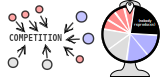
\includegraphics{images/roulette.png}

As can be seen, not all individual have the same size on the roulette
wheel. That depicts differences in their growth rates, biomass, or other
approximations of ``fitness''. Also, the roulette wheel contains an area
(shown in black) that shapes the chance that nobody reproduces. We will
try and implement this rule to let individuals reproduce based on their
fitness, but with only 10 competitors at a time. Let's start with a code
where individuals have a ``fitness'' value, but it not yet used for
selection (see below). \textbf{Read/test this code thoroughly before you
move on to the next section}.

\begin{tcolorbox}[enhanced jigsaw, bottomtitle=1mm, colback=white, leftrule=.75mm, rightrule=.15mm, left=2mm, toptitle=1mm, titlerule=0mm, breakable, coltitle=black, title=\textcolor{quarto-callout-note-color}{\faInfo}\hspace{0.5em}{CODE FOR ``fitness without fitness''}, opacityback=0, opacitybacktitle=0.6, bottomrule=.15mm, colbacktitle=quarto-callout-note-color!10!white, colframe=quarto-callout-note-color-frame, toprule=.15mm, arc=.35mm]

\begin{Shaded}
\begin{Highlighting}[]
\ImportTok{import}\NormalTok{ random}
\ImportTok{import}\NormalTok{ math}
\ImportTok{import}\NormalTok{ matplotlib.pyplot }\ImportTok{as}\NormalTok{ plt}

\CommentTok{\# Set the random number seed for reproducibility}
\NormalTok{random.seed(}\DecValTok{0}\NormalTok{)}

\NormalTok{plt.ion()  }\CommentTok{\# Enable interactive plotting}

\CommentTok{\# {-}{-}{-} PARAMETERS {-}{-}{-}}
\NormalTok{initial\_fitness }\OperatorTok{=} \FloatTok{0.1}            \CommentTok{\# Starting fitness for all individuals}
\NormalTok{population\_size }\OperatorTok{=} \DecValTok{500}             \CommentTok{\# Number of individuals (should be a square number for grid mode)}
\NormalTok{generations }\OperatorTok{=} \DecValTok{20000}               \CommentTok{\# Number of generations to simulate}
\NormalTok{mutation\_rate }\OperatorTok{=} \FloatTok{0.005}            \CommentTok{\# Probability of mutation per reproduction event}
\NormalTok{sample\_interval }\OperatorTok{=} \DecValTok{5}               \CommentTok{\# How often to sample and plot data}

\CommentTok{\# {-}{-}{-} INITIALIZATION {-}{-}{-}}
\CommentTok{\# Create initial population: all individuals start with the same fitness}
\NormalTok{population }\OperatorTok{=}\NormalTok{ [initial\_fitness }\ControlFlowTok{for}\NormalTok{ \_ }\KeywordTok{in} \BuiltInTok{range}\NormalTok{(population\_size)]}

\CommentTok{\# Lists to track average fitness and diversity over time}
\NormalTok{avg\_fitness }\OperatorTok{=}\NormalTok{ []}
\NormalTok{diversity\_over\_time }\OperatorTok{=}\NormalTok{ []}

\CommentTok{\# {-}{-}{-} CORE FUNCTIONS {-}{-}{-}}

\KeywordTok{def}\NormalTok{ mutate(fitness, rate}\OperatorTok{=}\NormalTok{mutation\_rate):}
    \CommentTok{"""Mutate the fitness value with a given probability."""}
    \ControlFlowTok{if}\NormalTok{ random.random() }\OperatorTok{\textless{}}\NormalTok{ rate:}
        \CommentTok{\# Fitness changes by a random value in [{-}0.1, 0.1], clipped to [0, 1]}
        \ControlFlowTok{return} \BuiltInTok{min}\NormalTok{(}\FloatTok{1.0}\NormalTok{, }\BuiltInTok{max}\NormalTok{(}\FloatTok{0.0}\NormalTok{, fitness }\OperatorTok{+}\NormalTok{ random.uniform(}\OperatorTok{{-}}\FloatTok{0.1}\NormalTok{, }\FloatTok{0.1}\NormalTok{)))}
    \ControlFlowTok{return}\NormalTok{ fitness}

\KeywordTok{def}\NormalTok{ calculate\_diversity(population):}
    \CommentTok{"""NOT YET IMPLEMENTED! Calculate diversity as the standard deviation of fitness values."""}
    \ControlFlowTok{return} \DecValTok{0} 

\CommentTok{\# {-}{-}{-} PLOTTING SETUP {-}{-}{-}}
\NormalTok{fig, ax1 }\OperatorTok{=}\NormalTok{ plt.subplots(figsize}\OperatorTok{=}\NormalTok{(}\DecValTok{12}\NormalTok{, }\DecValTok{8}\NormalTok{))}
\NormalTok{ax1.set\_xlabel(}\StringTok{"Generation"}\NormalTok{)}
\NormalTok{ax1.set\_ylabel(}\StringTok{"Average Fitness"}\NormalTok{, color}\OperatorTok{=}\StringTok{\textquotesingle{}tab:blue\textquotesingle{}}\NormalTok{)}
\NormalTok{ax1.set\_ylim(}\DecValTok{0}\NormalTok{, }\DecValTok{1}\NormalTok{)}
\NormalTok{line1, }\OperatorTok{=}\NormalTok{ ax1.plot([], [], color}\OperatorTok{=}\StringTok{\textquotesingle{}tab:blue\textquotesingle{}}\NormalTok{, linewidth}\OperatorTok{=}\DecValTok{2}\NormalTok{, label}\OperatorTok{=}\StringTok{\textquotesingle{}Fitness\textquotesingle{}}\NormalTok{)}
\NormalTok{ax1.tick\_params(axis}\OperatorTok{=}\StringTok{\textquotesingle{}y\textquotesingle{}}\NormalTok{, labelcolor}\OperatorTok{=}\StringTok{\textquotesingle{}tab:blue\textquotesingle{}}\NormalTok{)}

\CommentTok{\# Second y{-}axis for diversity}
\NormalTok{ax2 }\OperatorTok{=}\NormalTok{ ax1.twinx()}
\NormalTok{ax2.set\_ylabel(}\StringTok{"Diversity"}\NormalTok{, color}\OperatorTok{=}\StringTok{\textquotesingle{}tab:green\textquotesingle{}}\NormalTok{)}
\NormalTok{line2, }\OperatorTok{=}\NormalTok{ ax2.plot([], [], color}\OperatorTok{=}\StringTok{\textquotesingle{}tab:green\textquotesingle{}}\NormalTok{, linestyle}\OperatorTok{=}\StringTok{\textquotesingle{}:\textquotesingle{}}\NormalTok{, linewidth}\OperatorTok{=}\DecValTok{2}\NormalTok{, label}\OperatorTok{=}\StringTok{\textquotesingle{}Diversity\textquotesingle{}}\NormalTok{)}
\NormalTok{ax2.tick\_params(axis}\OperatorTok{=}\StringTok{\textquotesingle{}y\textquotesingle{}}\NormalTok{, labelcolor}\OperatorTok{=}\StringTok{\textquotesingle{}tab:green\textquotesingle{}}\NormalTok{)}

\NormalTok{fig.suptitle(}\StringTok{"Evolution Toward Fitness 1"}\NormalTok{)}
\NormalTok{fig.tight\_layout()}
\NormalTok{fig.legend(loc}\OperatorTok{=}\StringTok{\textquotesingle{}upper right\textquotesingle{}}\NormalTok{)}
\NormalTok{plt.grid(}\VariableTok{True}\NormalTok{)}
\NormalTok{plt.draw()}

\CommentTok{\# {-}{-}{-} EVOLUTION LOOP {-}{-}{-}}
\NormalTok{best\_fitness }\OperatorTok{=} \OperatorTok{{-}}\DecValTok{1}
\NormalTok{found }\OperatorTok{=} \VariableTok{False}

\ControlFlowTok{for}\NormalTok{ gen }\KeywordTok{in} \BuiltInTok{range}\NormalTok{(generations):}
\NormalTok{    total\_fit }\OperatorTok{=} \BuiltInTok{sum}\NormalTok{(population)}
\NormalTok{    best }\OperatorTok{=} \BuiltInTok{max}\NormalTok{(population)}
    \CommentTok{\# Print when a perfect solution is found}
    \ControlFlowTok{if}\NormalTok{ best }\OperatorTok{==} \DecValTok{1} \KeywordTok{and} \KeywordTok{not}\NormalTok{ found:}
\NormalTok{        found }\OperatorTok{=} \VariableTok{True}
        \BuiltInTok{print}\NormalTok{(}\StringTok{"Found perfect solution at generation"}\NormalTok{, gen)}
        
    \CommentTok{\# Sample and plot data at intervals}
    \ControlFlowTok{if}\NormalTok{ gen }\OperatorTok{\%}\NormalTok{ sample\_interval }\OperatorTok{==} \DecValTok{0}\NormalTok{:}
\NormalTok{        avg\_fitness.append(total\_fit }\OperatorTok{/}\NormalTok{ population\_size)}
\NormalTok{        diversity\_over\_time.append(calculate\_diversity(population))}
\NormalTok{        x\_vals }\OperatorTok{=}\NormalTok{ [i }\OperatorTok{*}\NormalTok{ sample\_interval }\ControlFlowTok{for}\NormalTok{ i }\KeywordTok{in} \BuiltInTok{range}\NormalTok{(}\BuiltInTok{len}\NormalTok{(avg\_fitness))]}
\NormalTok{        line1.set\_data(x\_vals, avg\_fitness)}
\NormalTok{        line2.set\_data(x\_vals, diversity\_over\_time)}
\NormalTok{        ax1.relim()}\OperatorTok{;}\NormalTok{ ax1.autoscale\_view()}
\NormalTok{        ax2.relim()}\OperatorTok{;}\NormalTok{ ax2.autoscale\_view()}
\NormalTok{        fig.suptitle(}\SpecialStringTok{f"Best Fitness: }\SpecialCharTok{\{}\NormalTok{best}\SpecialCharTok{:.2f\}}\SpecialStringTok{"}\NormalTok{, fontsize}\OperatorTok{=}\DecValTok{14}\NormalTok{)}
\NormalTok{        plt.pause(}\FloatTok{0.01}\NormalTok{)}
        

    \CommentTok{\# {-}{-}{-} MORAN PROCESS {-}{-}{-}}
    \CommentTok{\# For each individual, perform a reproduction event}
    \ControlFlowTok{for}\NormalTok{ \_ }\KeywordTok{in} \BuiltInTok{range}\NormalTok{(}\DecValTok{100}\NormalTok{):  }\CommentTok{\# 100 competition events per generation}
        \CommentTok{\# Select 1 random individual for replication}
\NormalTok{        probs }\OperatorTok{=}\NormalTok{ [}\DecValTok{1} \ControlFlowTok{for}\NormalTok{ fit }\KeywordTok{in}\NormalTok{ population] }\CommentTok{\# All probability weights are equal (1.0)}
\NormalTok{        parent\_idx }\OperatorTok{=}\NormalTok{ random.choices(}\BuiltInTok{range}\NormalTok{(}\BuiltInTok{len}\NormalTok{(population)), weights}\OperatorTok{=}\NormalTok{probs)[}\DecValTok{0}\NormalTok{] }\CommentTok{\# Grab one random individual based on an unweighted list...}
        \CommentTok{\# Select individual to be replaced (uniform random)}
\NormalTok{        dead\_idx }\OperatorTok{=}\NormalTok{ random.randrange(}\BuiltInTok{len}\NormalTok{(population))}
        \CommentTok{\# Copy population for next generation}
\NormalTok{        new\_pop }\OperatorTok{=}\NormalTok{ population.copy()}
        \CommentTok{\# Offspring replaces the dead individual (with possible mutation)}
\NormalTok{        new\_pop[dead\_idx] }\OperatorTok{=}\NormalTok{ mutate(population[parent\_idx])}
\NormalTok{        population }\OperatorTok{=}\NormalTok{ new\_pop}

\BuiltInTok{input}\NormalTok{(}\StringTok{"}\CharTok{\textbackslash{}n}\StringTok{Simulation complete. Press Enter to exit plot window..."}\NormalTok{)}
\end{Highlighting}
\end{Shaded}

\end{tcolorbox}

\section{Making a roulette wheel with everyone in
it}\label{making-a-roulette-wheel-with-everyone-in-it}

If you have read the code, you will see that we can pass a list of
weights to the function \texttt{random.choices}, to determine who is
most likely to be sampled. Currently, all the weights are set to 1:

\texttt{probs\ =\ {[}1\ for\ fit\ in\ population{]}\ \#\ All\ probability\ weights\ are\ equal\ (1.0)}

\begin{exercise}[Running the roulette wheel with fitness
values]\protect\hypertarget{exr-roulette}{}\label{exr-roulette}

\begin{enumerate}
\def\labelenumi{\alph{enumi}.}
\tightlist
\item
  Run the code with the current (all equal) weights. What happens?
\item
  Modify this line of code to take the fitness values as the weight,
  rather than 1. (hint: this is a VERY small change in the code).
\end{enumerate}

\end{exercise}

\section{A roulette wheel of a subset of
individuals}\label{a-roulette-wheel-of-a-subset-of-individuals}

Instead of letting everyone reproduce, let us modify the code to only
sample from a smaller list of `competitors', and spin a virtual roulette
wheel to determine who wins. There are many ways to implement this, but
here's how we will do it. We will sample \(N\) individuals from the
population, and implement the following algorithm:

\begin{enumerate}
\def\labelenumi{\arabic{enumi}.}
\tightlist
\item
  Select a random subset of \(N\) individuals from the population.
\item
  Take/compute the fitness of each selected individual.
\item
  Add a reproduction-skip option with a fixed weight.
\item
  Choose one individual or the skip option using weighted random
  selection.
\item
  If an individual was chosen, mutate it and replace a random individual
  in the population.
\end{enumerate}

Below, there's a small snippet of code doing what is explained
above\footnote{Note that this is from the full code, so this code does
  not work stand-alone}. The variable \texttt{no\_reproduction\_chance}
is the fixed weight that nobody gets to reproduce:

\begin{tcolorbox}[enhanced jigsaw, bottomtitle=1mm, colback=white, leftrule=.75mm, rightrule=.15mm, left=2mm, toptitle=1mm, titlerule=0mm, breakable, coltitle=black, title=\textcolor{quarto-callout-note-color}{\faInfo}\hspace{0.5em}{Roulette wheel algorithm}, opacityback=0, opacitybacktitle=0.6, bottomrule=.15mm, colbacktitle=quarto-callout-note-color!10!white, colframe=quarto-callout-note-color-frame, toprule=.15mm, arc=.35mm]

\begin{Shaded}
\begin{Highlighting}[]
\NormalTok{  tournament\_size }\OperatorTok{=} \DecValTok{10}  
\NormalTok{  no\_reproduction\_chance }\OperatorTok{=} \DecValTok{1}
  
\NormalTok{  competitors }\OperatorTok{=}\NormalTok{ random.sample(population, tournament\_size)}
  \CommentTok{\# Make a list of their fitness values}
\NormalTok{  fitness\_values }\OperatorTok{=}\NormalTok{ [fit }\ControlFlowTok{for}\NormalTok{ fit }\KeywordTok{in}\NormalTok{ competitors]}
\NormalTok{  total }\OperatorTok{=} \BuiltInTok{sum}\NormalTok{(fitness\_values)}
  \CommentTok{\# Add a "no reproduction" dummy competitor with fitness = 0}
\NormalTok{  competitors\_with\_dummy }\OperatorTok{=}\NormalTok{ competitors }\OperatorTok{+}\NormalTok{ [}\VariableTok{None}\NormalTok{]}
\NormalTok{  probs }\OperatorTok{=}\NormalTok{ [f }\OperatorTok{/}\NormalTok{ total }\ControlFlowTok{for}\NormalTok{ f }\KeywordTok{in}\NormalTok{ fitness\_values] }\OperatorTok{+}\NormalTok{ [no\_reproduction\_chance]}
\NormalTok{  winner }\OperatorTok{=}\NormalTok{ random.choices(competitors\_with\_dummy, weights}\OperatorTok{=}\NormalTok{probs, k}\OperatorTok{=}\DecValTok{1}\NormalTok{)[}\DecValTok{0}\NormalTok{]}
  \ControlFlowTok{if}\NormalTok{ winner }\KeywordTok{is} \KeywordTok{not} \VariableTok{None}\NormalTok{:}
      \CommentTok{\# Mutate winner to produce offspring}
\NormalTok{      offspring }\OperatorTok{=}\NormalTok{ mutate(winner)}
\NormalTok{      remove\_idx }\OperatorTok{=}\NormalTok{ random.randrange(}\BuiltInTok{len}\NormalTok{(population))}
\NormalTok{      population[remove\_idx] }\OperatorTok{=}\NormalTok{ offspring  }
        
\end{Highlighting}
\end{Shaded}

\end{tcolorbox}

After you understand the roulette wheel algorithm, do the following
exercise:

\begin{exercise}[Questions about the roulette wheel - Algorithmic
thinking]\protect\hypertarget{exr-roulette}{}\label{exr-roulette}

\begin{enumerate}
\def\labelenumi{\alph{enumi}.}
\tightlist
\item
  Let's imagine a moment where the roulette wheel contains only 10
  highly unfit individuals (e.g.~all fitness values are 0.01). What is
  the chance that someone will reproduce? (you don't have to calculate
  it, but give your reasoning)
\item
  Answer the same question as in \textbf{a.}, but now imagine that all
  10 individuals have a fitness value of 1.
\item
  Answer question b. and c.~again, but now assume that
  \texttt{no\_reproduction\_chance} is equal to 0.
\item
  Describe what the \texttt{no\_reproduction\_chance} parameter does in
  biological terms.
\item
  Spatially structured populations are often placed on a grid.
  \textbf{Describe} how you could implement a roulette wheel to resolve
  \emph{local} competition, \emph{e.g.} when an empty grid point is
  competed for by the neighbours.
\end{enumerate}

\end{exercise}

\section{Diversity patterns}\label{diversity-patterns}

Modify the function \texttt{calculate\_diversity} to calculate the
diversity of the population as the standard deviation of the fitness
values.

\begin{exercise}[The dynamics of diversity -
Biology]\protect\hypertarget{exr-diversitydynamics}{}\label{exr-diversitydynamics}

\begin{enumerate}
\def\labelenumi{\alph{enumi}.}
\tightlist
\item
  Use a low mutation rate and study the dynamics of diversity. Describe
  the pattern verbally.
\end{enumerate}

\end{exercise}

\section{Evolving a DNA sequence}\label{evolving-a-dna-sequence}

A big problem with the previous model is there is no true distinction
between genotype (that which mutates) and phenotype (that which is
selected). Let us try and adapt the model to be more biologically
meaningful, by making each individual represented by a DNA sequence.
Copy the following code:

\begin{tcolorbox}[enhanced jigsaw, bottomtitle=1mm, colback=white, leftrule=.75mm, rightrule=.15mm, left=2mm, toptitle=1mm, titlerule=0mm, breakable, coltitle=black, title=\textcolor{quarto-callout-note-color}{\faInfo}\hspace{0.5em}{Starting code for ``evolving a DNA sequence''}, opacityback=0, opacitybacktitle=0.6, bottomrule=.15mm, colbacktitle=quarto-callout-note-color!10!white, colframe=quarto-callout-note-color-frame, toprule=.15mm, arc=.35mm]

\begin{Shaded}
\begin{Highlighting}[]
\ImportTok{import}\NormalTok{ random}
\ImportTok{import}\NormalTok{ math}
\ImportTok{import}\NormalTok{ matplotlib.pyplot }\ImportTok{as}\NormalTok{ plt}
\ImportTok{from}\NormalTok{ collections }\ImportTok{import}\NormalTok{ Counter}

\CommentTok{\# set the random number seed}
\NormalTok{random.seed(}\DecValTok{0}\NormalTok{)}

\NormalTok{plt.ion()  }\CommentTok{\# Enable interactive mode}

\CommentTok{\# Parameters}
\NormalTok{alphabet }\OperatorTok{=} \StringTok{"ATCG"}
\NormalTok{target\_sequence }\OperatorTok{=} \StringTok{"GATGCGCGCTGGATTAAC"}  \CommentTok{\# Example target sequence}
\NormalTok{dna\_length }\OperatorTok{=} \BuiltInTok{len}\NormalTok{(target\_sequence)}
\NormalTok{target\_length }\OperatorTok{=} \BuiltInTok{len}\NormalTok{(target\_sequence)}

\CommentTok{\# Simulation settings}
\NormalTok{population\_size }\OperatorTok{=} \DecValTok{500}  \CommentTok{\# must be a square number for grid mode}
\NormalTok{generations }\OperatorTok{=} \DecValTok{20000}
\NormalTok{mutation\_rate }\OperatorTok{=} \FloatTok{0.001}
\NormalTok{sample\_interval }\OperatorTok{=} \DecValTok{5}
\NormalTok{sample\_size }\OperatorTok{=}\NormalTok{ population\_size}
\NormalTok{no\_reproduction\_chance }\OperatorTok{=} \FloatTok{0.1}

\CommentTok{\# Core functions}
\KeywordTok{def}\NormalTok{ fitness(dna):}
    \ControlFlowTok{return} \DecValTok{1} \OperatorTok{{-}} \BuiltInTok{sum}\NormalTok{(a }\OperatorTok{!=}\NormalTok{ b }\ControlFlowTok{for}\NormalTok{ a, b }\KeywordTok{in} \BuiltInTok{zip}\NormalTok{(dna, target\_sequence)) }\OperatorTok{/}\NormalTok{ target\_length}

\KeywordTok{def}\NormalTok{ mutate(dna, rate}\OperatorTok{=}\NormalTok{mutation\_rate):}
    \ControlFlowTok{return} \StringTok{\textquotesingle{}\textquotesingle{}}\NormalTok{.join(}
\NormalTok{        random.choice([b }\ControlFlowTok{for}\NormalTok{ b }\KeywordTok{in}\NormalTok{ alphabet }\ControlFlowTok{if}\NormalTok{ b }\OperatorTok{!=}\NormalTok{ base]) }\ControlFlowTok{if}\NormalTok{ random.random() }\OperatorTok{\textless{}}\NormalTok{ rate }\ControlFlowTok{else}\NormalTok{ base}
        \ControlFlowTok{for}\NormalTok{ base }\KeywordTok{in}\NormalTok{ dna}
\NormalTok{    )}

\KeywordTok{def}\NormalTok{ count\_beneficial\_mutations(dna):}
\NormalTok{    f0 }\OperatorTok{=}\NormalTok{ fitness(dna)}
\NormalTok{    count }\OperatorTok{=} \DecValTok{0}
    \ControlFlowTok{for}\NormalTok{ i }\KeywordTok{in} \BuiltInTok{range}\NormalTok{(}\BuiltInTok{len}\NormalTok{(dna)):}
        \ControlFlowTok{for}\NormalTok{ b }\KeywordTok{in}\NormalTok{ alphabet:}
            \ControlFlowTok{if}\NormalTok{ b }\OperatorTok{!=}\NormalTok{ dna[i]:}
\NormalTok{                mutant }\OperatorTok{=}\NormalTok{ dna[:i] }\OperatorTok{+}\NormalTok{ b }\OperatorTok{+}\NormalTok{ dna[i}\OperatorTok{+}\DecValTok{1}\NormalTok{:]}
                \ControlFlowTok{if}\NormalTok{ fitness(mutant) }\OperatorTok{\textgreater{}}\NormalTok{ f0:}
\NormalTok{                    count }\OperatorTok{+=} \DecValTok{1}
    \ControlFlowTok{return}\NormalTok{ count}

\KeywordTok{def}\NormalTok{ diversity(pop):}
\NormalTok{    counts }\OperatorTok{=}\NormalTok{ \{\}}
    \ControlFlowTok{for}\NormalTok{ ind }\KeywordTok{in}\NormalTok{ pop:}
\NormalTok{        counts[ind] }\OperatorTok{=}\NormalTok{ counts.get(ind, }\DecValTok{0}\NormalTok{) }\OperatorTok{+} \DecValTok{1}
\NormalTok{    total }\OperatorTok{=} \BuiltInTok{len}\NormalTok{(pop)}
    \ControlFlowTok{return} \OperatorTok{{-}}\BuiltInTok{sum}\NormalTok{((c}\OperatorTok{/}\NormalTok{total) }\OperatorTok{*}\NormalTok{ math.log(c}\OperatorTok{/}\NormalTok{total }\OperatorTok{+} \FloatTok{1e{-}9}\NormalTok{) }\ControlFlowTok{for}\NormalTok{ c }\KeywordTok{in}\NormalTok{ counts.values()) }\ControlFlowTok{if}\NormalTok{ total }\OperatorTok{\textgreater{}} \DecValTok{0} \ControlFlowTok{else} \DecValTok{0}

\CommentTok{\# Initialize population}
\NormalTok{initial\_sequence }\OperatorTok{=} \StringTok{"GATAGCGAAGTTTAGCCG"} \CommentTok{\# far from target (only first 3 are correct)}
\NormalTok{population }\OperatorTok{=}\NormalTok{ [initial\_sequence }\ControlFlowTok{for}\NormalTok{ \_ }\KeywordTok{in} \BuiltInTok{range}\NormalTok{(population\_size)]}

\NormalTok{avg\_fitness }\OperatorTok{=}\NormalTok{ []}
\NormalTok{avg\_beneficial }\OperatorTok{=}\NormalTok{ []}
\NormalTok{diversity\_over\_time }\OperatorTok{=}\NormalTok{ []}
\NormalTok{best\_individuals }\OperatorTok{=}\NormalTok{ []}

\KeywordTok{def}\NormalTok{ get\_neighbors(i, j):}
    \ControlFlowTok{return}\NormalTok{ [(x }\OperatorTok{\%}\NormalTok{ side, y }\OperatorTok{\%}\NormalTok{ side)}
            \ControlFlowTok{for}\NormalTok{ x }\KeywordTok{in} \BuiltInTok{range}\NormalTok{(i}\OperatorTok{{-}}\DecValTok{1}\NormalTok{, i}\OperatorTok{+}\DecValTok{2}\NormalTok{)}
            \ControlFlowTok{for}\NormalTok{ y }\KeywordTok{in} \BuiltInTok{range}\NormalTok{(j}\OperatorTok{{-}}\DecValTok{1}\NormalTok{, j}\OperatorTok{+}\DecValTok{2}\NormalTok{)]}

\CommentTok{\# Initialize interactive plot}
\NormalTok{fig, ax1 }\OperatorTok{=}\NormalTok{ plt.subplots(figsize}\OperatorTok{=}\NormalTok{(}\DecValTok{12}\NormalTok{, }\DecValTok{8}\NormalTok{))}
\NormalTok{ax1.set\_xlabel(}\StringTok{"Generation"}\NormalTok{)}
\NormalTok{ax1.set\_ylabel(}\StringTok{"Average Fitness"}\NormalTok{, color}\OperatorTok{=}\StringTok{\textquotesingle{}tab:blue\textquotesingle{}}\NormalTok{)}
\NormalTok{ax1.set\_ylim(}\DecValTok{0}\NormalTok{, }\DecValTok{1}\NormalTok{)}
\NormalTok{line1, }\OperatorTok{=}\NormalTok{ ax1.plot([], [], color}\OperatorTok{=}\StringTok{\textquotesingle{}tab:blue\textquotesingle{}}\NormalTok{, linewidth}\OperatorTok{=}\DecValTok{2}\NormalTok{, label}\OperatorTok{=}\StringTok{\textquotesingle{}Fitness\textquotesingle{}}\NormalTok{)}
\NormalTok{ax1.tick\_params(axis}\OperatorTok{=}\StringTok{\textquotesingle{}y\textquotesingle{}}\NormalTok{, labelcolor}\OperatorTok{=}\StringTok{\textquotesingle{}tab:blue\textquotesingle{}}\NormalTok{)}

\NormalTok{ax2 }\OperatorTok{=}\NormalTok{ ax1.twinx()}
\NormalTok{ax2.set\_ylabel(}\StringTok{"Beneficial Mutations / Diversity"}\NormalTok{, color}\OperatorTok{=}\StringTok{\textquotesingle{}tab:purple\textquotesingle{}}\NormalTok{)}
\NormalTok{line2, }\OperatorTok{=}\NormalTok{ ax2.plot([], [], color}\OperatorTok{=}\StringTok{\textquotesingle{}tab:purple\textquotesingle{}}\NormalTok{, linestyle}\OperatorTok{=}\StringTok{\textquotesingle{}{-}{-}\textquotesingle{}}\NormalTok{, linewidth}\OperatorTok{=}\DecValTok{2}\NormalTok{, label}\OperatorTok{=}\StringTok{\textquotesingle{}Beneficial Mutations\textquotesingle{}}\NormalTok{)}
\NormalTok{line3, }\OperatorTok{=}\NormalTok{ ax2.plot([], [], color}\OperatorTok{=}\StringTok{\textquotesingle{}tab:green\textquotesingle{}}\NormalTok{, linestyle}\OperatorTok{=}\StringTok{\textquotesingle{}:\textquotesingle{}}\NormalTok{, linewidth}\OperatorTok{=}\DecValTok{2}\NormalTok{, label}\OperatorTok{=}\StringTok{\textquotesingle{}Diversity\textquotesingle{}}\NormalTok{)}
\NormalTok{ax2.tick\_params(axis}\OperatorTok{=}\StringTok{\textquotesingle{}y\textquotesingle{}}\NormalTok{, labelcolor}\OperatorTok{=}\StringTok{\textquotesingle{}tab:purple\textquotesingle{}}\NormalTok{)}
\NormalTok{fig.suptitle(}\StringTok{"Evolution Toward Target Sequence"}\NormalTok{)}
\NormalTok{fig.tight\_layout()}
\NormalTok{ax2.set\_ylim(}\DecValTok{0}\NormalTok{, }\DecValTok{20}\NormalTok{)}
\NormalTok{fig.legend(loc}\OperatorTok{=}\StringTok{\textquotesingle{}upper right\textquotesingle{}}\NormalTok{)}
\NormalTok{plt.grid(}\VariableTok{True}\NormalTok{)}
\NormalTok{plt.draw()}

\NormalTok{best\_seq }\OperatorTok{=} \StringTok{""}
\NormalTok{best\_score }\OperatorTok{=} \OperatorTok{{-}}\DecValTok{1}
\NormalTok{found }\OperatorTok{=} \VariableTok{False}

\CommentTok{\# Evolution loop}
\ControlFlowTok{for}\NormalTok{ gen }\KeywordTok{in} \BuiltInTok{range}\NormalTok{(generations):}
\NormalTok{    fitnesses }\OperatorTok{=}\NormalTok{ [fitness(ind) }\ControlFlowTok{for}\NormalTok{ ind }\KeywordTok{in}\NormalTok{ population]}
\NormalTok{    total\_fit }\OperatorTok{=} \BuiltInTok{sum}\NormalTok{(fitnesses)}
\NormalTok{    best }\OperatorTok{=} \BuiltInTok{max}\NormalTok{(fitnesses)}
    \ControlFlowTok{if}\NormalTok{(best }\OperatorTok{==} \DecValTok{1} \KeywordTok{and} \KeywordTok{not}\NormalTok{ found):}
\NormalTok{        found }\OperatorTok{=} \VariableTok{True}
        \BuiltInTok{print}\NormalTok{(}\StringTok{"Found perfect solution at generation"}\NormalTok{, gen)}
        
    \ControlFlowTok{if}\NormalTok{ gen }\OperatorTok{\%}\NormalTok{ sample\_interval }\OperatorTok{==} \DecValTok{0}\NormalTok{:}
\NormalTok{        sample }\OperatorTok{=}\NormalTok{ random.sample(population, sample\_size)}
\NormalTok{        avg\_beneficial.append(}\BuiltInTok{sum}\NormalTok{(count\_beneficial\_mutations(ind) }\ControlFlowTok{for}\NormalTok{ ind }\KeywordTok{in}\NormalTok{ sample) }\OperatorTok{/}\NormalTok{ sample\_size)}
\NormalTok{        diversity\_over\_time.append(diversity(population))}

        \CommentTok{\# Update plot data}
\NormalTok{        line1.set\_data(}\BuiltInTok{range}\NormalTok{(}\BuiltInTok{len}\NormalTok{(avg\_fitness)}\OperatorTok{+}\DecValTok{1}\NormalTok{), avg\_fitness }\OperatorTok{+}\NormalTok{ [}\BuiltInTok{sum}\NormalTok{(fitnesses)}\OperatorTok{/}\NormalTok{population\_size])}
\NormalTok{        line2.set\_data(}\BuiltInTok{range}\NormalTok{(}\BuiltInTok{len}\NormalTok{(avg\_beneficial)), avg\_beneficial)}
\NormalTok{        line3.set\_data(}\BuiltInTok{range}\NormalTok{(}\BuiltInTok{len}\NormalTok{(diversity\_over\_time)), diversity\_over\_time)}
\NormalTok{        ax1.relim()}\OperatorTok{;}\NormalTok{ ax1.autoscale\_view()}
\NormalTok{        ax2.relim()}\OperatorTok{;}\NormalTok{ ax2.autoscale\_view()}
\NormalTok{        best }\OperatorTok{=} \BuiltInTok{max}\NormalTok{(population, key}\OperatorTok{=}\NormalTok{fitness)}
\NormalTok{        fig.suptitle(}\SpecialStringTok{f"Best: }\SpecialCharTok{\{}\NormalTok{best}\SpecialCharTok{\}}\SpecialStringTok{ (target: }\SpecialCharTok{\{}\NormalTok{target\_sequence}\SpecialCharTok{\}}\SpecialStringTok{)"}\NormalTok{, fontsize}\OperatorTok{=}\DecValTok{14}\NormalTok{)}
\NormalTok{        plt.pause(}\FloatTok{0.01}\NormalTok{)}

    \ControlFlowTok{else}\NormalTok{:}
\NormalTok{        avg\_beneficial.append(avg\_beneficial[}\OperatorTok{{-}}\DecValTok{1}\NormalTok{])}
\NormalTok{        diversity\_over\_time.append(diversity\_over\_time[}\OperatorTok{{-}}\DecValTok{1}\NormalTok{])}

    \CommentTok{\# Tournament selection (as in evolving\_fitness\_final.py)}
\NormalTok{    new\_pop }\OperatorTok{=}\NormalTok{ []}
\NormalTok{    tournament\_size }\OperatorTok{=} \DecValTok{10}  \CommentTok{\# can be adjusted}

    \ControlFlowTok{for}\NormalTok{ \_ }\KeywordTok{in} \BuiltInTok{range}\NormalTok{(population\_size):}
        \CommentTok{\# Select tournament\_size individuals randomly}
\NormalTok{        competitors }\OperatorTok{=}\NormalTok{ random.sample(population, tournament\_size)}
        \CommentTok{\# Pick the one with highest fitness}
\NormalTok{        fitness\_values }\OperatorTok{=}\NormalTok{ [fitness(ind) }\ControlFlowTok{for}\NormalTok{ ind }\KeywordTok{in}\NormalTok{ competitors]}
\NormalTok{        total }\OperatorTok{=} \BuiltInTok{sum}\NormalTok{(fitness\_values)}
        
\NormalTok{        probs }\OperatorTok{=}\NormalTok{ [f }\OperatorTok{/}\NormalTok{ total }\ControlFlowTok{for}\NormalTok{ f }\KeywordTok{in}\NormalTok{ fitness\_values]}
\NormalTok{        winner }\OperatorTok{=}\NormalTok{ random.choices(competitors, weights}\OperatorTok{=}\NormalTok{probs, k}\OperatorTok{=}\DecValTok{1}\NormalTok{)[}\DecValTok{0}\NormalTok{]}
        \CommentTok{\# Mutate winner to produce offspring}
\NormalTok{        offspring }\OperatorTok{=}\NormalTok{ mutate(winner)}
\NormalTok{        new\_pop.append(offspring)}

\NormalTok{    population }\OperatorTok{=}\NormalTok{ new\_pop}

\NormalTok{    avg\_fitness.append(}\BuiltInTok{sum}\NormalTok{(fitness(ind) }\ControlFlowTok{for}\NormalTok{ ind }\KeywordTok{in}\NormalTok{ population) }\OperatorTok{/}\NormalTok{ population\_size)}
    \ControlFlowTok{if}\NormalTok{ gen }\OperatorTok{\%} \DecValTok{250} \OperatorTok{==} \DecValTok{0}\NormalTok{:}
\NormalTok{        best }\OperatorTok{=} \BuiltInTok{max}\NormalTok{(population, key}\OperatorTok{=}\NormalTok{fitness)}
\NormalTok{        best\_individuals.append((gen, best))}

\BuiltInTok{input}\NormalTok{(}\StringTok{"}\CharTok{\textbackslash{}n}\StringTok{Simulation complete. Press Enter to exit plot window..."}\NormalTok{)}
\end{Highlighting}
\end{Shaded}

\end{tcolorbox}

Answer the following questions using the options available in the model:

\begin{exercise}[Evolving DNA - Biology / abstract
thinking]\protect\hypertarget{exr-evolving-dna}{}\label{exr-evolving-dna}

~

\begin{enumerate}
\def\labelenumi{\alph{enumi}.}
\tightlist
\item
  Run the code. What does the new (dashed blue) line represent? Do you
  understand how it changes over time?
\end{enumerate}

The program reports after how many generations it manages to find the
target sequence. With default settings this can take a long time\ldots{}
(default: 429 generations)

\begin{enumerate}
\def\labelenumi{\alph{enumi}.}
\setcounter{enumi}{1}
\tightlist
\item
  Modify the mutation rate to see how it affects the time to find the
  target sequence. Try different mutation rates between 0.0001 and 0.1.
  Keep track of both how long (number of generations) it takes to find
  the target, and how fit the population is once the target is found.
  What do you observe?
\item
  Diversity is no longer calculated as the standard deviation in
  fitness, but as the Shannon diversity of all present sequences
  (although it is not super complex, you do not need to fully understand
  this function). Because of this, the exact number (quantities) cannot
  be compared to our earlier model. Do you see a \emph{qualitative}
  differences?
\item
  Study how fitness is calculated in this model. Is there a distinction
  between genotype en phenotype? Why/why not?
\end{enumerate}

\end{exercise}

\section{Evolving a protein sequence}\label{evolving-a-protein-sequence}

Next we will extend the simulation a little more. The individual
genotypes will still be represented as a DNA sequence, but before
evaluating fitness this will be translated into a \textbf{protein}
sequence. To do so, the code first defines the codon table (which we of
course all know by heart =)), and then translates the DNA sequence into
a protein sequence. The protein sequence is then used to calculate the
fitness of the individual, which is based on how well the protein
sequence matches a target protein sequence. The code is as follows:

\begin{tcolorbox}[enhanced jigsaw, bottomtitle=1mm, colback=white, leftrule=.75mm, rightrule=.15mm, left=2mm, toptitle=1mm, titlerule=0mm, breakable, coltitle=black, title=\textcolor{quarto-callout-note-color}{\faInfo}\hspace{0.5em}{Starting code for evolving a protein sequence}, opacityback=0, opacitybacktitle=0.6, bottomrule=.15mm, colbacktitle=quarto-callout-note-color!10!white, colframe=quarto-callout-note-color-frame, toprule=.15mm, arc=.35mm]

\begin{Shaded}
\begin{Highlighting}[]
\ImportTok{import}\NormalTok{ random}
\ImportTok{import}\NormalTok{ math}
\ImportTok{import}\NormalTok{ matplotlib.pyplot }\ImportTok{as}\NormalTok{ plt}
\ImportTok{from}\NormalTok{ collections }\ImportTok{import}\NormalTok{ Counter}

\CommentTok{\# set the random number seed}
\NormalTok{random.seed(}\DecValTok{0}\NormalTok{)}

\NormalTok{plt.ion()  }\CommentTok{\# Enable interactive mode}

\CommentTok{\# Codon table}
\NormalTok{codon\_table }\OperatorTok{=}\NormalTok{ \{}
    \StringTok{\textquotesingle{}TTT\textquotesingle{}}\NormalTok{: }\StringTok{\textquotesingle{}F\textquotesingle{}}\NormalTok{, }\StringTok{\textquotesingle{}TTC\textquotesingle{}}\NormalTok{: }\StringTok{\textquotesingle{}F\textquotesingle{}}\NormalTok{, }\StringTok{\textquotesingle{}TTA\textquotesingle{}}\NormalTok{: }\StringTok{\textquotesingle{}L\textquotesingle{}}\NormalTok{, }\StringTok{\textquotesingle{}TTG\textquotesingle{}}\NormalTok{: }\StringTok{\textquotesingle{}L\textquotesingle{}}\NormalTok{, }\StringTok{\textquotesingle{}CTT\textquotesingle{}}\NormalTok{: }\StringTok{\textquotesingle{}L\textquotesingle{}}\NormalTok{, }\StringTok{\textquotesingle{}CTC\textquotesingle{}}\NormalTok{: }\StringTok{\textquotesingle{}L\textquotesingle{}}\NormalTok{, }\StringTok{\textquotesingle{}CTA\textquotesingle{}}\NormalTok{: }\StringTok{\textquotesingle{}L\textquotesingle{}}\NormalTok{, }\StringTok{\textquotesingle{}CTG\textquotesingle{}}\NormalTok{: }\StringTok{\textquotesingle{}L\textquotesingle{}}\NormalTok{,}
    \StringTok{\textquotesingle{}ATT\textquotesingle{}}\NormalTok{: }\StringTok{\textquotesingle{}I\textquotesingle{}}\NormalTok{, }\StringTok{\textquotesingle{}ATC\textquotesingle{}}\NormalTok{: }\StringTok{\textquotesingle{}I\textquotesingle{}}\NormalTok{, }\StringTok{\textquotesingle{}ATA\textquotesingle{}}\NormalTok{: }\StringTok{\textquotesingle{}I\textquotesingle{}}\NormalTok{, }\StringTok{\textquotesingle{}ATG\textquotesingle{}}\NormalTok{: }\StringTok{\textquotesingle{}M\textquotesingle{}}\NormalTok{,}
    \StringTok{\textquotesingle{}GTT\textquotesingle{}}\NormalTok{: }\StringTok{\textquotesingle{}V\textquotesingle{}}\NormalTok{, }\StringTok{\textquotesingle{}GTC\textquotesingle{}}\NormalTok{: }\StringTok{\textquotesingle{}V\textquotesingle{}}\NormalTok{, }\StringTok{\textquotesingle{}GTA\textquotesingle{}}\NormalTok{: }\StringTok{\textquotesingle{}V\textquotesingle{}}\NormalTok{, }\StringTok{\textquotesingle{}GTG\textquotesingle{}}\NormalTok{: }\StringTok{\textquotesingle{}V\textquotesingle{}}\NormalTok{,}
    \StringTok{\textquotesingle{}TCT\textquotesingle{}}\NormalTok{: }\StringTok{\textquotesingle{}S\textquotesingle{}}\NormalTok{, }\StringTok{\textquotesingle{}TCC\textquotesingle{}}\NormalTok{: }\StringTok{\textquotesingle{}S\textquotesingle{}}\NormalTok{, }\StringTok{\textquotesingle{}TCA\textquotesingle{}}\NormalTok{: }\StringTok{\textquotesingle{}S\textquotesingle{}}\NormalTok{, }\StringTok{\textquotesingle{}TCG\textquotesingle{}}\NormalTok{: }\StringTok{\textquotesingle{}S\textquotesingle{}}\NormalTok{, }\StringTok{\textquotesingle{}AGT\textquotesingle{}}\NormalTok{: }\StringTok{\textquotesingle{}S\textquotesingle{}}\NormalTok{, }\StringTok{\textquotesingle{}AGC\textquotesingle{}}\NormalTok{: }\StringTok{\textquotesingle{}S\textquotesingle{}}\NormalTok{,}
    \StringTok{\textquotesingle{}CCT\textquotesingle{}}\NormalTok{: }\StringTok{\textquotesingle{}P\textquotesingle{}}\NormalTok{, }\StringTok{\textquotesingle{}CCC\textquotesingle{}}\NormalTok{: }\StringTok{\textquotesingle{}P\textquotesingle{}}\NormalTok{, }\StringTok{\textquotesingle{}CCA\textquotesingle{}}\NormalTok{: }\StringTok{\textquotesingle{}P\textquotesingle{}}\NormalTok{, }\StringTok{\textquotesingle{}CCG\textquotesingle{}}\NormalTok{: }\StringTok{\textquotesingle{}P\textquotesingle{}}\NormalTok{,}
    \StringTok{\textquotesingle{}ACT\textquotesingle{}}\NormalTok{: }\StringTok{\textquotesingle{}T\textquotesingle{}}\NormalTok{, }\StringTok{\textquotesingle{}ACC\textquotesingle{}}\NormalTok{: }\StringTok{\textquotesingle{}T\textquotesingle{}}\NormalTok{, }\StringTok{\textquotesingle{}ACA\textquotesingle{}}\NormalTok{: }\StringTok{\textquotesingle{}T\textquotesingle{}}\NormalTok{, }\StringTok{\textquotesingle{}ACG\textquotesingle{}}\NormalTok{: }\StringTok{\textquotesingle{}T\textquotesingle{}}\NormalTok{,}
    \StringTok{\textquotesingle{}GCT\textquotesingle{}}\NormalTok{: }\StringTok{\textquotesingle{}A\textquotesingle{}}\NormalTok{, }\StringTok{\textquotesingle{}GCC\textquotesingle{}}\NormalTok{: }\StringTok{\textquotesingle{}A\textquotesingle{}}\NormalTok{, }\StringTok{\textquotesingle{}GCA\textquotesingle{}}\NormalTok{: }\StringTok{\textquotesingle{}A\textquotesingle{}}\NormalTok{, }\StringTok{\textquotesingle{}GCG\textquotesingle{}}\NormalTok{: }\StringTok{\textquotesingle{}A\textquotesingle{}}\NormalTok{,}
    \StringTok{\textquotesingle{}TAT\textquotesingle{}}\NormalTok{: }\StringTok{\textquotesingle{}Y\textquotesingle{}}\NormalTok{, }\StringTok{\textquotesingle{}TAC\textquotesingle{}}\NormalTok{: }\StringTok{\textquotesingle{}Y\textquotesingle{}}\NormalTok{, }\StringTok{\textquotesingle{}CAT\textquotesingle{}}\NormalTok{: }\StringTok{\textquotesingle{}H\textquotesingle{}}\NormalTok{, }\StringTok{\textquotesingle{}CAC\textquotesingle{}}\NormalTok{: }\StringTok{\textquotesingle{}H\textquotesingle{}}\NormalTok{,}
    \StringTok{\textquotesingle{}CAA\textquotesingle{}}\NormalTok{: }\StringTok{\textquotesingle{}Q\textquotesingle{}}\NormalTok{, }\StringTok{\textquotesingle{}CAG\textquotesingle{}}\NormalTok{: }\StringTok{\textquotesingle{}Q\textquotesingle{}}\NormalTok{, }\StringTok{\textquotesingle{}AAT\textquotesingle{}}\NormalTok{: }\StringTok{\textquotesingle{}N\textquotesingle{}}\NormalTok{, }\StringTok{\textquotesingle{}AAC\textquotesingle{}}\NormalTok{: }\StringTok{\textquotesingle{}N\textquotesingle{}}\NormalTok{,}
    \StringTok{\textquotesingle{}AAA\textquotesingle{}}\NormalTok{: }\StringTok{\textquotesingle{}K\textquotesingle{}}\NormalTok{, }\StringTok{\textquotesingle{}AAG\textquotesingle{}}\NormalTok{: }\StringTok{\textquotesingle{}K\textquotesingle{}}\NormalTok{, }\StringTok{\textquotesingle{}GAT\textquotesingle{}}\NormalTok{: }\StringTok{\textquotesingle{}D\textquotesingle{}}\NormalTok{, }\StringTok{\textquotesingle{}GAC\textquotesingle{}}\NormalTok{: }\StringTok{\textquotesingle{}D\textquotesingle{}}\NormalTok{,}
    \StringTok{\textquotesingle{}GAA\textquotesingle{}}\NormalTok{: }\StringTok{\textquotesingle{}E\textquotesingle{}}\NormalTok{, }\StringTok{\textquotesingle{}GAG\textquotesingle{}}\NormalTok{: }\StringTok{\textquotesingle{}E\textquotesingle{}}\NormalTok{, }\StringTok{\textquotesingle{}TGT\textquotesingle{}}\NormalTok{: }\StringTok{\textquotesingle{}C\textquotesingle{}}\NormalTok{, }\StringTok{\textquotesingle{}TGC\textquotesingle{}}\NormalTok{: }\StringTok{\textquotesingle{}C\textquotesingle{}}\NormalTok{,}
    \StringTok{\textquotesingle{}TGG\textquotesingle{}}\NormalTok{: }\StringTok{\textquotesingle{}W\textquotesingle{}}\NormalTok{, }\StringTok{\textquotesingle{}CGT\textquotesingle{}}\NormalTok{: }\StringTok{\textquotesingle{}R\textquotesingle{}}\NormalTok{, }\StringTok{\textquotesingle{}CGC\textquotesingle{}}\NormalTok{: }\StringTok{\textquotesingle{}R\textquotesingle{}}\NormalTok{, }\StringTok{\textquotesingle{}CGA\textquotesingle{}}\NormalTok{: }\StringTok{\textquotesingle{}R\textquotesingle{}}\NormalTok{, }\StringTok{\textquotesingle{}CGG\textquotesingle{}}\NormalTok{: }\StringTok{\textquotesingle{}R\textquotesingle{}}\NormalTok{, }\StringTok{\textquotesingle{}AGA\textquotesingle{}}\NormalTok{: }\StringTok{\textquotesingle{}R\textquotesingle{}}\NormalTok{, }\StringTok{\textquotesingle{}AGG\textquotesingle{}}\NormalTok{: }\StringTok{\textquotesingle{}R\textquotesingle{}}\NormalTok{,}
    \StringTok{\textquotesingle{}GGT\textquotesingle{}}\NormalTok{: }\StringTok{\textquotesingle{}G\textquotesingle{}}\NormalTok{, }\StringTok{\textquotesingle{}GGC\textquotesingle{}}\NormalTok{: }\StringTok{\textquotesingle{}G\textquotesingle{}}\NormalTok{, }\StringTok{\textquotesingle{}GGA\textquotesingle{}}\NormalTok{: }\StringTok{\textquotesingle{}G\textquotesingle{}}\NormalTok{, }\StringTok{\textquotesingle{}GGG\textquotesingle{}}\NormalTok{: }\StringTok{\textquotesingle{}G\textquotesingle{}}\NormalTok{,}
    \StringTok{\textquotesingle{}TAA\textquotesingle{}}\NormalTok{: }\StringTok{\textquotesingle{}*\textquotesingle{}}\NormalTok{, }\StringTok{\textquotesingle{}TAG\textquotesingle{}}\NormalTok{: }\StringTok{\textquotesingle{}*\textquotesingle{}}\NormalTok{, }\StringTok{\textquotesingle{}TGA\textquotesingle{}}\NormalTok{: }\StringTok{\textquotesingle{}*\textquotesingle{}}
\NormalTok{\}}

\CommentTok{\# Parameters}
\NormalTok{alphabet }\OperatorTok{=} \StringTok{"ATCG"}
\NormalTok{target\_protein }\OperatorTok{=} \StringTok{"DARWIN"}
\NormalTok{dna\_length }\OperatorTok{=} \BuiltInTok{len}\NormalTok{(target\_protein)}\OperatorTok{*}\DecValTok{3}
\NormalTok{target\_length }\OperatorTok{=} \BuiltInTok{len}\NormalTok{(target\_protein)}

\CommentTok{\# Simulation settings}
\NormalTok{population\_size }\OperatorTok{=} \DecValTok{625}  \CommentTok{\# must be a square number for grid mode}
\NormalTok{generations }\OperatorTok{=} \DecValTok{20000}
\NormalTok{mutation\_rate }\OperatorTok{=} \FloatTok{0.0005}   
\NormalTok{sample\_interval }\OperatorTok{=} \DecValTok{5}
\NormalTok{sample\_size }\OperatorTok{=}\NormalTok{ population\_size}
\NormalTok{no\_reproduction\_chance }\OperatorTok{=} \FloatTok{0.01}

\CommentTok{\# Core functions}
\KeywordTok{def}\NormalTok{ translate(dna):}
    \ControlFlowTok{return} \StringTok{\textquotesingle{}\textquotesingle{}}\NormalTok{.join(codon\_table.get(dna[i:i}\OperatorTok{+}\DecValTok{3}\NormalTok{], }\StringTok{\textquotesingle{}?\textquotesingle{}}\NormalTok{) }\ControlFlowTok{for}\NormalTok{ i }\KeywordTok{in} \BuiltInTok{range}\NormalTok{(}\DecValTok{0}\NormalTok{, }\BuiltInTok{len}\NormalTok{(dna), }\DecValTok{3}\NormalTok{))}

\KeywordTok{def}\NormalTok{ fitness(dna):}
\NormalTok{    protein }\OperatorTok{=}\NormalTok{ translate(dna)}
    \ControlFlowTok{return} \DecValTok{1} \OperatorTok{{-}} \BuiltInTok{sum}\NormalTok{(a }\OperatorTok{!=}\NormalTok{ b }\ControlFlowTok{for}\NormalTok{ a, b }\KeywordTok{in} \BuiltInTok{zip}\NormalTok{(protein, target\_protein)) }\OperatorTok{/}\NormalTok{ target\_length}

\KeywordTok{def}\NormalTok{ mutate(dna, rate}\OperatorTok{=}\NormalTok{mutation\_rate):}
    \ControlFlowTok{return} \StringTok{\textquotesingle{}\textquotesingle{}}\NormalTok{.join(}
\NormalTok{        random.choice([b }\ControlFlowTok{for}\NormalTok{ b }\KeywordTok{in}\NormalTok{ alphabet }\ControlFlowTok{if}\NormalTok{ b }\OperatorTok{!=}\NormalTok{ base]) }\ControlFlowTok{if}\NormalTok{ random.random() }\OperatorTok{\textless{}}\NormalTok{ rate }\ControlFlowTok{else}\NormalTok{ base}
        \ControlFlowTok{for}\NormalTok{ base }\KeywordTok{in}\NormalTok{ dna}
\NormalTok{    )}

\KeywordTok{def}\NormalTok{ count\_beneficial\_mutations(dna):}
\NormalTok{    f0 }\OperatorTok{=}\NormalTok{ fitness(dna)}
\NormalTok{    count }\OperatorTok{=} \DecValTok{0}
    \ControlFlowTok{for}\NormalTok{ i }\KeywordTok{in} \BuiltInTok{range}\NormalTok{(}\BuiltInTok{len}\NormalTok{(dna)):}
        \ControlFlowTok{for}\NormalTok{ b }\KeywordTok{in}\NormalTok{ alphabet:}
            \ControlFlowTok{if}\NormalTok{ b }\OperatorTok{!=}\NormalTok{ dna[i]:}
\NormalTok{                mutant }\OperatorTok{=}\NormalTok{ dna[:i] }\OperatorTok{+}\NormalTok{ b }\OperatorTok{+}\NormalTok{ dna[i}\OperatorTok{+}\DecValTok{1}\NormalTok{:]}
                \ControlFlowTok{if}\NormalTok{ fitness(mutant) }\OperatorTok{\textgreater{}}\NormalTok{ f0:}
\NormalTok{                    count }\OperatorTok{+=} \DecValTok{1}
    \ControlFlowTok{return}\NormalTok{ count}

\KeywordTok{def}\NormalTok{ diversity(pop):}
\NormalTok{    counts }\OperatorTok{=}\NormalTok{ Counter(pop)}
\NormalTok{    total }\OperatorTok{=} \BuiltInTok{len}\NormalTok{(pop)}
    \ControlFlowTok{return} \OperatorTok{{-}}\BuiltInTok{sum}\NormalTok{((c}\OperatorTok{/}\NormalTok{total) }\OperatorTok{*}\NormalTok{ math.log(c}\OperatorTok{/}\NormalTok{total }\OperatorTok{+} \FloatTok{1e{-}9}\NormalTok{) }\ControlFlowTok{for}\NormalTok{ c }\KeywordTok{in}\NormalTok{ counts.values()) }\ControlFlowTok{if}\NormalTok{ total }\OperatorTok{\textgreater{}} \DecValTok{0} \ControlFlowTok{else} \DecValTok{0}

\CommentTok{\# Initialize population}
\NormalTok{initial\_sequence }\OperatorTok{=} \StringTok{\textquotesingle{}\textquotesingle{}}\NormalTok{.join(random.choice(alphabet) }\ControlFlowTok{for}\NormalTok{ \_ }\KeywordTok{in} \BuiltInTok{range}\NormalTok{(dna\_length))}
\NormalTok{population }\OperatorTok{=}\NormalTok{ [initial\_sequence }\ControlFlowTok{for}\NormalTok{ \_ }\KeywordTok{in} \BuiltInTok{range}\NormalTok{(population\_size)]}

\NormalTok{avg\_fitness }\OperatorTok{=}\NormalTok{ []}
\NormalTok{avg\_beneficial }\OperatorTok{=}\NormalTok{ []}
\NormalTok{diversity\_over\_time }\OperatorTok{=}\NormalTok{ []}
\NormalTok{best\_individuals }\OperatorTok{=}\NormalTok{ []}

\CommentTok{\# Grid setup}
\NormalTok{side }\OperatorTok{=} \BuiltInTok{int}\NormalTok{(math.sqrt(population\_size))}
\ControlFlowTok{assert}\NormalTok{ side }\OperatorTok{*}\NormalTok{ side }\OperatorTok{==}\NormalTok{ population\_size, }\StringTok{"Population size must be a square number for grid mode"}

\KeywordTok{def}\NormalTok{ get\_neighbors(i, j):}
    \ControlFlowTok{return}\NormalTok{ [(x }\OperatorTok{\%}\NormalTok{ side, y }\OperatorTok{\%}\NormalTok{ side)}
            \ControlFlowTok{for}\NormalTok{ x }\KeywordTok{in} \BuiltInTok{range}\NormalTok{(i}\OperatorTok{{-}}\DecValTok{1}\NormalTok{, i}\OperatorTok{+}\DecValTok{2}\NormalTok{)}
            \ControlFlowTok{for}\NormalTok{ y }\KeywordTok{in} \BuiltInTok{range}\NormalTok{(j}\OperatorTok{{-}}\DecValTok{1}\NormalTok{, j}\OperatorTok{+}\DecValTok{2}\NormalTok{)]}

\CommentTok{\# Initialize interactive plot}
\NormalTok{fig, ax1 }\OperatorTok{=}\NormalTok{ plt.subplots(figsize}\OperatorTok{=}\NormalTok{(}\DecValTok{12}\NormalTok{, }\DecValTok{8}\NormalTok{))}
\NormalTok{ax1.set\_xlabel(}\StringTok{"Generation"}\NormalTok{)}
\NormalTok{ax1.set\_ylabel(}\StringTok{"Average Fitness"}\NormalTok{, color}\OperatorTok{=}\StringTok{\textquotesingle{}tab:blue\textquotesingle{}}\NormalTok{)}
\NormalTok{ax1.set\_ylim(}\DecValTok{0}\NormalTok{, }\DecValTok{1}\NormalTok{)}
\NormalTok{line0, }\OperatorTok{=}\NormalTok{ ax1.plot([], [], color}\OperatorTok{=}\StringTok{\textquotesingle{}black\textquotesingle{}}\NormalTok{, linewidth}\OperatorTok{=}\DecValTok{1}\NormalTok{, label}\OperatorTok{=}\StringTok{\textquotesingle{}Max fitness\textquotesingle{}}\NormalTok{)}
\NormalTok{line1, }\OperatorTok{=}\NormalTok{ ax1.plot([], [], color}\OperatorTok{=}\StringTok{\textquotesingle{}tab:blue\textquotesingle{}}\NormalTok{, linewidth}\OperatorTok{=}\DecValTok{2}\NormalTok{, label}\OperatorTok{=}\StringTok{\textquotesingle{}Fitness\textquotesingle{}}\NormalTok{)}
\NormalTok{ax1.tick\_params(axis}\OperatorTok{=}\StringTok{\textquotesingle{}y\textquotesingle{}}\NormalTok{, labelcolor}\OperatorTok{=}\StringTok{\textquotesingle{}tab:blue\textquotesingle{}}\NormalTok{)}

\NormalTok{ax2 }\OperatorTok{=}\NormalTok{ ax1.twinx()}
\NormalTok{ax2.set\_ylabel(}\StringTok{"Beneficial Mutations / Diversity"}\NormalTok{, color}\OperatorTok{=}\StringTok{\textquotesingle{}tab:purple\textquotesingle{}}\NormalTok{)}
\NormalTok{line2, }\OperatorTok{=}\NormalTok{ ax2.plot([], [], color}\OperatorTok{=}\StringTok{\textquotesingle{}tab:purple\textquotesingle{}}\NormalTok{, linestyle}\OperatorTok{=}\StringTok{\textquotesingle{}{-}{-}\textquotesingle{}}\NormalTok{, linewidth}\OperatorTok{=}\DecValTok{2}\NormalTok{, label}\OperatorTok{=}\StringTok{\textquotesingle{}Beneficial Mutations\textquotesingle{}}\NormalTok{)}
\NormalTok{line3, }\OperatorTok{=}\NormalTok{ ax2.plot([], [], color}\OperatorTok{=}\StringTok{\textquotesingle{}tab:green\textquotesingle{}}\NormalTok{, linestyle}\OperatorTok{=}\StringTok{\textquotesingle{}:\textquotesingle{}}\NormalTok{, linewidth}\OperatorTok{=}\DecValTok{2}\NormalTok{, label}\OperatorTok{=}\StringTok{\textquotesingle{}Diversity\textquotesingle{}}\NormalTok{)}
\NormalTok{ax2.tick\_params(axis}\OperatorTok{=}\StringTok{\textquotesingle{}y\textquotesingle{}}\NormalTok{, labelcolor}\OperatorTok{=}\StringTok{\textquotesingle{}tab:purple\textquotesingle{}}\NormalTok{)}
\NormalTok{fig.suptitle(}\StringTok{"Evolution Toward "} \OperatorTok{+} \BuiltInTok{str}\NormalTok{(target\_protein))}
\NormalTok{fig.tight\_layout()}
\NormalTok{ax2.set\_ylim(}\DecValTok{0}\NormalTok{, }\DecValTok{5}\NormalTok{)}
\NormalTok{fig.legend(loc}\OperatorTok{=}\StringTok{\textquotesingle{}upper right\textquotesingle{}}\NormalTok{)}
\NormalTok{plt.grid(}\VariableTok{True}\NormalTok{)}
\NormalTok{plt.draw()}

\NormalTok{best\_seq }\OperatorTok{=} \StringTok{""}
\NormalTok{best\_score }\OperatorTok{=} \OperatorTok{{-}}\DecValTok{1}
\NormalTok{best\_fitnesses }\OperatorTok{=}\NormalTok{ []}
\NormalTok{found }\OperatorTok{=} \VariableTok{False}

\CommentTok{\# Evolution loop}
\ControlFlowTok{for}\NormalTok{ gen }\KeywordTok{in} \BuiltInTok{range}\NormalTok{(generations):}
\NormalTok{    fitnesses }\OperatorTok{=}\NormalTok{ [fitness(ind) }\ControlFlowTok{for}\NormalTok{ ind }\KeywordTok{in}\NormalTok{ population]}
\NormalTok{    total\_fit }\OperatorTok{=} \BuiltInTok{sum}\NormalTok{(fitnesses)}
\NormalTok{    best }\OperatorTok{=} \BuiltInTok{max}\NormalTok{(fitnesses)}
\NormalTok{    best\_fitnesses.append(best)}
    \ControlFlowTok{if}\NormalTok{(best }\OperatorTok{==} \DecValTok{1} \KeywordTok{and} \KeywordTok{not}\NormalTok{ found):}
\NormalTok{        found }\OperatorTok{=} \VariableTok{True}
        \BuiltInTok{print}\NormalTok{(}\StringTok{"Found perfect solution at generation"}\NormalTok{, gen)}
        
    \ControlFlowTok{if}\NormalTok{ gen }\OperatorTok{\%}\NormalTok{ sample\_interval }\OperatorTok{==} \DecValTok{0}\NormalTok{:}
\NormalTok{        sample }\OperatorTok{=}\NormalTok{ random.sample(population, sample\_size)}
\NormalTok{        avg\_beneficial.append(}\BuiltInTok{sum}\NormalTok{(count\_beneficial\_mutations(ind) }\ControlFlowTok{for}\NormalTok{ ind }\KeywordTok{in}\NormalTok{ sample) }\OperatorTok{/}\NormalTok{ sample\_size)}
\NormalTok{        diversity\_over\_time.append(diversity(population))}

        \CommentTok{\# Update plot data}
\NormalTok{        line0.set\_data(}\BuiltInTok{range}\NormalTok{(}\BuiltInTok{len}\NormalTok{(avg\_fitness)}\OperatorTok{+}\DecValTok{1}\NormalTok{), best\_fitnesses)}
\NormalTok{        line1.set\_data(}\BuiltInTok{range}\NormalTok{(}\BuiltInTok{len}\NormalTok{(avg\_fitness)}\OperatorTok{+}\DecValTok{1}\NormalTok{), avg\_fitness }\OperatorTok{+}\NormalTok{ [}\BuiltInTok{sum}\NormalTok{(fitnesses)}\OperatorTok{/}\NormalTok{population\_size])}
\NormalTok{        line2.set\_data(}\BuiltInTok{range}\NormalTok{(}\BuiltInTok{len}\NormalTok{(avg\_beneficial)), avg\_beneficial)}
\NormalTok{        line3.set\_data(}\BuiltInTok{range}\NormalTok{(}\BuiltInTok{len}\NormalTok{(diversity\_over\_time)), diversity\_over\_time)}
\NormalTok{        ax1.relim()}\OperatorTok{;}\NormalTok{ ax1.autoscale\_view()}
\NormalTok{        ax2.relim()}\OperatorTok{;}\NormalTok{ ax2.autoscale\_view()}
\NormalTok{        best }\OperatorTok{=} \BuiltInTok{max}\NormalTok{(population, key}\OperatorTok{=}\NormalTok{fitness)}
\NormalTok{        fig.suptitle(}\SpecialStringTok{f"Best: }\SpecialCharTok{\{}\NormalTok{translate(best)}\SpecialCharTok{\}}\SpecialStringTok{ (target: }\SpecialCharTok{\{}\NormalTok{target\_protein}\SpecialCharTok{\}}\SpecialStringTok{)"}\NormalTok{, fontsize}\OperatorTok{=}\DecValTok{14}\NormalTok{)}
\NormalTok{        plt.pause(}\FloatTok{0.01}\NormalTok{)}

    \ControlFlowTok{else}\NormalTok{:}
\NormalTok{        avg\_beneficial.append(avg\_beneficial[}\OperatorTok{{-}}\DecValTok{1}\NormalTok{])}
\NormalTok{        diversity\_over\_time.append(diversity\_over\_time[}\OperatorTok{{-}}\DecValTok{1}\NormalTok{])}

\NormalTok{    new\_pop }\OperatorTok{=}\NormalTok{ []}
\NormalTok{    tournament\_size }\OperatorTok{=} \DecValTok{10}  \CommentTok{\# can be adjusted}
    
    \ControlFlowTok{for}\NormalTok{ \_ }\KeywordTok{in} \BuiltInTok{range}\NormalTok{(population\_size):}
        \CommentTok{\# Select tournament\_size individuals randomly}
\NormalTok{        competitors }\OperatorTok{=}\NormalTok{ random.sample(population, tournament\_size)}
        \CommentTok{\# Pick the one with highest fitness}
\NormalTok{        fitness\_values }\OperatorTok{=}\NormalTok{ [fitness(ind) }\ControlFlowTok{for}\NormalTok{ ind }\KeywordTok{in}\NormalTok{ competitors]}
\NormalTok{        total }\OperatorTok{=} \BuiltInTok{sum}\NormalTok{(fitness\_values)}
        
\NormalTok{        probs }\OperatorTok{=}\NormalTok{ [f }\OperatorTok{/}\NormalTok{ total }\ControlFlowTok{for}\NormalTok{ f }\KeywordTok{in}\NormalTok{ fitness\_values]}
\NormalTok{        winner }\OperatorTok{=}\NormalTok{ random.choices(competitors, weights}\OperatorTok{=}\NormalTok{probs, k}\OperatorTok{=}\DecValTok{1}\NormalTok{)[}\DecValTok{0}\NormalTok{]}
        \CommentTok{\# Mutate winner to produce offspring}
\NormalTok{        offspring }\OperatorTok{=}\NormalTok{ mutate(winner)}
\NormalTok{        new\_pop.append(offspring)}

\NormalTok{    population }\OperatorTok{=}\NormalTok{ new\_pop}


\NormalTok{    avg\_fitness.append(}\BuiltInTok{sum}\NormalTok{(fitness(ind) }\ControlFlowTok{for}\NormalTok{ ind }\KeywordTok{in}\NormalTok{ population) }\OperatorTok{/}\NormalTok{ population\_size)}
    \ControlFlowTok{if}\NormalTok{ gen }\OperatorTok{\%} \DecValTok{250} \OperatorTok{==} \DecValTok{0}\NormalTok{:}
\NormalTok{        best }\OperatorTok{=} \BuiltInTok{max}\NormalTok{(population, key}\OperatorTok{=}\NormalTok{fitness)}
\NormalTok{        best\_individuals.append((gen, translate(best)))}

\BuiltInTok{input}\NormalTok{(}\StringTok{"}\CharTok{\textbackslash{}n}\StringTok{Simulation complete. Press Enter to exit plot window..."}\NormalTok{)}
\end{Highlighting}
\end{Shaded}

\end{tcolorbox}

Answer the following question about the model:

\begin{exercise}[Evolving protein sequences - Biology / abstract
thinking]\protect\hypertarget{exr-evolving-proteins}{}\label{exr-evolving-proteins}

~

\begin{enumerate}
\def\labelenumi{\alph{enumi}.}
\tightlist
\item
  Another line was added to the model. What new information can you
  obtain from analysing this line?
\item
  Study carefully how the other lines (also present in previous models)
  change over time. What do you observe? Try and capture what you see
  into words.
\item
  In biology, multiple genotypes can translate to the same phenotype
  (this is called a many-to-one genotype-phenotype map), or
  alternatively, one genotype can produce multiple phenotype (this is
  called phenotypic plasticity, or a one-to-many genotype-phenotype
  map). Which genotype-phenotype (GP) mapping applies to this model?
  Why?
\item
  \textbf{Bonus question for motivated students} modify the code to
  include a second target protein sequence, and alternate between the
  two targets. If you see something interesting, please share it with
  the class!
\end{enumerate}

\end{exercise}

\chapter{Public goods}\label{public-goods}

\section{Building a model from
scratch}\label{building-a-model-from-scratch}

Over the last weeks you have been given many model of biology, and you
have modified or extended upon them. For this practical, we will give
you a only a description. Your challenge for today is to implement this
model on your own. We advice you use AI-assisted programming only to
solve small steps, otherwise you have no clue what you are doing. But if
you try and do everything yourself, it may take a little long.

At the end of the practical, we will compare different implementations
by students, as well as my implementation. Hopefully, we will see some
generic patterns, because the model description should be good enough to
give ``similar models''. The description should be ``vague enough'' to
lead to some differences, but ``precise enough'' to yield similar
results. This is an experiment in and of itself. So let's see :')

Note that we also do not yet know exactly what will happen in this
simulation (although I have tried it out), so we hope to learn some cool
stuff together!

\section{Simulating a simple microbial ecosystem with ``public
goods''}\label{simulating-a-simple-microbial-ecosystem-with-public-goods}

\subsection{Model description}\label{model-description}

Microbes often produce public goods, from which surrounding microbes can
benefit. This can lead to interesting dynamics, such as cooperation and
competition. Most models however consider on 1 public good at a time,
which leads to limited diversity (a producer, and a non-producer may or
may not coexist). Here, we will an ecosystem with many public goods, and
simulate them on a grid.

An individual microbe will carry a ``genome'' that is represented by a
binary string (101010010011). Each position in the string represents a
public good, and whether the individual can produce it (1) or not (0).
The individual can rely on other individuals to produce public goods.

We will simulate individuals (microbial cells) reproducing and dying on
a grid. A grid point either contains an individual, or it is empty.
Every empty point, will be competed for by individuals that are in that
neighbourhood. The neighbourhood is defined as the 8 surrounding grid
points (this is called the ``Moore'' neighbourhood). The cells can only
replicate if they have all the public goods they need, which means that
they can rely on other individuals in their neighbourhood to produce
them. If they do not have all public goods available, they cannot
replicate. The ``winner'' from these (max) 8 viable competitors will be
determined by a roulette wheel selection, where the relative probability
is determined by their fitness:

\[
F_i = 1 - c \cdot \sum({bitstring})
\]

In other words, fitness goes down as the number of public goods produced
increases, and there is a cost \(c\) associated with producing each
public good. Make sure this roulette wheel contains a probability that
nobody wins, such that highly unfit individuals are less likely to
replicate than highly fit individuals (also see earlier practicals).

The individual that replicates, can undergo mutations in the bitstring
(gene loss and gene gain). Assume gene loss is more likely than gene
gain (initial parameters to explore are summarised below)

Finally, implement a function that allows you to mix the grid (all
individuals are placed in a random position).

\subsection{Model output}\label{model-output}

The model will have the following output: a grid that is coloured by the
number of public goods produced (for consistency, let's all use a
`viridis' scale), and a line graph that plots the total population
sizes, as well as the population sizes of species producing 0 public
goods, 1 public good, 2 public goods, etc. (see
Figure~\ref{fig-examplegrid})

\subsection{Parameters to start out
with}\label{parameters-to-start-out-with}

\begin{itemize}
\tightlist
\item
  Grid size: 50 x 50
\item
  Initial population: produces all public goods (1111\ldots1)
\item
  Death rate: 0.1
\item
  Cost (\(c\)): 0.05
\item
  Bitstring 1 to 0 mutation (losing a gene): 0.01
\item
  Bitstring 0 to 1 mutation (gaining a gene): 0.001
\item
  Number of public goods (i.e.~bitstring length): 10
\item
  ``No-event'' size of roulette wheel: 1
\end{itemize}

\begin{figure}

\centering{

\includegraphics{images/evo_pract3_example.png}

}

\caption{\label{fig-examplegrid}Example of what the simulation could
look like}

\end{figure}%

\subsection{Proposed experiments}\label{proposed-experiments}

Try investigating how the model behaves with different values of \(c\)
(the cost of producing public goods). Can you explain what happens at
\(c=0.0\)?

Try studying the effect of mixing the whole grid every timestep, such
that neighbourhoods are constantly ``randomised''. Look at the
population size, as well as the distribution of different types. Can you
explain the observations in biological terms?

Try studying what happens at different mutation rates.

\bookmarksetup{startatroot}

\chapter*{References}\label{references-5}
\addcontentsline{toc}{chapter}{References}

\markboth{References}{References}

\phantomsection\label{refs}
\begin{CSLReferences}{1}{0}
\bibitem[\citeproctext]{ref-ben2010scaling}
Ben-Zvi, Danny, and Naama Barkai. 2010. {``Scaling of Morphogen
Gradients by an Expansion-Repression Integral Feedback Control.''}
\emph{Proceedings of the National Academy of Sciences} 107 (15):
6924--29.

\bibitem[\citeproctext]{ref-bulusu2017spatiotemporal}
Bulusu, Vinay, Nicole Prior, Marteinn T Snaebjornsson, Andreas Kuehne,
Katharina F Sonnen, Jana Kress, Frank Stein, Carsten Schultz, Uwe Sauer,
and Alexander Aulehla. 2017. {``Spatiotemporal Analysis of a Glycolytic
Activity Gradient Linked to Mouse Embryo Mesoderm Development.''}
\emph{Developmental Cell} 40 (4): 331--41.

\bibitem[\citeproctext]{ref-carraco2022vertebrate}
Carraco, Gil, Ana P Martins-Jesus, and Raquel P Andrade. 2022. {``The
Vertebrate Embryo Clock: Common Players Dancing to a Different Beat.''}
\emph{Frontiers in Cell and Developmental Biology} 10: 944016.

\bibitem[\citeproctext]{ref-cheung2011scaling}
Cheung, David, Cecelia Miles, Martin Kreitman, and Jun Ma. 2011.
{``Scaling of the Bicoid Morphogen Gradient by a Volume-Dependent
Production Rate.''} \emph{Development} 138 (13): 2741--49.

\bibitem[\citeproctext]{ref-collinet2021programmed}
Collinet, Claudio, and Thomas Lecuit. 2021. {``Programmed and
Self-Organized Flow of Information During Morphogenesis.''} \emph{Nature
Reviews Molecular Cell Biology} 22 (4): 245--65.

\bibitem[\citeproctext]{ref-ding2010auxin}
Ding, Zhaojun, and Jiřı́ Friml. 2010. {``Auxin Regulates Distal Stem Cell
Differentiation in Arabidopsis Roots.''} \emph{Proceedings of the
National Academy of Sciences} 107 (26): 12046--51.

\bibitem[\citeproctext]{ref-dornbusch2012measuring}
Dornbusch, Tino, Séverine Lorrain, Dmitry Kuznetsov, Arnaud Fortier,
Robin Liechti, Ioannis Xenarios, and Christian Fankhauser. 2012.
{``Measuring the Diurnal Pattern of Leaf Hyponasty and Growth in
Arabidopsis--a Novel Phenotyping Approach Using Laser Scanning.''}
\emph{Functional Plant Biology} 39 (11): 860--69.

\bibitem[\citeproctext]{ref-driever1988bicoid}
Driever, Wolfgang, and Christiane Nüsslein-Volhard. 1988. {``The Bicoid
Protein Determines Position in the Drosophila Embryo in a
Concentration-Dependent Manner.''} \emph{Cell} 54 (1): 95--104.

\bibitem[\citeproctext]{ref-fried2014dynamic}
Fried, Patrick, and Dagmar Iber. 2014. {``Dynamic Scaling of Morphogen
Gradients on Growing Domains.''} \emph{Nature Communications} 5 (1):
5077.

\bibitem[\citeproctext]{ref-garcia2020system}
Garcı́a-Gómez, Mónica L, Diego Ornelas-Ayala, Adriana Garay-Arroyo,
Berenice Garcı́a-Ponce, Marı́a de la Paz Sánchez, and Elena R
Alvarez-Buylla. 2020. {``A System-Level Mechanistic Explanation for
Asymmetric Stem Cell Fates: Arabidopsis Thaliana Root Niche as a Study
System.''} \emph{Scientific Reports} 10 (1): 3525.

\bibitem[\citeproctext]{ref-gilbert2016developmental}
Gilbert, SCOTT F, and MJF Barresi. 2016. {``Developmental Biology. 11th
Edn, 372.''} Sinauer Associates.

\bibitem[\citeproctext]{ref-gilmour2017morphogen}
Gilmour, Darren, Martina Rembold, and Maria Leptin. 2017. {``From
Morphogen to Morphogenesis and Back.''} \emph{Nature} 541 (7637):
311--20.

\bibitem[\citeproctext]{ref-graner1992simulation}
Graner, François, and James A Glazier. 1992. {``Simulation of Biological
Cell Sorting Using a Two-Dimensional Extended Potts Model.''}
\emph{Physical Review Letters} 69 (13): 2013.

\bibitem[\citeproctext]{ref-he2015fundamental}
He, Feng, Chuanxian Wei, Honggang Wu, David Cheung, Renjie Jiao, and Jun
Ma. 2015. {``Fundamental Origins and Limits for Scaling a Maternal
Morphogen Gradient.''} \emph{Nature Communications} 6 (1): 6679.

\bibitem[\citeproctext]{ref-herrgen2010intercellular}
Herrgen, Leah, Saúl Ares, Luis G Morelli, Christian Schröter, Frank
Jülicher, and Andrew C Oates. 2010. {``Intercellular Coupling Regulates
the Period of the Segmentation Clock.''} \emph{Current Biology} 20 (14):
1244--53.

\bibitem[\citeproctext]{ref-hester2012multi}
Hester, Susan D. 2012. {``Multi-Scale Cell-Based Computational Models of
Vertebrate Segmentation and Somitogenesis Illuminate Coordination of
Developmental Mechanisms Across Scales.''} PhD thesis, Indiana
University.

\bibitem[\citeproctext]{ref-inomata2017scaling}
Inomata, Hidehiko. 2017. {``Scaling of Pattern Formations and Morphogen
Gradients.''} \emph{Development, Growth \& Differentiation} 59 (1):
41--51.

\bibitem[\citeproctext]{ref-ishimatsu2018size}
Ishimatsu, Kana, Tom W Hiscock, Zach M Collins, Dini Wahyu Kartika Sari,
Kenny Lischer, David L Richmond, Yasumasa Bessho, Takaaki Matsui, and
Sean G Megason. 2018. {``Size-Reduced Embryos Reveal a Gradient
Scaling-Based Mechanism for Zebrafish Somite Formation.''}
\emph{Development} 145 (11): dev161257.

\bibitem[\citeproctext]{ref-lewis2003autoinhibition}
Lewis, Julian. 2003. {``Autoinhibition with Transcriptional Delay: A
Simple Mechanism for the Zebrafish Somitogenesis Oscillator.''}
\emph{Current Biology} 13 (16): 1398--408.

\bibitem[\citeproctext]{ref-mahonen2014plethora}
Mähönen, Ari Pekka, Kirsten ten Tusscher, Riccardo Siligato, Ondřej
Smetana, Sara Dı́az-Triviño, Jarkko Salojärvi, Guy Wachsman, Kalika
Prasad, Renze Heidstra, and Ben Scheres. 2014. {``PLETHORA Gradient
Formation Mechanism Separates Auxin Responses.''} \emph{Nature} 515
(7525): 125--29.

\bibitem[\citeproctext]{ref-michaud2017local}
Michaud, Olivier, Anne-Sophie Fiorucci, Ioannis Xenarios, and Christian
Fankhauser. 2017. {``Local Auxin Production Underlies a Spatially
Restricted Neighbor-Detection Response in Arabidopsis.''}
\emph{Proceedings of the National Academy of Sciences} 114 (28):
7444--49.

\bibitem[\citeproctext]{ref-miguez2006effect}
Mı́guez, David G, Milos Dolnik, Alberto P Munuzuri, and Lorenz Kramer.
2006. {``Effect of Axial Growth on Turing Pattern Formation.''}
\emph{Physical Review Letters} 96 (4): 048304.

\bibitem[\citeproctext]{ref-van2025scaling}
Oostrom, Marek J van, Yuting I Li, Wilke HM Meijer, Tomas EJC Noordzij,
Charis Fountas, Erika Timmers, Jeroen Korving, Wouter M Thomas, Benjamin
D Simons, and Katharina F Sonnen. 2025. {``Scaling of Mouse
Somitogenesis by Coupling of Cell Cycle to Segmentation Clock
Oscillations.''} \emph{bioRxiv}, 2025--01.

\bibitem[\citeproctext]{ref-oskam2023low}
Oskam, Lisa, Basten L Snoek, Chrysoula K Pantazopoulou, Hans van Veen,
Sanne EA Matton, Rens Dijkhuizen, and Ronald Pierik. 2023. {``A Low-Cost
and Open-Source Imaging Platform Reveals Spatiotemporal Insight into
Arabidopsis Leaf Elongation and Movement.''} \emph{BioRxiv}, 2023--08.

\bibitem[\citeproctext]{ref-praat2024using}
Praat, Myrthe, Zhang Jiang, Joe Earle, Sjef Smeekens, and Martijn van
Zanten. 2024. {``Using a Thermal Gradient Table to Study Plant
Temperature Signalling and Response Across a Temperature Spectrum.''}
\emph{Plant Methods} 20 (1): 114.

\bibitem[\citeproctext]{ref-raspopovic2014digit}
Raspopovic, Jelena, Luciano Marcon, Laura Russo, and James Sharpe. 2014.
{``Digit Patterning Is Controlled by a Bmp-Sox9-Wnt Turing Network
Modulated by Morphogen Gradients.''} \emph{Science} 345 (6196): 566--70.

\bibitem[\citeproctext]{ref-rozum2023boolean}
Rozum, Jordan C, Colin Campbell, Eli Newby, Fatemeh Sadat Fatemi
Nasrollahi, and Reka Albert. 2023. {``Boolean Networks as Predictive
Models of Emergent Biological Behaviors.''} \emph{arXiv Preprint
arXiv:2310.12901}.

\bibitem[\citeproctext]{ref-saga2012mechanism}
Saga, Yumiko. 2012. {``The Mechanism of Somite Formation in Mice.''}
\emph{Current Opinion in Genetics \& Development} 22 (4): 331--38.

\bibitem[\citeproctext]{ref-shamir2016snapshot}
Shamir, Maya, Yinon Bar-On, Rob Phillips, and Ron Milo. 2016.
{``SnapShot: Timescales in Cell Biology.''} \emph{Cell} 164 (6):
1302--2.

\bibitem[\citeproctext]{ref-sonnen2018modulation}
Sonnen, Katharina F, Volker M Lauschke, Julia Uraji, Henning J Falk,
Yvonne Petersen, Maja C Funk, Mathias Beaupeux, Paul François, Christoph
A Merten, and Alexander Aulehla. 2018. {``Modulation of Phase Shift
Between Wnt and Notch Signaling Oscillations Controls Mesoderm
Segmentation.''} \emph{Cell} 172 (5): 1079--90.

\bibitem[\citeproctext]{ref-soroldoni2014doppler}
Soroldoni, Daniele, David J Jörg, Luis G Morelli, David L Richmond,
Johannes Schindelin, Frank Jülicher, and Andrew C Oates. 2014. {``A
Doppler Effect in Embryonic Pattern Formation.''} \emph{Science} 345
(6193): 222--25.

\bibitem[\citeproctext]{ref-stickney2000somite}
Stickney, Heather L, Michael JF Barresi, and Stephen H Devoto. 2000.
{``Somite Development in Zebrafish.''} \emph{Developmental Dynamics: An
Official Publication of the American Association of Anatomists} 219 (3):
287--303.

\bibitem[\citeproctext]{ref-tam1981control}
Tam, PPL. 1981. {``The Control of Somitogenesis in Mouse Embryos.''}
\emph{Development} 65 (Supplement): 103--28.

\bibitem[\citeproctext]{ref-tomka2018travelling}
Tomka, Tomas, Dagmar Iber, and Marcelo Boareto. 2018. {``Travelling
Waves in Somitogenesis: Collective Cellular Properties Emerge from
Time-Delayed Juxtacrine Oscillation Coupling.''} \emph{Progress in
Biophysics and Molecular Biology} 137: 76--87.

\bibitem[\citeproctext]{ref-turing1990chemical}
Turing, Alan Mathison. 1990. {``The Chemical Basis of Morphogenesis.''}
\emph{Bulletin of Mathematical Biology} 52 (1): 153--97.

\bibitem[\citeproctext]{ref-wolpert1969positional}
Wolpert, Lewis. 1969. {``Positional Information and the Spatial Pattern
of Cellular Differentiation.''} \emph{Journal of Theoretical Biology} 25
(1): 1--47.

\end{CSLReferences}




\end{document}
